\documentclass{article}

\usepackage[french]{babel}
\usepackage{commath}
\usepackage{palatino, eulervm}
\usepackage[T1]{fontenc}
\usepackage[utf8]{inputenc}
\usepackage{fullpage}
\usepackage{amsmath, amsthm, amssymb, amsfonts}
\usepackage{mathrsfs}
\usepackage{mathtools}
\usepackage{cases}
\usepackage{stmaryrd}
\usepackage[bottom]{footmisc}
\usepackage[parfill]{parskip}
\usepackage[framemethod=tikz]{mdframed}
\usepackage{hyperref}
%
\usepackage{verbatim}
\usepackage{ifthen}

\title{MATHF-3001 --- Théorie de la mesure \\Résolution des TPs}
\author{R. Petit}
\date{Année académique 2018 - 2019}

\newtheorem{ex}{Exercice}[section]
\addto\captionsfrench{\renewcommand\proofname{\underline{Résolution}}}

\newcommand{\TODO}[1]{\textcolor{red}{TODO: #1}}

% link amsthm and mdframed
\iftrue
%\iffalse
	% pre-amsthm
	\mdfdefinestyle{resultstyle}{%
		hidealllines=true,%
		leftline=true,%
		rightline=true,%
		innerleftmargin=10pt,%
		innerrightmargin=10pt,%
		innertopmargin=10pt,%
		innerbottommargin=8pt,%
	}

	\surroundwithmdframed[style=resultstyle]{ex}
\fi

\newcommand{\restr}[2]{\left.#1\vphantom{\big|}\right|_{#2}}

\newcommand{\pinfty}{{+\infty}}
\newcommand{\minfty}{{-\infty}}

\newcommand{\st}{\text{ s.t. }}
\newcommand{\C}{\complement}
\newcommand{\N}{{\mathbb N}}
\newcommand{\Z}{{\mathbb Z}}
\newcommand{\Q}{{\mathbb Q}}
\newcommand{\R}{{\mathbb R}}
\newcommand{\B}{{\mathbb B}}
\renewcommand{\P}{{\mathbb P}}

\newcommand{\intint}[2]{\left\llbracket#1, #2\right\rrbracket}

\DeclareMathOperator{\Vol}{Vol}
\DeclareMathOperator{\Id}{Id}
\DeclareMathOperator{\supp}{supp}

\newif\ifshowproofs
\showproofstrue  % Commenter cette ligne pour générer uniquement les énoncés.

\let\resolution\proof
\let\endresolution\endproof
\newenvironment{comm}%
{\ifshowproofs%
\resolution%
\else%
\expandafter\comment%
\fi
}%
{\ifshowproofs%
\endresolution%
\else%
\expandafter\endcomment%
\fi%
}
\def\proof{\comm}

\begin{document}
\maketitle

\section{Séance 1}

\begin{ex} Soient $(X, \mathcal F)$ un espace mesurable et $Y \subset X$. Mq $\mathcal F_Y \coloneqq \mathcal F \cap Y$ est une $\sigma$-algèbre sur $Y$.
\end{ex}

\begin{proof}~
\begin{enumerate}
	\item $\emptyset \in \mathcal F$, donc $\emptyset \cap Y = \emptyset \in \mathcal F_Y$.
	\item Soit $F \cap Y \in \mathcal F_Y$. $F \in \mathcal F$ et donc~:
	\[(F \cap Y)^\C = Y \cap (F \cap Y)^\C = Y \cap F^\C \cup \emptyset = F^\C \cap Y \in \mathcal F_Y.\]
	\item Soit $(F_n)_{n \geq 0} \in \mathcal F^\N$. On sait que $\bigcup_{n \geq 0}F_n \in \mathcal F$. De plus $(F_n \cap Y)_{n \geq 0} \in {\mathcal F_Y}^\N$. Donc~:
	\[\bigcup_{n \geq 0}(F_n \cap Y) = \bigcup_{n \geq 0}F_n \cap Y \in \mathcal F_Y.\]
\end{enumerate}
\end{proof}

\begin{ex}~
\begin{enumerate}
	\item Soit $X$ un ensemble infini. Décrire la $\sigma$-algèbre engendrée par la classe des parties finies de $X$. Que peut-on dire si $X$ est fini~?
	\item Dans $X = \intint 0n$, on considère $\mathcal A = \{0\}$ et $\mathcal B = \{\{0\}, \{1, 2\}\}$. Décrire $\sigma(\mathcal A)$ et $\sigma(\mathcal B)$.
\end{enumerate}
\end{ex}

\begin{proof}~
\begin{enumerate}
	\item Soit $\mathcal F = \sigma(\{Y \in \mathcal P(X) \st \text{ $Y$ est fini }\})$. Alors~:
	\[\mathcal F = \{Y \in \mathcal P(X) \st \text{ $Y$ est au plus dénombrable ou $Y^\C$ est au plus dénombrable}\}\]
	car la famille doit être stable par complémentaire (d'où la définition symétrique par complémentarité) et par union dénombrable (d'où le fait
	que $Y$ ou $Y^\C$ soit \text{au plus dénombrable}). Si $X$ est fini, alors l'ensemble des parties finies de $X$ est exactement $\mathcal P(X)$
	qui est une $\sigma$-algèbre. Donc $\mathcal F = \sigma(\mathcal P(X)) = \mathcal P(X)$.
	\item $\sigma(\mathcal A)$ est la $\sigma$-algèbre engendrée par un unique élément donc~: $\sigma(\mathcal A) = \{\emptyset, \{0\}, \{0\}^\C, \intint 0n\}$
	où $\{0\}^\C = \intint 1n$.

	$\sigma(\mathcal B) = \{\emptyset, \{0\}, \{1, 2\}, \{0, 1, 2\}, \intint 3n, \intint 1n, \{0\} \cup \intint 3n, \intint 0n\}$.
\end{enumerate}
\end{proof}

\begin{ex} Soient $X, Y$ deux ensembles, et $f : X \to Y$.
\begin{enumerate}
	\item Si $\mathcal F$ est une $\sigma$-algèbre sur $Y$, mq $\mathcal A \coloneqq f^{-1}(\mathcal F)$ est une $\sigma$-algèbre sur $X$.
	\item Soit $\mathcal A$ une $\sigma$-algèbre sur $X$.
	\begin{enumerate}
		\item Mq $\mathcal F \coloneqq \{B \in \mathcal P(Y) \st f^{-1}(B) \in \mathcal A\}$ est une $\sigma$-algèbre sur $Y$.
		\item Que peut-on dire de $f(\mathcal A)$~?
	\end{enumerate}
\end{enumerate}
\end{ex}

\begin{proof}~
\begin{enumerate}
	\item~
	\begin{itemize}
		\item $\emptyset \in \mathcal F$ donc $\emptyset = f^{-1}(\emptyset) \in f^{-1}(\mathcal F)$.
		\item Soit $A \in \mathcal A$. Il existe $B \in \mathcal F \st f^{-1}(B) = A$. $f^{-1}(Y \setminus B) = X \setminus A \in \mathcal A$.
		\item Soit $(A_n)_{n \geq 0} \in \mathcal A^\N$. Il existe $(B_n)_{n \geq 0} \in \mathcal F^\N \st \forall n \geq 0 : A_n = f^{-1}(B_n)$.
		$\bigcup_{n \geq 0}A_n = \bigcup_{n \geq 0}f^{-1}(B_n) = f^{-1}\left(\bigcup_{n \geq 0}B_n\right) \in f^{-1}(\mathcal F)$.
	\end{itemize}
	\item~
	\begin{enumerate}
		\item~
		\begin{itemize}
			\item $\emptyset \in \mathcal A$ donc $\emptyset \in \mathcal F$.
			\item Soient $B \in \mathcal F$, $A \coloneqq f^{-1}(B)$. $f^{-1}(B^\C) = f^{-1}(Y) \setminus f^{-1}(B) = f^{-1}(B)^\C \in \mathcal A$.
			\item Soit $(B_n)_{n \geq 0} \in \mathcal F^\N$. On pose $B \coloneqq \bigcup_{n \geq 0}B_n$.
			\[f^{-1}(B) = \bigcup_{n \geq 0}f^{-1}(B_n) = \bigcup_{n \geq 0}A_n \in \mathcal A\]
			où $\forall n \geq 0 : A_n = f^{-1}(B_n) \in \mathcal A$. Donc $B \in \mathcal F$.
		\end{itemize}
		\item $f(\mathcal A)$ n'est pas nécessairement une $\sigma$-algèbre~: l'égalité $f(A^\C) = f(A)^\C$ n'est pas vraie en général. Par exemple pour
		$f : [\pm\varepsilon] \to [0, \varepsilon^2] : x \mapsto x^2$, on a~:
		\[[0, \varepsilon^2] = f([-\varepsilon, 0]) = f([\pm\varepsilon] \setminus [0, +\varepsilon])
		  \neq f([\pm\varepsilon]) \setminus f([0, \varepsilon]) = [0, \varepsilon^2] \setminus [0, \varepsilon^2] = \emptyset.\]
		Donc rien ne garantit que $f(\mathcal A)$ est stable par passage au complémentaire.

		\TODO{Donner un contre-exemple avec des $\sigma$-algèbres finies sur de petits ensembles.}
	\end{enumerate}
\end{enumerate}
\end{proof}

\begin{ex} Soient $(X, \mathcal A), (Y, \mathcal B)$ espaces mesurables. Soit $\mathcal F \subset \mathcal P(Y)$. Si $\mathcal B = \sigma(\mathcal F)$, mq $f : X \to Y$
est mesurable ssi $f^{-1}(\mathcal F) \subseteq \mathcal A$.
\end{ex}

\begin{proof} $\underline \Rightarrow$: en supposant $f$ mesurable, si $B \in \mathcal F$, alors $B \in \mathcal B$ et donc $f^{-1}(B) \in \mathcal A$.

$\underline \Leftarrow$: on pose $\mathcal B' \coloneqq \{B \in \mathcal B \st f^{-1}(B) \in \mathcal A\}$. Par le point précédent, $\mathcal B'$ est une $\sigma$-algèbre.
Par hypothèse~: $\mathcal F \subset \mathcal B'$, et donc $\sigma(\mathcal F) \subset \sigma(\mathcal B') = \mathcal B'$. Or $\mathcal B = \sigma(\mathcal F)$. De plus,
puisque $\mathcal B' \subset \mathcal B$, on a $\mathcal B \subset \mathcal B' \subset \mathcal B$, ce qui implique $\mathcal B = \mathcal B'$, i.e.~:
\[\forall B \in \mathcal B : f^{-1}(B) \in \mathcal A.\]
\end{proof}

\begin{ex}\label{ex:1.5}~
\begin{enumerate}
	\item Mq toute intersection (non-vide) de classes de Dynkin est une classe de Dynkin.
	\item Mq pour tout $\mathcal F \subset \mathcal P(X)$ il existe une plus petite classe de Dynkin au sens de l'inclusion (notée $\lambda(\mathcal F)$).
	\item Mq si $\mathcal D$ est une classe de Dynkin stable par intersections finies, alors $\mathcal D$ est une $\sigma$-algèbre.
	\item Mq si $\mathcal F \subset \mathcal P(X)$ est stable par intersections finies, alors $\lambda(\mathcal F) = \sigma(\mathcal F)$.
\end{enumerate}
\end{ex}

\begin{proof}~
\begin{enumerate}
	\item~[Exactement même raisonement que pour les $\sigma$-algèbres] Soit $(\mathcal D_i)_{i \in I}$ une famille non-vide de classes de Dynkin et soit
	$\mathcal D \coloneqq \bigcap_{i \in I}\mathcal D_i$.

	\begin{itemize}
		\item $\forall i \in I : \emptyset \in \mathcal D_i$ donc $\emptyset \in \mathcal D$.
		\item Soit $D \in \mathcal D$. Puisque $\forall i \in I : D \in \mathcal D_i$ et que les $\mathcal D_i$ sont des classes de Dynkin, on a $\forall i \in I : D^\C \in \mathcal D_i$
		et donc $D^\C \in \mathcal D$.
		\item Soit $(D_n)_{n \geq 0} \in \mathcal D^\N$. On sait que $\forall i \in I : \bigsqcup_{n \geq 0}D_n \in \mathcal D_i$ et donc $\bigsqcup_{n \geq 0}D_n \in \mathcal D$.
	\end{itemize}

	\item Comme pour les $\sigma$-algèbres, on peut définir~:
	\[\lambda(\mathcal F) \coloneqq \bigcap_{\overset{\mathcal D \text{ Dynkin}}{\mathcal F \subset \mathcal D}}\mathcal D.\]
	Par le point ci-dessus, $\lambda(\mathcal F)$ est une classe de Dynkin et toute classe de Dynkin $\mathcal D' \supset \mathcal F$ contient $\lambda(\mathcal F)$ par définition.

	\item Soit $\mathcal D$ une classe de Dynkin stable par intersections finies et soit $(D_n)_{n \geq 0} \in \mathcal D^\N$. Montrons donc que $\bigcup_{n \geq 0}D_n \in \mathcal D$.
	On pose $B_0 \coloneqq D_0$ et pour $n > 0$, on pose $B_n \coloneqq D_n \cap (\bigcap_{j=1}^{n-1}B_j^\C)$. Par récurrence, on observe que les $B_n$ sont dans $\mathcal D$ par
	stabilité sous intersections finies. De plus les $B_n$ sont disjoints deux à deux et leur union est égale à l'union des $D_n$. Donc $\bigcup_{n \geq 0}D_n \in \mathcal D$.

	\item Soit $D \in \lambda(\mathcal F)$. On pose $\mathcal D_D \coloneqq \{Q \in \lambda(\mathcal F) \st Q \cap D \in \lambda(\mathcal F)\} \subset \lambda(\mathcal F)$.
	Montrons que $\mathcal D_D$ est une classe de Dynkin.
	\begin{itemize}
		\item $\emptyset \in \mathcal D_D$ puisque $\lambda(\mathcal F) \ni \emptyset = \emptyset \cap D$.
		\item Soit $Q \in \mathcal D_D$. $Q^\C \cap D = (D^\C \cup Q)^\C = (D^\C \sqcup (\underbrace {Q \cap D}_{\in \lambda(\mathcal F)}))^\C \in \lambda(\mathcal F)$ par
		stabilité par passage au complément, stabilité par union disjointe.
		\item Soit $(Q_n)_{n \geq 0} \in {\mathcal D_D}^\N$ deux à deux disjoints. On a~:
		\[\bigsqcup_{n \geq 0}Q_n \cap D = \bigsqcup_{n \geq 0}(\underbrace {Q_n \cap D}_{\in \lambda(\mathcal F)}) \in \lambda(\mathcal F).\]
	\end{itemize}

	On remarque également que si $D \in \mathcal F$~: $\mathcal F \subset \mathcal D_D \subset \lambda(\mathcal F)$, ce qui implique $\lambda(\mathcal F) = \mathcal D_D$.

	Or par symétrie de l'intersection, pour $D, Q \in \lambda(\mathcal F)$ on a~: $Q \in \mathcal D_D \iff D \in \mathcal D_Q$. Dès lors on a une équivalence entre les deux
	assertions suivantes~:
	\begin{itemize}
		\item $\forall (D, Q) \in \mathcal F \times \lambda(\mathcal F) : Q \in \mathcal D_D$ (autrement dit $\forall D \in \mathcal F : \lambda(\mathcal F) = \mathcal D_D$)~;
		\item $\forall (D, Q) \in \mathcal F \times \lambda(\mathcal F) : D \in \mathcal D_Q$ (autrement dit $\forall Q \in \lambda(\mathcal F) : \mathcal F \subset \mathcal D_Q$).
	\end{itemize}

	On peut alors en déduire que $\forall Q \in \lambda(\mathcal F) : \lambda(\mathcal F) = \mathcal D_Q$. Dès lors, montrer que $\lambda(\mathcal F)$ est stable par
	instersections finies revient à montrer que $\forall D, Q \in \lambda(\mathcal F) : D \cap Q \in \lambda(\mathcal F)$, i.e. $D \in \mathcal D_Q = \lambda(\mathcal F)$.
	On a donc bien la stabilité de $\lambda(\mathcal F)$ sous intersections finies, on peut donc déduire que $\lambda(\mathcal F)$ est une $\sigma$-algèbre qui contient $\mathcal F$,
	donc $\sigma(\mathcal F) \subset \lambda(\mathcal F)$. Or toute $\sigma$-algèbre est une classe de Dynkin, donc $\lambda(\mathcal F) \subset \sigma(\mathcal F)$, ce qui permet
	de conclure.
\end{enumerate}
\end{proof}

\newpage
\section{Séance 2}

\begin{ex} Soient $(X, \mathcal F)$ un espace mesurable et $\mu$ une fonction additive sur $\mathcal A$ à valeurs dans $\mathbb R^+$. Mq les conditions suivantes sont équivalentes~:
\begin{enumerate}
	\item $\mu$ est $\sigma$-additive~;
	\item $\mu$ est continue à gauche~;
	\item $\mu$ est continue à droite.
\end{enumerate}

Donner un exemple de mesure $\mu : \mathcal A \to [0, \pinfty]$ qui ne satisfait pas le point 3. Que faut-il ajouter comme hypothèse pour ce résultat~?
\end{ex}

\begin{proof}~
\begin{itemize}
	\item[\underline {$1. \Rightarrow 2.$}] Soit $(B_n)_{n \geq 0} \in \mathcal A^\N$. On pose $A_0 \coloneqq B_0$ et $\forall n > 0 : A_n \coloneqq B_n \setminus A_{n-1}$,
	ce qui donne (car les $A_n$ sont dans $\mathcal A$)~:
	\[\mu\left(\bigcup_{n \geq 0}B_n\right) = \mu\left(\bigsqcup_{n \geq 0}A_n\right) = \sum_{n \geq 0}\mu(A_n)
	  = \lim_{N \to \pinfty}\underbrace {\sum_{n=0}^N\mu(A_n)}_{= \mu(B_N)} = \lim_{N \to \pinfty}\mu(B_N).\]
	\item[\underline {$2. \Rightarrow 1.$}] Soit $(A_n)_{n \geq 0} \in \mathcal A^\N$ deux à deux disjoints.
	On pose $B_0 \coloneqq A_0$ et $\forall n > 0 : B_n \coloneqq A_n \cup B_{n-1}$. Les $B_n$ forment une suite croissante dans $\mathcal A$. On a alors~:
	\[\mu\left(\bigsqcup_{n \geq 0}A_n\right) = \mu\left(\bigcup_{n \geq 0}B_n\right) = \lim_{n \to \pinfty}\mu(B_n) = \lim_{n \to \pinfty}\mu\left(\bigsqcup_{j=0}^nA_j\right)
	  = \lim_{n \to \pinfty}\sum_{j=0}^n\mu(A_j) = \sum_{n \geq 0}\mu(A_n).\]
	\item[\underline {$2. \Rightarrow 3.$}] Soit $(C_n)_{n \geq 0} \in \mathcal A^\N$ une suite décroissante. On a alors que $({C_n}^\C)_{n \geq 0}$ est une suite croissante dans
	$\mathcal A$. Donc~:
	\[\mu\left(\bigcup_{n \geq 0}{C_n}^\C\right) = \lim_{n \to \pinfty}\mu({C_n}^\C) = \mu(X) - \lim_{n \to \pinfty}\mu(C_n)\]
	car $\mu(X) < \pinfty$. De plus~:
	\[\mu\left(\bigcup_{n \geq 0}{C_n}^\C\right) = \mu\left(\left(\bigcap_{n \geq 0}C_n\right)^\C\right) = \mu(X) - \mu\left(\bigcap_{n \geq 0}C_n\right).\]
	Par finitude de $\mu$, on conclut~:
	\[\mu\left(\bigcap_{n \geq 0}C_n\right) = \lim_{n \to \pinfty}\mu(C_n).\]
	\item[\underline {$3. \Rightarrow 2.$}] Exactement même raisonnement par passage au complémentaire.
\end{itemize}

Si la mesure n'est pas finie, on peut construire une suite $(C_n)_n$ telle que $\forall n \geq 0 : \mu(C_n) = \pinfty$ et $\bigcap_{n \geq 0}C_n = \emptyset$. Par exemple,
dans l'espace mesuré $(\N, \mathcal P(\N), \# = \abs \cdot)$~: $\forall n \geq 0 : C_n \coloneqq \{m \in \N \st m > n\}$ est de mesure $\pinfty$ et
$\bigcap_{n \geq 0}C_n = \emptyset$. On a donc~:
\[\mu\left(\bigcap_{n \geq 0}C_n\right) = \mu(\emptyset) = 0 \neq \pinfty = \lim_{n \to \pinfty}\pinfty = \lim_{n \to \pinfty}\mu(C_n).\]

Il faut donc supposer que pour la suite $(C_n)_n$, il existe $n_0 \in \N \st \mu(C_n) \lneqq \pinfty$ afin d'éviter le cas où $(\mu(C_n))_{n \geq 0}$ est infinie pour tous les termes.
\end{proof}

\begin{ex} Soit $X$ un ensemble non dénombrable et $\mathcal A = \{A \in \mathcal P(X) \st A \text{ ou } A^\C \text{ est dénombrable}\}$. Soit $\mu : \mathcal A \to \{0, 1\}$
où $\mu(A) = 0 \iff A$ est dénombrable. Mq $\mu$ est une mesure sur $(X, \mathcal A)$.
\end{ex}

\begin{proof} $\mathcal A$ est une $\sigma$-algèbre (voir cours).
\begin{itemize}
	\item $\mu(\emptyset) = 0$ car $\emptyset$ est fini.
	\item Soit $(A_n)_{n \geq 0} \in \mathcal A^\N$ deux à deux disjoints. On note $A \coloneqq \bigsqcup_{n \geq 0}A_n$. On a soit $\mu(A) = 0$ ou $\mu(A) = 1$, et~:
	\[\mu(A) = 0 \iff \underbrace {\forall n \geq 0 : \mu(A_n) = 0}_{\text{i.e. tous les $A_n$ dénombrables}},\]
	et donc~:
	\[\mu(A) = 0 = \sum_{n \geq 0}0 = \sum_{n \geq 0}\mu(A_n)\]
	pour le premier cas. Pour le second cas, si $\mu(A) = 1$, il existe $n_0 \in \N \st {A_{n_0}}^\C$ est dénombrable (ou $\mu(A_{n_0}) = 1$), donc $\mu(A) \leq \sum_{n \geq 0}\mu(A_n)$.
	En effet, si ce n'est pas le cas, alors tous les ensembles $A_n$ sont dénombrables, donc leur union l'est aussi et donc $\mu(A) = \mu(\bigsqcup_{n \geq 0}A_n) = 0$.

	Supposons alors par l'absurde qu'il existe $n_1 \neq n_0 \st {A_{n_1}}^\C$ est dénombrable ($\mu(A_{n_1}) = 1$). On a donc ${A_{n_0}}^\C$ et ${A_{n_1}}^\C$ dénombrables.
	Or $A_{n_0} \cap A_{n_1} = \emptyset$, donc $A_{n_0} \subseteq {A_{n_1}}^\C$, ce qui implique que $A_{n_0}$ est dénombrable, et donc $X = A_{n_0} \sqcup {A_{n_0}}^\C$ est dénombrable
	car une union finie d'ensembles dénombrables est dénombrable, ce qui est une contradiction car $X$ est non-dénombrable.
\end{itemize}
\end{proof}

\begin{ex} Soit $(X, \mathcal A, \P)$ un espace de probabilité. Mq $\mathcal T \coloneqq \{A \in \mathcal A \st \P(A) \in \{0, 1\}\}$ est une $\sigma$-algèbre.
\end{ex}

\begin{proof}~
\begin{itemize}
	\item $\P(\emptyset) = 0$ donc $\emptyset \in \mathcal T$.
	\item Soit $A \in \mathcal T$. En particulier $A \in \mathcal A$ et $\P(A) \in \{0, 1\}$. Puisque $\P$ est une mesure (finie), on a
	$\P(A^\C) = \P(X) - \P(A) = 1 - \P(A) \in \{0, 1\}$. Donc $A^\C \in \mathcal T$.
	\item Soit $(A_n)_{n \geq 0} \in \mathcal T^\N$. On note $A \coloneqq \bigcup_{n \geq 0}A_n$. Mq $\P(A) \in \{0, 1\}$.
	\begin{itemize}
		\item si $\forall n \geq 0 : \P(A_n) = 0$, alors par $\sigma$-sous-additivité $0 \leq \P(A) \leq \sum_{n \geq 0}P(A_n) = 0$.
		\item si $\exists n_0 \in \N \st \P(A_{n_0}) = 1$, alors par monotonie, puisque $A_{n_0} \subseteq A \subseteq X$~:
		\[1 = \P(A_{n_0}) \leq \P(A) \leq \P(X) = 1.\]
	\end{itemize}
\end{itemize}
\end{proof}

\begin{ex} Soient $(X, \mathcal A, \mu)$ un espace mesuré, $(Y, \mathcal B)$ un espace mesurable et $g : X \to Y$ une application mesurable. On pose~:
\[\nu : \mathcal B \to [0, \pinfty] : B \mapsto \mu(g^{-1}(B)).\]
Mq $\nu$ est une mesure sur $(Y, \mathcal B)$.
\end{ex}

\begin{proof} On sait que $\forall B \in \mathcal B : g^{-1}(B) \in \mathcal A$ puisque $g$ est mesurable. Donc $\nu$ est bien définie. Mq $\nu$ est une mesure.
\begin{itemize}
	\item $\nu(\emptyset) = \mu(g^{-1}(\emptyset)) = \mu(\emptyset) = 0$ car $\mu$ est une mesure.
	\item Soient $(B_n)_{n \geq 0} \in \mathcal B^\N$ deux à deux disjoints. Mq $\nu$ est $\sigma$-additive.
	\[\nu\left(\bigsqcup_{n \geq 0}B_n\right) = \mu\left(g^{-1}\left(\bigsqcup_{n \geq 0}B_n\right)\right) = \mu\left(\bigsqcup_{n \geq 0}g^{-1}(B_n)\right)
	  = \sum_{n \geq 0}\mu(g^{-1}(B_n)) = \sum_{n \geq 0}\nu(B_n).\]
\end{itemize}
\end{proof}

\begin{ex} Soit $(X, \mathcal A)$ un espace mesurable.
\begin{enumerate}
	\item Pour $x \in X$, mq $\delta_x$ est une mesure.
	\item Mq si $\mu$ est une mesure sur $(X, \mathcal A) \st \forall A \in \mathcal A : \mu(A) = 0 \iff x \not \in A$ alors $\exists C \gneqq 0 \st \mu = C\delta_x$.
\end{enumerate}
\end{ex}

\begin{proof}~
\begin{enumerate}
	\item Mq $\delta_x$ est une mesure.
	\begin{itemize}
		\item $\delta_x(\emptyset) = 0$ car $x \not \in \emptyset$.
		\item Soit $(A_n)_{n \geq 0} \in \mathcal A^\N$ 2 à 2 disjoints. Mq $\delta_x(\bigsqcup_{n \geq 0}A_n) = \sum_{n \geq 0}\delta_x(A_n)$.
		\begin{itemize}
			\item Si $\delta_x(\bigsqcup_{n \geq 0}A_n) = 0$, alors $\forall n \geq 0 : x \not \in A_n$, i.e. $\forall n \geq 0 : \delta_x(A_n) = 0$.
			\item Si $\delta_x(\bigsqcup_{n \geq 0}A_n) = 1$, alors $\exists n_0 \st x \in A_{n_0}$. Et puisque les $A_n$ sont disjoints, $\forall n \neq n_0 : x \not \in A_n$.
		\end{itemize}
	\end{itemize}
	\item Soient $B, C \in \mathcal A \st \mu(B) \neq 0 \neq \mu(C)$. Alors $\delta_x(B) = 1 = \delta_x(C)$. Mq $\mu(B) = \mu(C)$. $B \cap C \neq \emptyset$ puisque $x \in B \cap C$.
	On pose $\tilde C \coloneqq C \cap B^\C$ et $\tilde B \coloneqq C^\C \cap B$. On a alors que $B$ et $\tilde C$ sont disjoints ($C$ et $\tilde B$ également).
	De plus, $x \not \in \tilde B$ et $x \not \in \tilde C$, et donc $\mu(\tilde B) = \mu(\tilde C) = 0$. On a donc~:
	\[\mu(C) = \mu(C) + \mu(\tilde B) = \mu(C \sqcup \tilde B) = \mu(B \cup C) = \mu(B \sqcup \tilde C) = \mu(B) + \mu(\tilde C) = \mu(B).\]
	On a donc $\mu : \mathcal A \to \{0, \theta\}$ où $\forall A \in \mathcal A : \mu(A) = \theta \iff \delta_x(A) = 1$, i.e. $\mu = \theta\delta_x$.
\end{enumerate}
\end{proof}

\begin{ex} Soit $(X, \mathcal A)$ un espace mesurable. Mq la mesure de comptage est une mesure.
\end{ex}

\begin{proof}~
\begin{itemize}
	\item $\abs \emptyset = 0$.
	\item La $\sigma$-additivité est triviale~: $\abs {\bigsqcup_{n \geq 0}A_n} = \sum_{n \geq 0}\abs A_n$.
\end{itemize}
\end{proof}

\begin{ex} Soit $X$ un ensemble fini non-vide. Mq $\mu = \frac {\abs \cdot}{\abs X}$ est une mesure de proba sur $(X, \mathcal P(X))$.
\end{ex}

\begin{proof}~
\begin{itemize}
	\item $\mu(\emptyset) = 0/\abs X = 0$.
	\item Soient $(A_n)_{n \geq 0} \in \mathcal P(X)^\N$ 2 à 2 disjoints.
	\[\mu(\bigsqcup_{n \geq 0}A_n) = \frac {\sum_{n \geq 0}\abs {A_n}}{\abs X} = \sum_{n \geq 0}\frac {\abs {A_n}}{\abs X}.\]
	\item Finalement $\mu$ est bien une mesure de proba puisque $\forall A \subseteq X$~: $\abs A \leq \abs X$ et donc $\abs A/\abs X \leq 1$.
\end{itemize}

\underline {\textit{Note:}} si $(X, \mathcal A, \mu)$ est un espace mesuré, alors $\forall \alpha > 0 : \alpha\mu : \mathcal A \to [0, \pinfty] : A \mapsto \alpha \cdot \mu(A)$
est une mesure sur $(X, \mathcal A)$. Donc l'exercice peut être simplement résolu par le fait que $\mu$ est la mesure de comptage normalisée par $\abs X \in {\R^+}^*$
\end{proof}

\begin{ex} Soit $(X, \mathcal A)$ un espace de mesure.
\begin{enumerate}
	\item Soit $(\mu_n)_{n \geq 0}$ une suite croissante de mesures sur $(X, \mathcal A)$. Mq $\mu \coloneqq \lim_{n \to \pinfty}\mu_n$ est une mesure.
	\item Soit $(\mu_n)_{n \geq 0}$ une suite de mesures. Est-ce que $\mu \coloneqq \sum_{n \geq 0}\mu_n$ est une mesure~?
	\item Pour $n \geq 0$, on définit la mesure $\mu_n$ sur $(\N, \mathcal P(\N))$ par $\mu_n(A) = \abs {A \cap [n, \pinfty)}$.
	\begin{itemize}
		\item Mq $\forall n \geq 0 : \mu_n$ est bien une mesure et que la suite $(\mu_n)_n$ est décroissante.
		\item Est-ce que $\mu = \lim_{n \to \pinfty}\mu_n$ est une mesure sur $(\N, \mathcal P(\N))$~? Caractériser entièrement $\mu$.
	\end{itemize}
\end{enumerate}
\end{ex}

\begin{proof}~
\begin{enumerate}
	\item On note que puisque la suite des $\mu_n$ est croissante, pour tout $A \in \mathcal A$, $\mu(A)$ est bien définie car soit la suite $(\mu_n(A))_n$ converge vers une
	valeur réelle, soit elle diverge vers $\pinfty$ (convergence des suites monotones).
	\begin{itemize}
		\item $\mu(\emptyset) = \lim_{n \to \pinfty}\mu_n(\emptyset) = 0$.
		\item Soient $(A_n)_{n \geq 0}$ 2 à 2 disjoints.
		\begin{align*}
			\mu\left(\bigsqcup_{n \geq 0}A_n\right) &= \lim_{k \to \pinfty}\mu_k\left(\bigsqcup_{n \geq 0}A_n\right) = \lim_{k \to \pinfty}\lim_{N \to \pinfty}\sum_{n=0}^N\mu_k(A_n) \\
				&= \lim_{N \to \pinfty}\sum_{n=0}^N\lim_{k \to \pinfty}\mu_k(A_n) = \sum_{n \geq 0}\lim_{k \to \pinfty}\mu_k(A_n) = \sum_{n \geq 0}\mu(A_n).
		\end{align*}

		On peut intervertir les limites car les suites $(\sum_{n=0}^N\mu_k(A_n))_k$ (à $N$ fixé) et $(\sum_{n=0}^N\mu_k(A_n))_N$ (à $k$ fixé) sont croissantes. Dès lors~:
		\begin{align*}
			\lim_{k \to \pinfty}\lim_{N \to \pinfty}\sum_{n=0}^N\mu_k(A_n) &= \sup_{k \geq 0}\sup_{N \geq 0}\sum_{n=0}^N\mu_k(A_n) = \sup_{k, N \geq 0}\sum_{n=0}^N\mu_k(A_n) \\
				&= \sup_{N \geq 0}\sup_{k \geq 0}\sum_{n=0}^N\mu_k(A_n) = \lim_{N \to \pinfty}\lim_{k \to \pinfty}\sum_{n=0}^N\mu_k(A_n).
		\end{align*}
	\end{itemize}
	\item~
	\begin{itemize}
		\item $\mu(\emptyset) = \sum_{n \geq 0}\mu_n(\emptyset) = 0$.
		\item Soient $(A_n)_{n \geq 0} \in \mathcal A^\N$ 2 à 2 disjoints. On note $A \coloneqq \bigsqcup_{n \geq 0}A_n$. Par non-négativité des $(\mu_k(A_n))_{n,k}$,
		on a que les sommes sur $k$ et $n$ commutent, i.e.~:
		\[\sum_{k \geq 0}\sum_{n \geq 0}\mu_k(A_n) = \sum_{n \geq 0}\sum_{k \geq 0}\mu_k(A_n),\]
		et donc $\mu(A) = \sum_{n \geq 0}\mu(A_n)$.
	\end{itemize}
	On en déduit donc que $\mu = \sum_{k \geq 0}\mu_k$ est une mesure sur $(X, \mathcal A)$. De plus, puisque $\alpha \cdot \mu$ (pour $\alpha > 0$, $\mu$ mesure sur $(X, \mathcal A)$)
	est également une mesure sur $(X, \mathcal A)$, on a que pour $(\alpha_n)_{n \geq 0} \in \left({\R^+}^*\right)^\N$~: $\mu = \sum_{n \geq 0}\alpha_n\mu_n$ est une mesure également.

	Notons que l'on peut également appliquer le point 1 sur la suite des sommes partielles.
	\item~
	\begin{itemize}
		\item Soit $n \in \N$.
		\begin{itemize}
			\item $\mu_n(\emptyset) = \abs \emptyset = 0$.
			\item La $\sigma$-additivité est triviale par la $\sigma$-additivité de la mesure de comptage.
		\end{itemize}
		De plus, pour $A \in \mathcal P(\N)$ et $n \in \N$: $\mu_n(A) = \big|\underbrace  {A \cap [n, \pinfty)}_{\supseteq A \cap [n+1, \pinfty)}\big| \geq \mu_{n+1}(A)$.
		\item Soit $A \in \mathcal P(\N)$. Deux cas sont à distinguer~:
		\begin{enumerate}
			\item Soit $A$ est fini, en quel cas $\max A$ est fini et donc $\forall n > \max A : \mu_n(A) = 0$, et donc $\mu(A) = 0$.
			\item Soit $A$ est infini, et donc dénombrable. On a alors $\forall n \geq 0 : A \cap [n, \pinfty) \neq \emptyset$ car si il existe un $n \geq 0$ tel que
			$A \cap [n, \pinfty) = \emptyset$, alors $A \subset [0, n) \cap \N$, et donc $A$ est fini. Dès lors $\mu(A) > 0$.

			De plus~: $\forall n \geq 0 : \mu_n(A) = \pinfty$. Car si $\exists n \geq 0 \st \mu_n(A) \lneq \pinfty$, alors $\mu_n(A) = \abs {A \cap [n, \pinfty)} = k \in \N$
			et donc $A \cap [n, \pinfty) = \{m_1, \ldots, m_k\}$. Dans ce cas~: $\mu_{m_k+1}(A) = 0$, ce qui est une contradiction.

			On en déduit que si $A$ est infini (dénombrable), alors $\mu(A) = \pinfty$.
		\end{enumerate}
		$\mu$ vaut donc $0$ sur les parties finies de $\N$ et $\pinfty$ sur les parties dénombrables. $\mu$ n'est donc pas une mesure car~:
		$\mu(\N) = \sum_{n \in \N}\mu(\{n\}) = \sum_{n \geq 0}0 = 0 \neq \pinfty$.
	\end{itemize}
\end{enumerate}
\end{proof}

\begin{ex}\label{ex:2.9} Soient $(X, \mathcal A, \mu)$ un espace mesuré et $(A_n)_{n \geq 0} \in {\mathcal A}^\N$.
\begin{enumerate}
	\item Mq~:
	\[\mu\left(\liminf_{n \to \pinfty}A_n\right) \leq \liminf_{n \to \pinfty}\mu(A_n).\]
	\item Si $\exists n_0 \in \N \st \mu\left(\bigcup_{n \geq n_0}A_n\right) \leq \pinfty$, mq~:
	\[\mu\left(\limsup_{n \to \pinfty}A_n\right) \geq \limsup_{n \to \pinfty}\mu(A_n).\]
\end{enumerate}
\end{ex}

\begin{proof}~
\begin{enumerate}
	\item Pour $n \geq 0$~: on pose $B_n \coloneqq \cap_{m \geq n}A_m$. La suite $(B_n)_{n \geq 0}$ est trivialement croissante. On a donc~:
	\[\mu\left(\liminf_{n \to \pinfty}A_n\right) = \mu\left(\bigcup_{n \geq 0}B_n\right) = \lim_{n \to \pinfty}\mu(B_n),\]
	et~:
	\[\liminf_{n \to \pinfty}\mu(A_n) = \lim_{n \to \pinfty}\inf_{k \geq n}\mu(A_k).\]

	De plus~: $\mu(B_n) = \mu\left(\bigcap_{k \geq n}A_k\right) \leq \mu(A_m)$ pour $m \geq n$ par monotonie de $\mu$, et donc en particulier $\mu(B_n) \leq \inf_{k \geq n}\mu(A_k)$.
	Dès lors la suite $\mu(B_n)_n$ est dominée par $(\inf_{k \geq n}\mu(A_k))_n$. Dès lors~:
	\[\mu\left(\liminf_{n \to \pinfty}A_n\right) = \lim_{n \to \pinfty}\mu(B_n) \leq \lim_{n \to \pinfty}\inf_{k \geq n}\mu(A_k) = \liminf_{n \to \pinfty}\mu(A_n).\]
	\item On pose $C_n \coloneqq \bigcup_{m \geq n}A_m$. On sait qu'il existe $n_0 \in \N \st \mu\left(C_{n_0}\right) \lneqq \pinfty$. Les $C_n$ forment une suite décroissante.
	On a donc~:
	\[\mu\left(\limsup_{n \to \pinfty}A_n\right) = \mu\left(\bigcap_{n \geq 0}C_n\right) = \lim_{n \to \pinfty}\mu(C_n).\]
	De plus~:
	\[\limsup_{n \to \pinfty}\mu(A_n) = \lim_{n \to \pinfty}\sup_{k \geq n}\mu(A_k).\]
	Or $\forall k \geq n : C_n \supseteq A_k$ et donc $\forall k \geq n : \mu(C_n) \geq \mu(A_k)$, et en prticulier $\mu(C_n) \geq \sup_{k \geq n}\mu(A_k)$. Dès lors on conclut~:
	\[\mu\left(\limsup_{n \to \pinfty}A_n\right) = \lim_{n \to \pinfty}\mu(C_n) \geq \lim_{n \to \pinfty}\sup_{k \geq n}\mu(A_k) = \limsup_{n \to \pinfty}\mu(A_n).\]
\end{enumerate}
\end{proof}

\begin{ex} Soit $(X, \mathcal A)$ un espace mesurable. Soient $\mu, \nu$ deux mesures finies sur $(X, \mathcal A)$ telles que
$\forall A \in \mathcal A : \mu(A) \leq \frac 12 \Rightarrow \mu(A) = \nu(A)$.
\begin{enumerate}
	\item Mq $\mu = \nu$.
	\item Mq le résultat est faux si l'inégalité est changée en inégalité stricte.
\end{enumerate}
\end{ex}

\begin{proof}~
\begin{enumerate}
	\item Soit $B \in \mathcal A \st \mu(B) \gneqq \frac 12$. Alors $\mu(B^\C) = \mu(X) - \mu(B) = 1 - \mu(B) < \frac 12$. Dès lors $\mu(B^\C) = \nu(B^\C)$ par hypothèse,
	et on en déduit $\mu(B) = 1 - \mu(B^\C) = 1 - \nu(B^\C) = \nu(B)$, et donc $\mu = \nu$.
	\item Si l'inégalité devient stricte, on peut choisir, sur l'espace mesurable $(\{0, 1\}, \mathcal P(\{0, 1\}))$, $\mu$ la mesure d'une Bernoulli de proba
	$\frac 12$ et $\nu$ la mesure d'une Bernoulli de proba $\frac 13$. On a alors~:

	\begin{tabular}{c|c|c}
		$A$ & $\mu(A)$ & $\nu(A)$ \\
		\hline
		$\emptyset$ & $0$ & $0$ \\
		$\{0\}$ & $\frac 12$ & $\frac 23$ \\
		$\{1\}$ & $\frac 12$ & $\frac 13$ \\
		$\{0, 1\}$ & $1$ & $1$
	\end{tabular}

	Puisque $\mathcal B \coloneqq \{A \in \mathcal P(\{0, 1\}) \st \mu(A) \lneqq \frac 12\} = \{\emptyset\}$, on a bien $\mu = \nu$ sur $\mathcal B$, mais $\mu \neq \nu$.
\end{enumerate}
\end{proof}

\begin{ex} Soient $(X, \mathcal A)$ un espace mesurable et une partie stable par intersections finies $\mathcal F \subset \mathcal P(X) \st \sigma(\mathcal F) = \mathcal A$.
Si $\mu$ et $\nu$ sont deux mesures finies sur $(X, \mathcal A)$ telles que $\nu(X) = \mu(X)$ et $\mu = \nu$ sur $\mathcal F$. Mq $\mu = \nu$.
\end{ex}

\begin{proof} On pose $\mathcal D \coloneqq \{A \in \mathcal A \st \mu(A) = \nu(A)\}$. Mq $\mathcal D$ est une classe de Dynkin~:
\begin{itemize}
	\item $\emptyset \in \mathcal D$ car $\mu(\emptyset) = 0 = \nu(\emptyset)$.
	\item Soit $A \in \mathcal D$. $\mu(A^\C) = \mu(X) - \mu(A) = \nu(X) - \nu(A) = \nu(A^\C)$ et donc $A^\C \in \mathcal D$.
	\item Soient $(A_n)_{n \geq 0} \in {\mathcal A}^\N$ 2 à 2 disjoints et $A \coloneqq \bigsqcup_{n \geq 0}A_n$.
	\[\mu(A) = \sum_{n \geq 0}\mu(A_n) = \sum_{n \geq 0}\nu(A_n) = \nu(A).\]
	On en conclut $A \in \mathcal D$.
\end{itemize}

De plus par hypothèse $\mathcal F \subset \mathcal D$, et donc par l'exercice~\ref{ex:1.5} on a $\mathcal D = \sigma(\mathcal F) = \mathcal A$. Dès lors $\mu = \nu$ sur $\mathcal A$,
et donc $\mu = \nu$.
\end{proof}

\newpage
\section{Séance 3}
\begin{ex} Soient $\B$ la tribu borélienne sur $\R$ et $\mathcal L$ la mesure de Lesbesgue sur $\B$.
\begin{enumerate}
	\item Mq $\forall x \in \R : \{x\} \in \B$.
	\item Mq $\Q \in \B$ et $\mathcal L(\Q) = 0$.
	\item Mq une union non-dénombrable d'ensembles négligeables n'est pas nécessairement négligeable.
	\item Mq $N \in \B$ est un ensemble négligeable ssi $\forall \varepsilon > 0 : \exists U_\varepsilon \st N \subseteq U_\varepsilon$ et $\mathcal L(U_\varepsilon) < \varepsilon$.
\end{enumerate}
\end{ex}

\begin{proof}~
\begin{enumerate}
	\item $\{x\} = [x, x]$ est fermé dans $\R$, et $\mathcal L(\{x\}) = x-x = 0$.
	\item $\mathcal L(\Q) = \mathcal L(\bigsqcup_{q \in \Q}\{q\}) = \sum_{q \in \Q}\mathcal L(\{q\}) = 0$.
	\item $\mathcal L(\R) = \pinfty$, or~: $\bigsqcup_{x \in \R}\{x\} = \R$.
	\item $\underline {\Leftarrow}$~: par monotonie, si $\forall \varepsilon > 0 : N \subseteq U_\varepsilon$, alors $\mathcal L(N) \leq \mathcal L(U_\varepsilon) < \varepsilon$.
	On en déduit $\mathcal L(N) = 0$, et donc $N$ est négligeable.

	$\underline {\Rightarrow}$~: Soit $N \in \B \st \mathcal L(N) = 0$. Pour $\varepsilon > 0$~: mq $\exists U_\varepsilon$ ouvert $\st \mathcal L(U_\varepsilon) < \varepsilon$
	et $N \subset U_\varepsilon$. Rappelons la mesure extérieure de Lebesgue~:
	\[\mathcal L^*(A) \coloneqq \inf_{(I_n)_{n \geq 0} \in \mathcal C_A}\sum_{n \geq 0}\Vol(I_n).\]

	Soit $(I_n)_{n \geq 0} \in \mathcal C_N$. Les $I_n$ sont compacts. On peut prendre une nouvelle suite $(J_n)_{n \geq 0} \st \forall n \geq 0 :
	\Vol(\overline {J_n}) < \Vol(I_n) + \frac \varepsilon{2^{n+1}}$\footnote{Par exemple en prenant l'intervalle ouvert $J_n = (a-\varepsilon/2^{n+2}, b+\varepsilon/2^{n+2})$
	pour $I_n = [a, b]$.} et $I_n \subseteq J_n$. Par $\sigma$-sous-additivité (parce que les $J_n$ ne sont pas forcément mutuellement disjoints),
	pour $J = \bigcup_{n \geq 0}J_n \supseteq N$~:
	\[\mathcal L^*(N) \leq \mathcal L^*(\bigcup_{n \geq 0}J_n) \leq \sum_{n \geq 0}\mathcal L^*(J_n).\]

	Or, pour $n \geq 0$~: $\mathcal L^*(J_n) \leq \Vol(I_n) + \frac \varepsilon{2^{n+1}}$. Finalement~:
	\[\mathcal L^*(J) < \sum_{n \geq 0}\left(\Vol(I_n) + \frac \varepsilon{2^{n+1}}\right) = 0 + \varepsilon.\]

	\underline {Note~:} si on définit un ensemble négligeable comme étant inclus dans un ensemble de mesure nulle (et pas comme étant un ensemble de mesure nulle, comme considéré
	ci-dessus), l'implication $\Leftarrow$ est triviale.
\end{enumerate}
\end{proof}

\begin{ex} Montrer qu'une droite $E$ dans $\R^2$ est de mesure nulle pour $\mathcal L$.
\end{ex}

\begin{proof} Pour $E \subset \R^2$, une droite, il existe $x = (x_1, x_2), y = (y_1, y_2) \in \R^2 \st E = \{x + ty\}_{t \in \R}$. Pour $\alpha < \beta \in \R$, on définit
$E_\alpha^\beta \coloneqq \{x+ty\}_{t \in [\alpha, \beta]}$. Mq $\mathcal L(E_\alpha^\beta) = 0$.

Si $y = (0, \lambda)$ (ou si $y = (\lambda, 0)$ par symétrie), on peut recouvrir $E_\alpha^\beta$ par l'intervalle compact
$[x_1 \pm \varepsilon] \times [x_2+\alpha\lambda, x_2+\beta\lambda]$ de volume arbitrairement petit (pour $\varepsilon$ aussi petit que nécessaire), et donc
$\mathcal L(E_\alpha^\beta) = 0$.

Sinon, soit $(I_n)_{n \geq 0}$ un recouvrement de $E_\alpha^\beta$ par des intervalles compacts. Pour $n \geq 0 : I_n = [a_n^1, b_n^1] \times [a_n^2, b_n^2]$ et
$\Vol(I_n) = (b_n^1-a_n^1)(b_n^2-a_n^2)$.

Montrons qu'il existe $(J_n)_{n \geq 0}$, recouvrement de $E_\alpha^\beta$ $\st \sum_{n \geq 0}\Vol(J_n) < \frac 12\sum_{n \geq 0}\Vol(I_n)$.

Soit $n \geq 0$. $I_n = [a_n^1, b_n^1] \times [a_n^2, b_n^2]$ où les 4 \textit{coins} sont $C_1 = (a_n^1, a_n^2), C_2 = (a_n^1, b_n^2), C_3 = (b_n^1, a_n^2), C_4 = (b_n^1, b_n^2)$.
WLOG supposons $\abs {E_\alpha^\beta \cap \{C_i\}_{i=1}^4} = 2$, i.e. $E$ passe par deux coins de $I_n$ (soit $C_1$ et $C_4$, soit $C_2$ et $C_3$)\footnote{En effet, si ce n'est pas
le cas, on peut "réduire" $I_n$ afin que ce soit le cas (et qui est donc de volume strictement inférieur).}. On définit alors~:
\[\begin{cases}
	J_{2n}   &\coloneqq [a_n^1, \frac 12(b_n^1 + a_n^1)] \times [a_n^2, \frac 12(b_n^2 + a_n^2)] \\
	J_{2n+1} &\coloneqq [\frac 12(b_n^1 + a_n^1), b_n^1] \times [\frac 12(b_n^2 + a_n^2), b_n^2]
\end{cases}\]
si $E \cap \{C_1, C_4\}$~; et~:
\[\begin{cases}
	J_{2n}   &\coloneqq [a_n^1, \frac 12(b_n^1 + a_n^1)] \times [\frac 12(b_n^2 + a_n^2), b_n^2] \\
	J_{2n+1} &\coloneqq [\frac 12(b_n^1 + a_n^1), b_n^1] \times [a_n^2, \frac 12(b_n^2 + a_n^2)]
\end{cases}\]
sinon.

On a bien $\Vol(I_n) = 2\left(\Vol(J_{2n}) + \Vol(J_{2n+1})\right)$, et donc $\sum_{n \geq 0}\Vol(I_n) = 2\sum_{n \geq 0}\Vol(J_n)$.

Et donc~:
\[\mathcal L^*(E_\alpha^\beta) = \inf_{(I_n)_n \in \mathcal C_{E_\alpha^\beta}}\sum_{n \geq 0}\Vol(I_n) = 0.\]

On a alors que $E_\alpha^\beta$ est mesurable et de mesure de Lebesgue nulle. Et on trouve que~:
\[\mathcal L^*(E) = \mathcal L^*(\bigcup_{n \geq 0}E_{-n}^{+n}) = \lim_{n \to \pinfty}\mathcal L^*(E_{-n}^{+n}) = 0.\]

Donc $E$ est également mesurable pour $\mathcal L$ et est de mesure nulle.
\end{proof}

\begin{ex} Pour $B \in \B^n$ et $\lambda > 0$, on définit $\lambda B = \{\lambda b\}_{b \in B}$.
\begin{enumerate}
	\item Mq $\forall \lambda > 0, B \in \B^n : \lambda B \in \B^n$.
	\item Mq $\mathcal L(\lambda B) = \lambda^n\mathcal L(B)$.
\end{enumerate}
\end{ex}

\begin{proof} On note $\mathcal B_\lambda \coloneqq \{B \in \B^n \st \lambda B \in \B^n\}$.
\begin{enumerate}
	\item~
	\begin{enumerate}
		\item Mq $\mathcal B_\lambda$ est une $\sigma$-algèbre.
		\begin{itemize}
			\item $\emptyset \in \mathcal B_\lambda$ car $\lambda \emptyset = \emptyset$.
			\item Soit $B \in \mathcal B_\lambda$. $\lambda B^\C = (\lambda B)^\C \in \B^n$ par stabilité par passage au complémentaire.
			\item Soit $(B_n)_{n \geq 0} \in {\B^n}^\N$. $\lambda\bigcup_{n \geq 0}B_n = \{\lambda b \st \exists n \geq 0, b \in B_n\} = \bigcup_{n \geq 0}\lambda B_n \in \B^n$ par
			stabilité d'unions dénombrables.
		\end{itemize}
		\item Mq $\left\{\prod_{k=1}^n(\minfty, b_k]\right\}_{(b_1, \ldots, b_n) \in \R^n} \subset \mathcal B_\lambda$. Soit $(b_1, \ldots, b_n) \in \R^n$.
		On sait que $\prod_{k=1}^n(\minfty, b_k] \in \B^n$ et donc $\lambda\prod_{k=1}^n(\minfty, b_k] = \prod_{k=1}^n(\minfty, \lambda b_k] \in \B^n$.
		On a donc $\left\{\prod_{k=1}^n(\minfty, b_k]\right\}_{(b_1, \ldots, b_n) \in \R^n} \subseteq \mathcal B_\lambda$.
		Et donc $\B^n \subseteq \sigma\left(\left\{\prod_{k=1}^n(\minfty, b_k]\right\}_{(b_1, \ldots, b_n) \in \R^n}\right) \subseteq \mathcal B_\lambda \subseteq \B^n$,
		et donc $\mathcal B_\lambda = \B^n$.
	\end{enumerate}
	\item On voit que $(I_n)_{n \geq 0}$ recouvre $B$ ssi $(\lambda I_n)_{n \geq 0}$ recouvre $\lambda B$. Et donc~:
	\[\mathcal L^*(\lambda B) = \inf_{(I_n)_n \in \mathcal C_B}\sum_{n \geq 0}\Vol(\lambda I_n) = \inf_{(I_n)_n \in \mathcal C_B}\sum_{n \geq 0}\lambda^n\Vol(I_n)
	= \lambda^n\inf_{(I_n)_n \in \mathcal C_B}\sum_{n \geq 0}\Vol(I_n) = \lambda^n\mathcal L^*(B).\]
\end{enumerate}
\end{proof}

\begin{ex}[Vrai ou Faux] Justifier les affirmations suivantes~:
\begin{enumerate}
	\item Si $E \subseteq \R^n$ est négligeable, alors $\overline E$ est négligeable.
	\item Il existe un ensemble non-mesurable sur $\R^n$ de complémentaire de mesure extérieure de Lebesgue nulle.
	\item Il existe des ensemble non-mesurables dont l'union est mesurable.
	\item Si $A \subset \R^n$ satisfait $\mathcal L(\mathring A) = \mathcal L(\overline A)$, alors $A$ est mesurable.
\end{enumerate}
\end{ex}

\begin{proof}~
\begin{enumerate}
	\item Faux~: $\Q$ est négligeable et $\overline \Q = \R$ n'est pas négligeable.
	\item Faux~: si $A^\C$ est de mesure extérieure de Lebesgue nulle, alors $A^\C$ est mesurable, et donc $A^\C \in \mathcal M_{\mathcal L^*}$. Or l'ensemble des mesurables
	est une $\sigma$-algèbre, et donc $A = {A^\C}^\C \in \mathcal M_{\mathcal L^*}$.
	\item Vrai~: si $A$ est non-mesurable, alors $A^\C$ ne l'est pas non plus. Or $\mathcal M_{\mathcal L^*} \ni X = A \cup A^\C$.
	\item Vrai~: par définition de complétion de mesure. Si $\mathring A$ et $\overline A$ sont mesurables et de même mesure, alors $\mathring A \subseteq A \subseteq \overline A$
	et $\mathcal L(\overline A \setminus \mathring A) = 0$. Dès lors $A \in \mathcal M_{\mathcal L^*}$ et par monotonie~:
	$\mathcal L(A) = \mathcal L(\mathring A) = \mathcal L(\overline A)$.
\end{enumerate}
\end{proof}

\newpage
\section{Séance 4}

\begin{ex} Soit $f : (X, \mathcal A) \to \R$. Mq si $\forall q \in \Q : f^{-1}((q, \pinfty)) \in \mathcal A$, alors $f$ est mesurable.
\end{ex}

\begin{proof} Pour cela, montrons que $f^{-1}((r, \pinfty)) \in \mathcal A$ pour $r \in \R \setminus \Q$. Par densité de $\Q$ dans $\R$, on sait que pour $r \in \R$~:
\[(r, \pinfty) = \bigcup_{q \in (r, \pinfty) \cap \Q}(q, \pinfty).\]

Dès lors, pour $r \in \R$~: $f^{-1}((r, \pinfty)) = \bigcup_{q \in (r, \pinfty) \cap \Q}\underbrace {f^{-1}((q, \pinfty))}_{\in \mathcal A} \in \mathcal A$.
\end{proof}

\begin{ex} Mq les fonctions $f$ et $g$ sont mesurables sur $(\R, \B)$.
\end{ex}

\begin{proof} Pour cela, on utilise le fait qu'un produit de fonctions mesurables est mesurable et que~:
\begin{itemize}
	\item les fonctions caractéristiques sur des boréliens sont mesurables~;
	\item $\alpha : \R \to \R : x \mapsto x^2$ est mesurable car $\alpha = \Id \cdot \Id$ (ou car $\alpha$ est continue)~;
	\item $(\R \setminus \Q) \cap [0, 1]$ est mesurable car $[0, 1]$ est mesurable et $\Q^\C$ est mesurable aussi.
\end{itemize}

Donc puisque $f = \alpha\chi_{[0, 1]} + \chi_{(1, 2)}$ et $g = \alpha\chi_{\Q^\C \cap [0, 1]}$, on a $f$ et $g$ mesurables.
\end{proof}

\begin{ex} Soient $(X, \mathcal A)$ un espace mesurable et $(f_k)_{k \geq 0}$ une suite de fonctions mesurables de $X$ dans $\R$. Mq
l'ensemble $A \coloneqq \{x \in X \st \lim_{k \to \pinfty}f_k(x) \textit{ existe}\}$ est mesurable.
\end{ex}

\begin{proof} La limite de la suite $(f_k(x))_{k \geq 0}$ existe ssi $f_1 \coloneqq \limsup_{k \to \pinfty}f_k$ et $f_2 \coloneqq \liminf_{k \to \pinfty}f_k$ existent en $x$
et sont identiques. On sait que $f_1$ et $f_2$ sont mesurables, et donc que $f_1 - f_2$ l'est également. Or $A = (f_1-f_2)^{-1}(\{0\})$, donc $A \in \mathcal A$.
\end{proof}

\begin{proof}[Résolution alternative par les suites de Cauchy] À $x \in X$ fixé, la suite $(f_k(x))_{k \geq 0}$ est une suite réelle et donc converge ssi elle est de Cauchy,
i.e. $\lim_{k \to \pinfty}f_k(x)$ existe ssi
\[\forall \varepsilon > 0 : \exists N \in \N \st \forall m, n \geq N : \abs {f_m(x) - f_n(x)} < \varepsilon.\]

Donc $A$ peut s'écrire comme union/intersection de Boréliens. Pour $m, n \in \N$, posons $f_{m,n} \coloneqq \abs {f_m-f_n}$. Par mesurabilité des $f_{m,n}$, on observe~:
\[A = \left\{x \in X \st \forall \varepsilon > 0 : \exists N \in \N \st \forall m, n \geq N : f_{m,n}(x) < \varepsilon\right\}
	= \bigcap_{\varepsilon \in {\Q^*}^+}\bigcup_{N \in \N}\bigcap_{m,n \geq N}f_{m,n}^{-1}((\pm \varepsilon)) \in \B.\]
\end{proof}

\begin{ex} Soient $f : \R \to \R$ Borel-mesurable et $g : \R \to \R \st g \neq f$ sur un ensemble $D$ au plus dénombrable. Mq $g$ est Borel-mesurable.
\end{ex}

\begin{proof} Rappelons d'abord que les singletons sont des fermés et donc des Boréliens. Dès lors, $D \in \B$ et $\mathcal L(D) = 0$. De plus, par passage au complémentaire,
on sait que $D^\C \in \B$ également. Pour $b \in \R$~:
\[g^{-1}((\minfty, b]) = \left[\underbrace {f^{-1}((\minfty, b]) \cap D^\C}_{\eqqcolon A}\right] \sqcup \left[\underbrace {g^{-1}((\minfty, b]) \cap D}_{\eqqcolon B}\right].\]
Puisque $B \subseteq D$, on a $B$ au plus dénombrable, et en particulier $B \in \B$. Par mesurabilité de $f$, on sait que $f^{-1}((\minfty, b]) \in \B$, et puisque $D^\C \in \B$,
on déduit que $A \in \B$. Dès lors $g^{-1}((\minfty, b])$ est union de deux Boréliens, et est donc un Borélien.
\end{proof}

\begin{ex} Sur un espace mesurable $(X, \mathcal A)$, mq $\chi_A$ est mesurable ssi $A \in \mathcal A$.
\end{ex}

\begin{proof} \underline {$\Rightarrow$}~: si $\chi_A$ est mesurable, alors $A = \chi_A^{-1}(\{1\}) \in \mathcal A$.

\underline {$\Leftarrow$}~: si $A \in \mathcal A$, alors~:
\begin{itemize}
	\item $\chi_A^{-1}(\{0, 1\}) = X \in \mathcal A$ et $\chi_A^{-1}(\emptyset) = \emptyset \in \mathcal A$ puisque $\mathcal A$ est une $\sigma$-algèbre sur $X$~;
	\item $\chi_A^{-1}(\{1\}) = A \in \mathcal A$ par hypothèse~;
	\item et $\chi_A^{-1}(\{0\}) = A^\C \in \mathcal A$ par passage au complémentaire.
\end{itemize}
\end{proof}

\begin{ex} Soient $(X, \mathcal A)$ un espace mesurable et $f : X \to \R$ une fonction mesurable. Mq $f^+$ et $f^-$ sont mesurables.
\end{ex}

\begin{proof} Trivial~: $\min$ et $\max$ de fonctions mesurables sont mesurables et la fonction $\mathbf 0 : X \to \{0\} : x \mapsto 0$ est constante donc mesurable.
\end{proof}

\begin{ex} Mq $f : [0, 1) \to [0, 1) : x \mapsto \begin{cases}2x & \text{ si } x \in [0, 1/2) \\ 2x-1 & \text{ si } x \in [1/2, 1)\end{cases}$ est mesurable.

Mq pour tout $E \subseteq [0, 1)$ mesurable~: $\mathcal L(E) = \mathcal L(f^{-1}(E))$.
\end{ex}

\begin{proof} Soit $M \subseteq [0, 1)$ mesurable.
\[f^{-1}(M) = (f^{-1}(M) \cap [0, 1/2)) \sqcup (f^{-1}(M) \cap [1/2, 1)) = \{x \in [0, 1/2) \st f(x) \in M\} \sqcup \{x \in [1/2, 1) \st f(x) \in M\}.\]
Notons respectivement $M_1$ et $M_2$ ces deux ensembles. $M_1 = \{x \in [0, 1/2) \st 2x \in M\} = \{x/2\}_{x \in M} \in \mathcal M$ et
$M_2 = \{x \in [1/2, 1) \st 2x-1 \in M\} = \{(1+x)/2\}_{x \in M} \in \mathcal M$ car la transformation affine d'un ensemble $\mathcal L$-mesurable
est $\mathcal L$-mesurable. Donc $f^{-1}(M) = M_1 \sqcup M_2 \in \mathcal M$ car $\mathcal M$ est une $\sigma$-algèbre.

De plus, $\mathcal L(f^{-1}M) = \mathcal L(M_1 \sqcup M_2) = \mathcal L(M_1) + \mathcal L(M_2)$. Par invariance par translation de $\mathcal L$, on a
$\mathcal L(M_2) = \mathcal L(M_1) = \frac 12\mathcal L(M)$. Donc $\mathcal L(f^{-1}M) = 2\mathcal L(M_1) = \mathcal L(M)$.
\end{proof}

\begin{ex}[Vrai ou Faux]\label{ex:4.8} Justifier~:
\begin{enumerate}
	\item Soit $f : \R \to \R \st f \circ f$ est mesurable. Alors $f$ est mesurable.
	\item Soit $f : \R \to \R \st \abs f$ est mesurable. Alors $f$ est mesurable.
	\item Soient $f : \R \to \R$ mesurable et $g : \R \to \R$ continue. Alors $g \circ f$ est mesurable.
	\item Si $f : \R \to \R$ est continue presque partout, alors $f$ est mesurable.
\end{enumerate}
\end{ex}

\begin{proof}~
\begin{enumerate}
	\item Faux. Prenons $N \not \in \mathcal M \st N \cap \{0, 1\} = \emptyset$. Alors $\chi_N$ n'est pas mesurable, mais $\chi_N \circ \chi_N = \mathbf 0$
	est constante donc mesurable.
	\item Faux. Prenons à nouveau $N \not \in \mathcal M$. On pose $f \coloneqq \chi_N - \chi_{N^\C} : \R \to \{-1, +1\}$ où donc $f(x) = 1$ si $x \in N$ et $f(x) = -1$ sinon.
	$f$ n'est pas mesurable, mais $\abs f = \mathbf 1 : \R \to \{1\} : x \mapsto 1$ est constante donc mesurable.
	\item Mq continuité implique Borel-mesurabilité. Soit $f \in \mathcal C^0(\R, \R)$. Pour $b \in \R$~: $f^{-1}((\minfty, b))$ est ouvert et est donc borélien.
	Donc ici $g$ et $f$ sont toutes deux Borel-mesurables et la composition d'applications Borel-mesurables est Borel-mesurable.
	\item On pose $N \coloneqq \{x \in \R \st f \text{ n'est pas continue en } x\}$. $N$ est $\mathcal L$-négligeable et $f$ est continue sur $\R \setminus N$. On trouve pour $b \in \R$~:
	\[f^{-1}((\minfty, b)) = \left(f^{-1}((\minfty, b)) \cap N^\C\right) \sqcup \underbrace {\left(f^{-1}((\minfty, b)) \cap N\right)}_{\subseteq N \text{ donc } \in \mathcal M}.\]

	Attention, il n'est pas vrai que toute fonction continue presque partout est Borel-mesurable (voir~: {\scriptsize \url{https://math.stackexchange.com/questions/3060657/function-continuous-ae-but-not-borel-measurable/3060677}})
\end{enumerate}
\end{proof}

\newpage
\section{Séance 5}
\begin{ex}
\begin{enumerate}
	\item Mq la relation $\sim$ définie sur $[0, 1]$ par $x \sim y \iff x-y \in \Q$ est une relation d'équivalence.
	\item On note $\hat x$ la classe d'équivalence de $x$ dans $\R / \sim$. Par l'axiome du choix, pour toute classe d'équivalence $\hat x \in \R / \sim$,
	on peut définir un représentant $\rho(\hat x)$. On pose alors $F \coloneqq \bigcup_{\hat x \in \R/\sim}\rho(\hat x)$. Mq~:
	\[[0, 1] \subseteq \underbrace {\bigcup_{q \in \Q \cap [-1, 1]}(F+q)}_{\eqqcolon \tilde F} \subseteq [-1, 2].\]
	\item Mq si $q_1 \neq q_2 \in \Q \cap [-1, 1]$, alors $(F+q_1) \cap (F+q_2) = \emptyset$.
	\item Mq $F$ n'est pas $\mathcal L$-mesurable par l'absurde.
\end{enumerate}
\end{ex}

\begin{proof}~
\begin{enumerate}
	\item $\sim$ est trivialement une relation d'équivalence.
	\item $\underline {[0, 1] \subseteq \tilde F}$~: soit $x \in [0, 1]$. Par définition de $F$~: $\exists \tilde x \in \hat x \cap F$ et $x-\tilde x \in \Q$.
	On a alors $x \in (\Q \cap [-1, 1]) + \tilde x \subseteq (\Q \cap [-1, 1]) + F = \bigcup_{q \in \Q \cap [-1, 1]}(F+q)$.

	$\underline {\tilde F \subseteq [-1, 2]}$~: $F \subseteq [0, 1]$, et donc~:
	\[\tilde F = \bigcup_{q \in \Q \cap [-1, 1]}(F+q) \subseteq \bigcup_{y \in [-1, 1]}(F+y) \subseteq [-1, 2].\]
	\item Supposons par l'absurde $\exists \tilde x \in (F+q_1) \cap (F+q_2)$. On a alors $\exists y_1, y_2 \in F \st y_1+q_1 = \tilde x = y_2+q_2$. Donc
	$\tilde x - y_1 \in \Q \ni \tilde x - y_2$, ou encore $\tilde x \sim y_1$ et $\tilde x \sim y_2$, et donc par transitivité~: $y_1 \sim y_2$, i.e. $\hat y_1 = \hat y_2$,
	or $F$ contient exactement un seul représentant de chaque classe d'équivalence, ce qui est une contradiction. Donc $F+q_1$ et $F+q_2$ sont disjoints.
	\item Supposons que $F$ soit $\mathcal L$-mesurable. On a (par le point 2)~:
	\[1 \leq \mathcal L\left(\bigsqcup_{q \in \Q \cap [-1, 1]}(F+q)\right) \leq 3.\]

	Or $\forall q \in \Q : \mathcal L(F+q) = \mathcal L(F)$ car $\mathcal L$ est invariante par translations.
	\begin{itemize}
		\item Si $\mathcal L(F) = 0$, alors $\sum_{q \in \Q \cap [-1, 1]}\mathcal L(F+q) = 0 \lneqq 1$, ce qui est une contradiction.
		\item Donc $\mathcal L(F) \gneqq 0$, et donc $\sum_{q \in \Q \cap [-1, 1]}\mathcal L(F+q) = \sum_{q \in \Q \cap [-1, 1]}\mathcal L(F) = \pinfty \gneqq 3$, ce qui est également
		une contradiction.
	\end{itemize}

	On en déduit que $F$ n'est pas $\mathcal L$-mesurable.
\end{enumerate}
\end{proof}

\begin{ex}[Ensemble triadique de Cantor] Pour $k \geq 0$, on pose~:
\[A_k \coloneqq \bigcup_{\alpha \in \{0, 2\}^k}\left(\sum_{i=1}^k\frac {\alpha_i}{3^i}\right) + [0, 3^{-k}].\]
On définit l'\textit{ensemble triadique de Cantor} par $\mathscr C \coloneqq \bigcap_{k \geq 0}A_k$.
\begin{enumerate}
	\item Mq $\forall k \geq 0$~: $A_k$ est formé de $2^k$ intervalles fermés disjoints deux à deux et $\mathcal L(A_k) = (2/3)^k$.
	\item Mq $\mathscr C$ est un borélien non vide et de mesure de Lebesgue nulle.
	\item Soit $x \in [0, 1]$. Notons $a_k(x)$ le $k$ chiffre de son développement en base 3. Mq $x \in \mathscr C \iff \forall k \geq 0 : a_k(x) \neq 1$.
	\item En déduire que $\mathscr C$ est en bijection avec $[0, 1]$.
\end{enumerate}
\end{ex}

\begin{proof}~
\begin{enumerate}
	\item $\abs {\{0, 2\}^k} = 2^k$ , donc $A_k$ est bien composé de $2^k$ intervalles fermés. Soient $\alpha \neq \beta \in \{0, 2\}^k$ et mq~:
	\[\left[\left(\sum_{i=1}^k\frac {\alpha_i}{3^i}\right) + [0, 3^{-k}]\right] \cap \left[\left(\sum_{i=1}^k\frac {\beta_i}{3^i}\right) + [0, 3^{-k}]\right] = \emptyset.\]

	Puisque $\alpha \neq \beta$, on sait que $\exists j \in \intint 1k \st \alpha_j \neq \beta_j$. On pose $\gamma_k : \{0, 2\}^k \to [0, 1] :
	\alpha \mapsto \sum_{i=1}^k\frac {\alpha_i}{3^i}$. Par écriture (\textbf{finie~!}) en base 3, on a~:
	\[\gamma(\alpha) = 0.\alpha_1|\alpha_2|\ldots|\alpha_k \qquad \text{ et } \qquad \gamma(\beta) = 0.\beta_1|\beta_2|\ldots|\beta_k\]
	où $|$ désigne la concaténation, ce qui implique que $\abs {\gamma(\alpha) - \gamma(\beta)} \gneqq 3^{-k}$. WLOG, on suppose $\gamma(\alpha) < \gamma(\beta)$.
	On en déduit finalement $\gamma(\alpha) + 3^{-k} \lneqq \gamma(\beta)$, or~:
	\[\forall x \in \gamma(\alpha) + [0, 3^{-k}] : \gamma(\alpha) \leq x \leq \gamma(\alpha) + 3^{-k}.\]
	Et~:
	\[\forall x \in \gamma(\beta) + [0, 3^{-k}] : \gamma(\beta) \leq x \leq \gamma(\beta) + 3^{-k}.\]

	On en déduit que $\left(\gamma(\alpha) + [0, 3^{-k}]\right) \cap \left(\gamma(\beta) + [0, 3^{-k}]\right) = \emptyset$.

	Et finalement, par additivité de $\mathcal L$, on a~:
	\[\mathcal L(A_k) = \sum_{\alpha \in \{0, 2\}^k}\mathcal L(\gamma(\alpha)+[0, 3^{-k}]) = \sum_{\alpha \in \{0, 2\}^k}\mathcal L([0, 3^{-k}]) = 2^k3^{-k} = (2/3)^k.\]

	\item $\forall k \geq 0 : \{0, 1\} \subset A_k$, donc $\mathscr C \neq \emptyset$. De plus, $\forall k \geq 0 : A_k$ est une union de boréliens et est donc borélien.
	$\mathscr C$ est intersection de boréliens et est donc également un borélien.

	De plus la suite $(A_k)_{k \geq 0}$ est décroissante, donc par continuité de la mesure~: $\mathcal L(\mathscr C) = \lim_{k \to \pinfty}\mathcal L(A_k) = 0$.
	Mq $(A_k)_{k \geq 0}$ est décroissante. Fixons $k \geq 0$. Soit $x \in A_{k+1}$, mq $x \in A_k$. On sait que $\exists! \alpha \in \{0, 2\}^{k+1} \st x \in \gamma(\alpha)+[0, 3^{-k}]$.
	On pose $\tilde \alpha \in \{0, 2\}^k \st \forall j \in \intint 1k : \tilde \alpha_j = \alpha_j$. On a donc~:
	\[\gamma_k(\tilde \alpha) \leq \gamma_{k+1}(\alpha).\]
	Mais on a également~:
	\[\gamma_k(\tilde \alpha) + 3^{-k} \geq \gamma_{k+1}(\alpha) + 3^{-k-1}\]
	car~:
	\[(\underbrace {\gamma_k(\tilde \alpha) - \gamma_{k+1}(\alpha)}_{\geq -2 \cdot 3^{-k-1}}) + (\underbrace {3^{-k} - 3^{-k-1}}_{=2\cdot 3^{-k-1}}) \geq 0.\]

	Donc les $A_k$ forment bien une suite décroissante.

	\item On remarque que pour $k \geq 1 : x \in A_k \iff \{a_j(x)\}_{j=1}^k \subseteq \{0, 2\}$. Et puisque $\mathscr C = \bigcap_{k \geq 0}A_k$~:
	\[x \in \mathscr C \iff x \in \bigcap_{k \geq 0}A_k \iff \forall k \geq 0 : \{a_j(x)\}_{j=1}^k \subseteq \{0, 2\} \iff \{a_j(x)\}_{j \geq 0} \subseteq \{0, 2\}.\]

	\item On a alors $x \in \mathscr C \iff x = \sum_{k \geq 1}\frac {a_k(x)}{3^k}$ où les $a_k(x) \neq 1$, i.e. $a_k(x) \in \{0, 2\}$. On peut alors poser~:
	\[\theta : \mathscr C \to [0, 1] : x = \sum_{k \geq 1}\frac {a_k(x)}{3^k} \mapsto \sum_{k \geq 1}\frac {a_k(x)}{2^{k+1}},\]
	qui est une bijection entre $\mathscr C$ et $[0, 1]$. On en déduit que $\abs {\mathscr C} = \abs {[0, 1]}$, et donc $\mathscr C$ est non-dénombrable.

	\underline {\textbf{Note}~:} Un graphique de $\theta$ et de son inverse $f = \theta^{-1}$ est disponible à la page 20.
\end{enumerate}
\end{proof}

\begin{ex} On définit la bijection $f = \theta^{-1}$ (inverse de la bijection ci-dessus).
\begin{enumerate}
	\item Mq $f$ est strictement croissante et est non-continue.
	\item Soit $E \subset [0, 1]$ un ensemble non-mesurable au sens de Lebesgue. Mq $f(E)$ est $\mathcal L$-mesurable mais non Borélien.
\end{enumerate}
\end{ex}

\begin{proof}~
\begin{enumerate}
	\item $f$ est continue ssi pour toute suite $(x_n)_{n \geq 0} \in [0, 1] \st x_n \xrightarrow[n \to \pinfty]{} x \in [0, 1]$, on a $f(x_n) \xrightarrow[n \to \pinfty]{} f(x)$.
	Pour la suite $(x_n)_{n \geq 2}$ définie par $x_n = \frac 12 - \frac 1{2^n}$, on observe $x_n \xrightarrow[n \to \pinfty]{} \frac 12$. Or $f(x) = f(0.1_2) = 0.2_3 = \frac 23$ et
	$x_n = \frac 12 - \frac 1{2^n} = 0.1_2 - 0.\underbrace {0\ldots0}_{n-1}1_2 = 0.0\underbrace {1\ldots1}_{n-1}\phantom._2$, et donc~:
	\[f(x_n) = 0.0\underbrace {2\ldots2}_{n-1}\phantom._3 = \sum_{k=2}^n\frac 23 = \frac 13(1-3^{-n}) \xrightarrow[n \to \pinfty]{} \frac 13 \neq \frac 23 = f(x).\]

	On en déduit que $f$ n'est pas continue. De manière équivalente, on aurait pu dire $(1/2, 1] \cap \mathscr C$ est ouvert dans $\mathscr C$ car $(1/2, 1]$ est ouvert dans $[0, 1]$,
	or $f^{-1}(\mathscr C \cap (1/2, 1]) = [2/3, 1]$ n'est pas ouvert dans $[0, 1]$.

	En fait l'ensemble $\mathscr C \cap (1/2, 1)$ est à la fois ouvert et fermé dans $\mathscr C$. De même pour tout $x \in [0, 1] \setminus \mathscr C$, l'ensemble
	$(x, 1] \cap \mathscr C$ est à la fois ouvert et fermé dans $\mathscr C$. L'ensemble triadique de Cantor contient donc un nombre non dénombrable d'ensembles ouverts et fermés,
	alors que tout sous-ensemble $X \subseteq [0, 1]$~: si $\mathring X = X = \overline X$, alors $X = \emptyset$ ou $X = \R$.\footnote{Ce qui doit pouvoir s'étendre en remplaçant
	$[0, 1]$ pour un sous-ensemble connexe $Y \subseteq \R$.} $f$ ne peut pas être continue car sinon, pour $\Omega$ un sous-ensemble non-vide propre ouvert et fermé de $\mathscr C$,
	on a $f^{-1}(\Omega)$ est ouvert et fermé dans $[0, 1]$ et $f^{-1}(\Omega) \not \in \{\emptyset, [0, 1]\}$ puisque $f$ est bijective, ce qui est impossible.

	On peut également le démontrer par un argument topologique basé sur la connexité de $[0, 1]$.

	\paragraph {Lemme} Soient $x, y \in \mathscr C$. Si $\exists N > 0 \st \abs {x-y} < 3^{-N}$, alors $\forall k \in \intint 1N : a_k(x) = a_k(y)$.

	\paragraph{Preuve du lemme.} Supposons $x > y$ (le cas $x < y$ se déduit de la même manière). Soit $j \coloneqq \min\{k \in \N \st a_k(x) \neq a_k(y)\}$.
	Puisque $x > y$, on sait $a_j(x) > a_j(y)$ (et donc $a_j(x) = 2$ et $a_j(y) = 0$). On remarque ensuite~:
	\begin{align*}
		x &= \sum_{k \geq 1}\frac {a_k(x)}{3^k} \geq \sum_{k=1}^j\frac {a_k(x)}{3^k} = \frac 2{3^j} + \sum_{k=1}^{j-1}\frac {a_k(x)}{3^k} \\
		y &= \sum_{k \geq 1}\frac {a_k(y)}{3^k} \leq \sum_{k=1}^{j-1}\frac {a_k(y)}{3^k} + \sum_{k \gneqq j}\frac 2{3^k} = \sum_{k=1}^{j-1}\frac {a_k(y)}{3^k} + 3^{-j}.
	\end{align*}
	De là, on déduit~:
	\[\abs {x-y} = x-y \geq \frac 2{3^j} + \sum_{k=1}^{j-1}\frac {a_k(x)}{3^k} - \left(\sum_{k=1}^{j-1}\frac {a_k(y)}{3^k} + 3^{-j}\right) = 3^{-j}\]
	puisque $a_k(x) = a_k(y)$ pour $k \in \intint 1{j-1}$ par définition de $j$. Or puisque $\abs {x-y} < 3^{-N}$, on déduit $3^{-N} \gneqq \abs {x-y} \geq 3^{-j}$,
	et donc $N \lneqq j$. \hfill$\qed$

	\vspace{.5cm}

	Sur base de ce lemme, on peut montrer que $\theta$ est continue. En effet, prenons $(x_n)_{n \geq 0} \in \mathscr C^\N$ une suite convergente vers $x$. Par fermeture
	de $\mathscr C$, on sait $x \in \mathscr C$. Montrons alors que $\theta(x_n) \xrightarrow[n \to \pinfty]{} \theta(x)$. Soit $\varepsilon > 0$. Il existe
	$N > 0 \st \varepsilon > 2^{-N}$. Dès lors, par convergence de la suite $(x_n)_n$, on sait qu'il existe $K_N > 0 \st \forall n \geq K_N : \abs {x_n-x} < 3^{-N}$.
	Dès lors, pour $n \geq K_N$~:
	\begin{align*}
		\abs {\theta(x_n)-\theta(x)} &= \abs {\sum_{k \geq 1}\frac {a_k(x_n)}{2^{k+1}} - \sum_{k \geq 1}\frac {a_k(x)}{2^{k+1}}}
			= \abs {\sum_{k \geq 1}2^{-(k+1)}(a_k(x_n)-a_k(x))} = \abs {\sum_{k > N}2^{-(k+1)}(a_k(x_n)-a_k(x))} \\
		&\leq \sum_{k > N}2^{-(k+1)}\abs {a_k(x_n)-a_k(x)} \leq \sum_{k > N}2^{-k} = 2^{-N} < \varepsilon.
	\end{align*}

	$\theta$ est donc continue sur $\mathscr C$\footnote{Et peut même être étendue en une fonction continue sur $[0, 1]$ appelée \textit{escalier du diable} ou
	\textit{escalier de Cantor} qui est continue partout et dérivable $\mathcal L$-ae telle que sa dérivée est nulle partout où elle existe et qui est croissante
	de $0$ à $1$.}. Maintenant montrons que $\mathscr C$ et $[0, 1]$ ne sont pas homéomorphes. On sait que $[0, 1]$ est connexe. Montrons que $\mathscr C$ ne l'est pas.
	Pour cela, trouvons $U, V$ ouverts dans $\mathscr C$ tels que $\mathscr C = U \cup V$ et $U \cap V = \emptyset$.

	Posons $U \coloneqq (-1, 1/2) \cap \mathscr C$ et $V \coloneqq (1/2, 2) \cap \mathscr C$ (on peut remplacer $1/2$ par n'importe quel $x \in (0, 1) \setminus \mathscr C$).
	On a alors~:
	\begin{itemize}
		\item $U \cup V = \left((-1, 1/2) \cap \mathscr C\right) \cap \left((1/2, 2) \cap \mathscr C\right) = (-1, 2) \cap \{1/2\}^\C \cap \mathscr C
		= (-1, 2) \cap \mathscr C = \mathscr C$~;
		\item $U \cap V \subseteq (-1, 1/2) \cap (1/2, 2) = \emptyset$ donc $U \cap V = \emptyset$.
	\end{itemize}

	Puisque la connexité est une propriété topologique, que $[0, 1]$ est connexe et $\mathscr C$ ne l'est pas, on déduit que $\mathscr C$ et $[0, 1]$ ne sont pas homéomorphes.
	Donc puisque $\theta$ est bijective et continue, on a obligatoirement que $f = \theta^{-1}$ n'est pas continue.

	{\small \color{white}{Notons qu'il était franchement pas facile celui-là~: il a fallu pas mal réfléchir...}}
	\item Soit $E \subseteq [0, 1]$ quelconque. $f(E) \subseteq \mathscr C$ donc $f(E)$ est $\mathcal L$-négligeable. Or $\mathcal L$ est complète donc $f(E)$ est mesurable.

	Maintenant montrons que $f$ est également Borel-mesurable. Soit $\beta \in [0, 1]$. Distinguons deux cas~:
	\begin{itemize}
		\item Si $\beta \in \mathscr C$, alors $f^{-1}([0, \beta)) = [0, \theta(\beta))$ par monotonie de $f$.
		\item Sinon, notons $\xi \coloneqq \sup\{x \in \mathscr C \st x \leq \beta\} \lneqq \beta$. Alors on a $\mathscr C \cap [0, \beta) = \mathscr C \cap [0, \xi]$,
		et par le premier cas, $f^{-1}(\mathscr C \cap [0, \beta)) = f^{-1}(\mathscr C \cap ([0, \xi) \cup \{\xi\})) = [0, \theta(\xi)) \cup \{\theta(\xi)\} = [0, \theta(\xi)]$.
	\end{itemize}

	Dans les deux cas, $f^{-1}(\mathscr C \cap [0, \beta))$ est un borélien (car ouvert ou fermé). Donc $f$ est Borel-mesurable.

	Dès lors, pour $E \subset [0, 1]$, si $f(E)$ est borélien de $\mathscr C$, alors $E = f^{-1}(f(E))$ est un borélien de $[0, 1]$. En particulier, pour $E \subset [0, 1]$,
	si $E$ n'est pas $\mathcal L$-mesurable, alors $E$ n'est pas un borélien de $[0, 1]$ et $f(E)$ n'est pas un borélien de $\mathscr C$. Pour finir, puisque $\mathscr C$
	est un borélien de $[0, 1]$, on a $\mathcal B(\mathscr C) = \mathcal B([0, 1]) \cap \mathscr C \subseteq \mathcal B([0, 1])$ (et de manière similaire on trouve
	$\mathcal B([0, 1]) \subseteq \B$). Les boréliens de $\mathscr C$ sont donc des boréliens de $\R$. On a alors bien le résultat.
\end{enumerate}

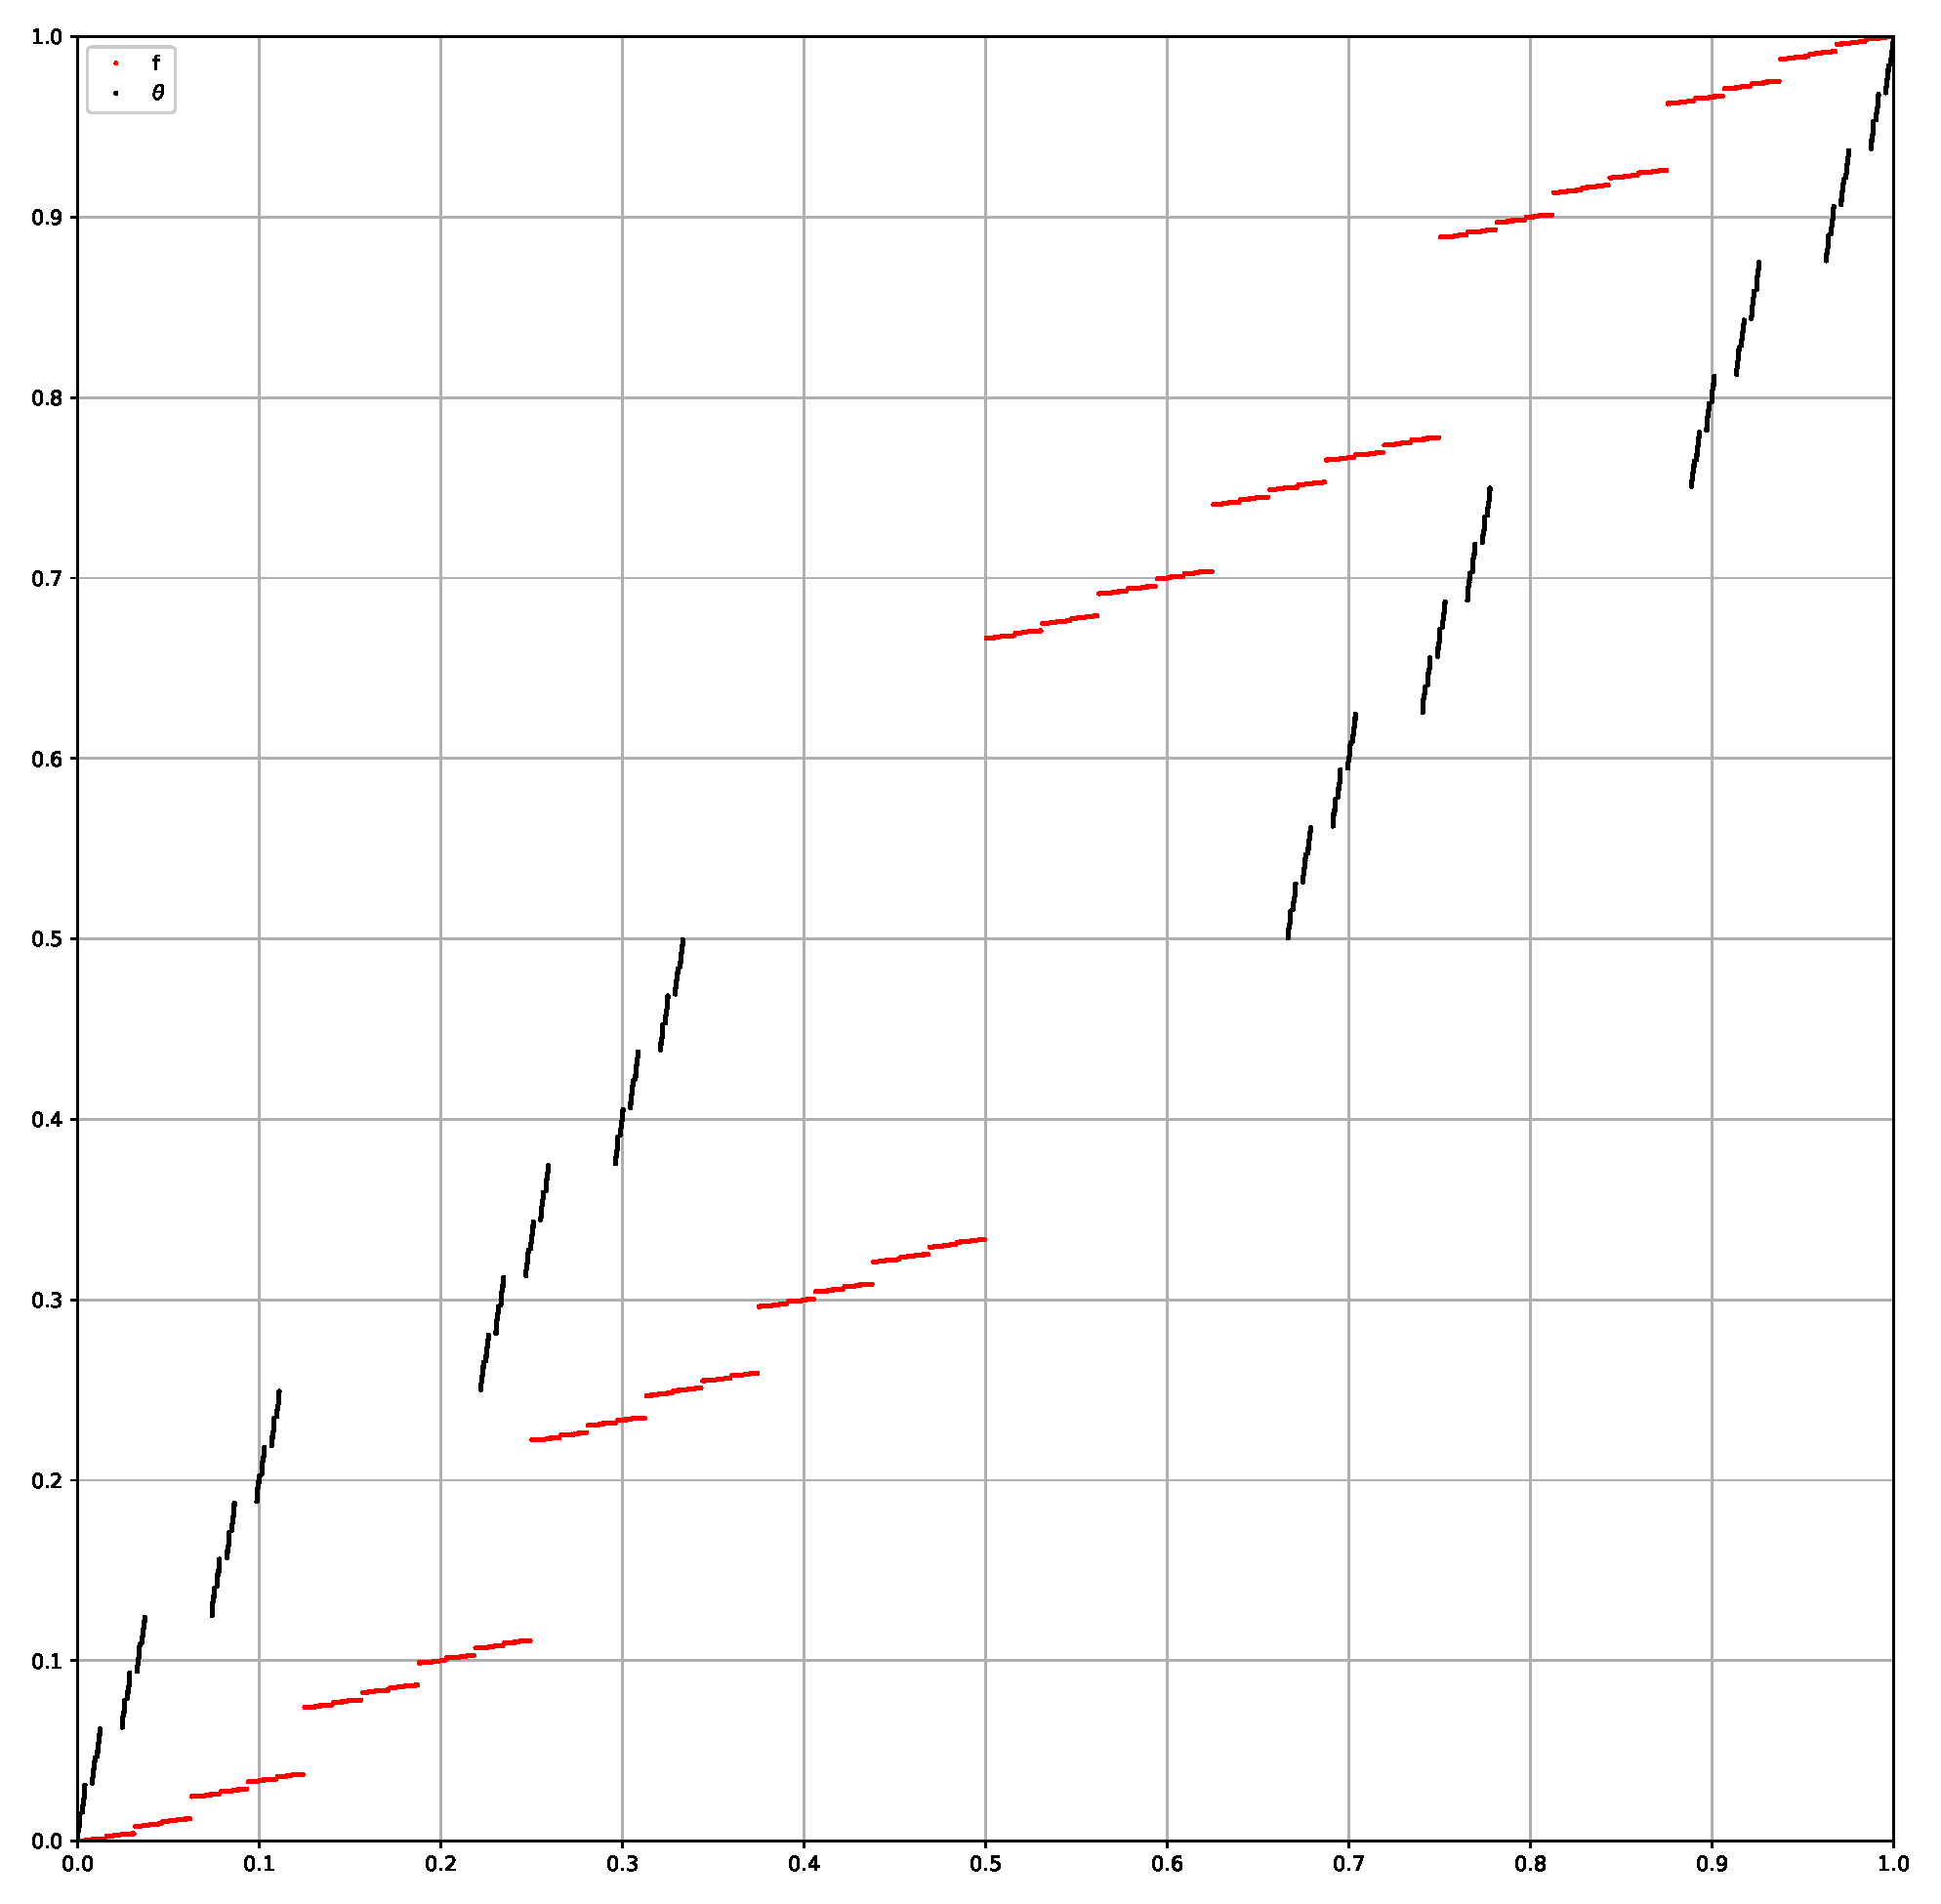
\includegraphics[width=\textwidth]{cantor.eps}
\end{proof}

\newpage
\section{Séance 6}

\begin{ex} Soient $X \neq \emptyset$, $a \in X$ et $\mathcal A = \mathcal P(X)$. Dans l'espace mesuré $(X, \mathcal A, \delta_a)$, montrons que pour $f : X \to \R^+$ mesurable~:
\[\int_X f\dif\delta_a = f(a).\]
\end{ex}

\begin{proof} Supposons d'abord $f$ positive. Soit $g \in \mathcal S^+(X, \mathcal A)$. Pour $(a_i)_{i=1}^k$ les valeurs prises par $g$, par définition on a~:
\[\int g\dif\delta_a = \sum_{i=1}^ka_i\mu(g^{-1}(\{a_i\})) = a_\ell\delta_a(g^{-1}(\{a_\ell\})) = a_\ell = g(a)\]
où $a_\ell = g(a)$. Dès lors, par définition de l'intégrale d'une fonction positive mesurable~:
\[\int f\dif\delta_a = \sup_{\begin{subarray}{l} g \in \mathcal S^+ \\ g \leq f \end{subarray}}\int g\dif\delta_a.\]

On sait que $f(a)$ majore tous les $g(a)$ pour $g \in \mathcal S^+ \st g \leq f$ donc $\int f\dif\delta_a \leq f(a)$. De plus pour $\tilde g = f(a)\chi_{\{a\}}$, on a
$\tilde g \in \mathcal S^+$ et $\tilde g \leq f$, or $\int \tilde g\dif\delta_a = \tilde g(a) = f(a)$. Donc $\int f\dif\delta_a \geq f(a)$. On a alors bien l'égalité.

Dans le cas général où $f$ n'est pas non-négative, soit $f(a) \geq 0$ et donc $f$ est égale à une fonction positive $\delta_a$-ae, soit $f(a) < 0$ et donc $\int f^+\dif\delta_a = 0$,
donc $\int f\dif\delta_a = -\int f^-\dif\delta_a = -f^-(a) = f(a)$.
\end{proof}

\begin{ex} Sur l'espace mesurable $(\R, \B)$, on définit la mesure de Lebesgue $\mathcal L$ et la mesure $\mu$ suivante~:
\[\mu : \B \to \overline \R^+ : B \mapsto \sum_{k \in B \cap \Z}\frac 1{1 + (k+1)^2}.\]

Déterminer si les fonctions suivantes sont intégrables~:
\begin{align*}
	f(x) &=
	\begin{cases}
		\pinfty &\text{ si } x=0 \\
		\ln\abs x & \text{ si } 0 < \abs x < 1 \\
		0 &\text{ sinon}
	\end{cases} \\
	g(x) &=
	\begin{cases}
		\frac 1{x^2-1} &\text{ si } \abs x < 1 \text{ et } x \in \Q \\
		\frac 1{\sqrt {\abs x}} &\text{ si } \abs x < 1 \text{ et } x \in \Q^\C\\
		\frac 1{x^2} & \text{ si }\abs x \geq 1
	\end{cases} \\
	h(x) &\equiv 1
\end{align*}
pour les mesures $\mathcal L$ et $\mu$ comme défini ci-dessus (pour $f$ et $h$).
\end{ex}

\begin{proof}~
\begin{itemize}
	\item Pour la fonction $f$~:
	\begin{itemize}
		\item[$\mathcal L$] Utilisons le théorème de convergence monotone, i.e. construisons une suite croissante $(f_n)_{n \geq 1}$ d'applications mesurables telle que
		$f_n \xrightarrow[n \to \pinfty]{} \tilde f$ (où $\tilde f = \restr f{(0, 1)} = f\chi_{(0, 1)}$). Pour $n \geq 1$, posons~:
		\[f_n : \R \to \R : x \mapsto -\chi_{(\frac 1n, 1)}(x)\ln x.\]

		$f_n$ est majorée par $x \mapsto \chi_{(1/n, 1)}(x)\sup_{y \in (1/n, 1)}-\ln(y) = \ln(n)\chi_{(1/n, 1)}(x)$ qui est intégrable. On en déduit que $f_n$ est intégrable.\footnote{
		Ainsi, toute fonction bornée définie sur un ensemble de mesure finie est intégrable.} Par l'exercice~\ref{ex:7.1}, une fonction bornée Riemann-intégrable est Lebesgue-intégrable et
		les intégrales coïncident. On a donc~:
		\[\int f_n\dif\mathcal L = \int_{\frac 1n}^1-\ln(x)\dif x = 1 - \frac {\ln n+1}n.\]

		En appliquant le théorème de convergence monotone, on trouve~:
		\[\int f\dif\mathcal L = \lim_{n \to \pinfty}\int f_n\dif\mathcal L = \lim_{n \to \pinfty}\left(1 - \frac {1+\ln n}n\right) = 1.\]

		De manière similaire, on trouve que $\int f\chi_{(-1, 0)}\dif\mathcal L = 1$, et on en déduit~:
		\[\int f\dif\mathcal L = \int f\chi_{(-1, 0)}\dif\mathcal L + \int f\chi_{(0, 1)}\dif\mathcal L = 1+1 = 2.\]
		\item[$\mu$:]       $f = \chi_{(-1, 1) \setminus \{0\}}\ln\abs \cdot + (\pinfty)\chi_{\{0\}}$. Donc $f \equiv 0$ sur $\R \setminus (-1, 1)$. Or $(-1, 1) \cap \Z = \{0\}$.
		Donc $f = \pinfty\chi_{\{0\}}$ $\mu$-ae où $x \mapsto \pinfty\chi_{\{0\}}(x) \in \mathcal S^+$. On trouve donc~:
		\[\int f\dif\mu = \int \pinfty\chi_{\{0\}}\dif\mu = \pinfty\mu(\{0\}) = \pinfty \cdot \frac 1{1+1} = \pinfty.\]

		On peut également remarquer que pour $g \in \mathcal S^+ \st g \lneqq f$~:
		\[\int g\dif\mu = \int g\chi_{\{0\}}\dif\mu = g(0)\frac 12.\]
		Donc $\sup\{\int g\dif\mu \st g \in \mathcal S^+, g \lneqq f\}$ n'est pas borné.
	\end{itemize}
	\item Pour la fonction $g$~: $g = \abs x^{-1/2}\chi_{(-1, +1)} + x^{-2}\chi_{(\minfty, 1] \cup [1, \pinfty)}$ $\mathcal L$-ae et ces deux fonction sont Riemann-intégrables. Donc
	$g$ est $\mathcal L$-intégrable et~:
	\[\int g\dif \mathcal L = 2\left(\int_0^1x^{-1/2}\dif x + \int_1^\pinfty x^{-2}\dif x\right) = 2(2+1) = 6.\]
	\item Pour la fonction $h \in \mathcal S^+(\R, \B)$~:
	\begin{itemize}
		\item[$\mathcal L$:] $h$ n'est pas $\mathcal L$-intégrable car $\int h\dif\mathcal L = 1\mathcal L(\R) = \pinfty$.
		\item[$\mu$:]        $h$ est $\mu$-intégrable car~:
		\begin{align*}
			\int h\dif\mu &= \mu(\R) = \sum_{k \in \Z}\frac 1{1+(k+1)^2} = \sum_{k \in \N^*}\frac 1{1+(k-1)^2} + \sum_{k \in \N}\frac 1{1+(k+1)^2} \\
				&= \frac 12 + \sum_{k \in \N^*}\frac 1{1+k^2} + \sum_{k \in \N^*}\frac 1{1+k^2} = \frac 12 + 2\sum_{k \in \N^*}\frac 1{1+k^2} \leq \frac 12 + 2\sum_{k \in \N^*}k^{-2} \\
				&= \frac 12 + 2\zeta(2) = \frac 12 + \frac {\pi^2}3 < \pinfty.
		\end{align*}
	\end{itemize}
\end{itemize}
\end{proof}

\begin{ex} Soient $(X, \mathcal A, \mu)$ un espace mesuré et $(f_k)_{k \geq 1}$ une suite de fonctions mesurables telles que~:
\[f_1 \geq f_2 \geq f_3 \geq \ldots \geq 0.\]

On définit $f \coloneqq  \lim_{k \to \pinfty}f_k$ la limite point par point. Mq si $f_1 \in L^1(X, \mathcal A, \mu)$, alors~:
\[\lim_{k \to \pinfty}\int_Xf_k\dif\mu = \int_Xf\dif\mu.\]

Donner un contre-exemple avec $f_1 \not \in L^1(X, \mathcal A, \mu)$.
\end{ex}

\begin{proof} Pour $n \geq 2 : f_n \leq f_1$ donc $f_n$ est intégrable car majorée par une fonction intégrable. Par la convergence dominée, on a $f$ intégrable
également et $\int f_k\dif\mu \xrightarrow[k \to \pinfty]{} \int f\dif\mu$.

Pour un contre-exemple, prenons la suite constante $f_k : x \mapsto x^{-1}$. $\forall x \in X : f_k(x) \xrightarrow[k \to \pinfty]{} x^{-1}$ qui n'est pas intégrable.

On peut aussi prendre la suite $f_k = \frac 1k\chi_{\R^+}$. Pour tout $k \geq 1 : f_k$ n'est pas intégrable car $\int\abs {f_k}\dif\mathcal L = \frac 1k\mathcal L(\R^+) = \pinfty$.
Or $\forall x \in \R : f_k(x) \xrightarrow[k \to \pinfty]{} 0$. Donc $f_k \xrightarrow[k \to \pinfty]{} \mathbf 0 \in L^1$.
Mais $\int f_k\dif\mathcal L \not \to 0 = \int\mathbf 0\dif\mathcal L$.
\end{proof}

\begin{ex} Supposons $\mu(X) \lneqq \pinfty$. Soit $(f_k)_{k \geq 0}$ une suite de fonctions mesurables positives sur $X$ telles que
$f_k \xrightarrow[k \to \pinfty]{CVU \text{ sur }X} f$. Mq si $\forall k \geq 0 : f_k \in L^1(X, \mathcal A, \mu)$, alors~:
\[f \in L^1(X, \mathcal A, \mu) \qquad \text{ et } \qquad \lim_{k \to \pinfty}\int_Xf_k\dif\mu = \int_Xf\dif\mu.\]
\end{ex}

\begin{proof} À $n > 0$ fixé, on a~:
\[f = \abs f = \abs {f_n + f - f_n} \leq \abs {f_n} + \abs {f - f_n}.\]
Dès lors, par monotonie de l'intégrale~:
\[\int f\dif \mu \leq \int f_n\dif \mu + \int \abs {f-f_n}\dif\mu.\]

La convergence uniforme revient à dire~:
\[\forall \varepsilon > 0 : \exists N > 0 \st \forall n > N : \sup_{x \in X}\abs {f - f_n}(x) < \varepsilon.\]
En particulier, il existe $N > 0 \st \forall n > N : \sup_{x \in X}\abs {f - f_n}(x) < 1$. Dès lors pour $n > N$~:
\[\int f\dif\mu \leq \int f_n\dif \mu + \int \abs {f - f_n}\dif \mu \leq \int f_n \dif\mu + \mu(X) < \pinfty\]
car $f_n \in L^1$ et $\mu(X) < \pinfty$.

On en déduit $f \in L^1(X, \mathcal A, \mu)$. De plus~:
\[\abs {\int f_n\dif\mu - \int f\dif\mu} = \abs {\int (f_n-f)\dif\mu} \leq \int \abs {f_n - f}\dif\mu \leq \mu(X)\sup_{x \in X}\abs {f_n-f}(x) \xrightarrow[n \to \pinfty]{} 0,\]
i.e. $\int f_n\dif\mu \xrightarrow[n \to \pinfty]{} \int f\dif\mu$.
\end{proof}

\begin{ex} On définit pour $k \geq 0$~:
\[\alpha_k \coloneqq \int_0^k\left(1 - \frac xk\right)^k\exp(x/2)\dif x \qquad \text{ et } \qquad \beta_k \coloneqq \int_0^k\left(1 + \frac xk\right)^k\exp(-2x)\dif x.\]
Calculer $\alpha \coloneqq \lim_{k \to \pinfty}\alpha_k$ et $\beta \coloneqq \lim_{k \to \pinfty} \beta_k$.
\end{ex}

\begin{proof} On pose $f_k(x) \coloneqq \left(1-\frac xk\right)^ke^{x/2}\chi_{[0, k]}(x)$ et $g_k(x) = \left(1+\frac xk\right)^ke^{-2x}\chi_{[0, k]}(x)$.
Puisque $f_k(x) \nearrow e^{-x/2}\chi_{\R^+}(x)$ et $g_k(x) \nearrow e^{-x}\chi_{\R^+}(x)$ (deux limites $\in L^1$), par la convergence dominée, on a~:
\[\lim_{k \to \pinfty} \alpha_k = \lim_{k \to \pinfty}\int f_k\dif\mu = \int\lim_{k \to \pinfty}f_k\dif\mu = [2e^{x/2}]_{\minfty}^0 = 2,\]
et~:
\[\lim_{k \to \pinfty}\beta_k = \lim_{k \to \pinfty}\int g_k\dif\mu = \int\lim_{k \to \pinfty}g_k\dif\mu = [-e^{-x}]_0^\pinfty = 1.\]
\end{proof}

\begin{ex}\label{ex:6.6} Soit $f \in L^1(X, \mathcal A, \mu)$. Mq~:
\[\forall \varepsilon > 0 : \exists \delta > 0 \st \forall A \in \mathcal A : \mu(A) < \delta \Rightarrow \int_A\abs f\dif\mu < \varepsilon.\]
\end{ex}

\begin{proof} Par l'absurde, supposons qu'il existe $\varepsilon > 0 \st$~:
\[\forall n > 0 : \exists A_n \in \mathcal A \st \mu(A_n) < \frac 1n \text{ et } \int_{A_n}f\dif \mu \geq \varepsilon.\]

Posons $f_n \coloneqq f\chi_{A_n}$. $\forall n > 0 : \abs {f_n} \leq \abs f$ et $\abs {\lim_{n \to \pinfty}f_n} \leq \abs f$ et ces applications sont mesurables. Donc par
la convergence dominée, on a~:
\[\lim_{n \to \pinfty}\int f_n\dif\mu = \int\lim_{n \to \pinfty}f_n\dif \mu.\]

Mq $\lim_{n \to \pinfty}f_n = 0$ $\mu$-ae. Soit $N \coloneqq \{x \in X \st \lim_{n \to \pinfty}f_n(x) \neq 0\}$. Soit $x \in N$. On sait que~:
\[\exists K > 0 \st \forall k \geq K : x \in A_k \qquad\text{ i.e. }\qquad x \in \bigcup_{K > 0}\bigcap_{k \geq K}A_k = \liminf_{k \to \pinfty}A_k.\]
Donc $N \subseteq \liminf_{k \to \pinfty}A_k$, et par monotonie de la mesure (et par l'exercice~\ref{ex:2.9})~:
\[\mu(N) \leq \mu\left(\liminf_{k \to \pinfty}A_k\right) \leq \liminf_{k \to \pinfty}\mu(A_k) = \lim_{k \to \pinfty}\mu(A_k) = \lim_{k \to \pinfty} \frac 1k = 0.\]
Donc $f_n \xrightarrow[n \to \pinfty]{\mu\text{-ae}} \mathbf 0$. Finalement, on déduit~:
\[\varepsilon \leq \lim_{n \to \pinfty}\int f_n\dif \mu = \int\lim_{n \to \pinfty}f_n\dif \mu = \int\mathbf 0\dif\mu = 0,\]
ce qui est une contradiction.
\end{proof}

\newpage
\section{Séance 7}
\begin{ex}\label{ex:7.1}
Soit $f : [a, b] \to \R$ bornée. Mq~:
\begin{enumerate}
	\item si $f$ est Riemann-intégrable, alors $f$ est Lebesgue-intégrable et~:
	\[\int_a^bf(x)\dif x = \int_{[a, b]}f\dif\mathcal L.\]
	\item les fonctions $h$ et $H$ définies ci-dessous sont bien définies et $h \leq f \leq H$ sur $[a, b]$~:
	\begin{align*}
		h(x) &= \lim_{\delta \to 0}\inf_{\abs {y-x}<\delta}f(y), \\
		H(x) &= \lim_{\delta \to 0}\sup_{\abs {y-x}<\delta}f(y).
	\end{align*}
	\item $f$ est continue en $x$ ssi $H(x) = h(x)$.
	\item $H$ et $h$ sont Lebesgue-mesurables et~:
	\[\int_{[a, b]}H\dif\mathcal L = \inf_PU(f; P) \qquad \text{ et } \qquad \int_{[a, b]}h\dif\mathcal L = \sup_PL(f; P).\]
	\item En déduire que $f$ est Riemann-intégrable ssi l'ensemble des discontinuités de $f$ est négligeable.
\end{enumerate}
\end{ex}

\begin{proof}~
\begin{enumerate}
	\item \underline {\textbf {Notations}~:}
	Pour $P = (x_i)_{i=0}^{N_P}$ une partition de $[a, b]$, on pose pour $i \in \intint 0{N_P-1} : P(i] \coloneqq (x_i, x_{i+1}]$. On pose également les fonctions~:
	\begin{align*}
		f_P &\coloneqq \sum_{j=0}^{N_P - 1}m_j\chi_{P(j]} + f(a)\chi_{\{a\}} \\
		f^P &\coloneqq \sum_{j=0}^{N_P - 1}M_j\chi_{P(j]} + f(a)\chi_{\{a\}}
	\end{align*}

	Pour $P$ une partition de $[a, b]$ et $y \in (a, b) \st \forall i \in \intint 0{N_P}$, on pose $P \oplus y \coloneqq (x'_j)_{j=0}^{N_P+1}$ où
	$\exists j \in \intint 1{N_P} \st x'_j = y$ et $(x'_1, \ldots, x'_{j-1}, x'_{j+1}, \ldots, x'_{N_P+1}) = P$. Pour deux partitions
	$P_1 = (x_{1,j})_{j=0}^{N_{P_1}}$ et $P_2 = (x_{2,j})_{j=0}^{N_{P_2}}$, on pose également $P_1 \oplus P_2$ la plus petite partition $(x_j)_{j=0}^{N_P}$ où~:
	\[\forall j \in \intint 0{N_{P_1}} : \forall \ell \in \intint 0{N_{P_2}} : \exists i, k \in \intint 0{N_P}	\st x_{1,j} = x_i \text{ et } x_{2,\ell} = x_k.\]

	\underline {\textbf {Résolution}~:}

	Observons que pour une partition $P$ et $y \in (a, b)$, on a~:
	\begin{itemize}
		\item $f^{P \oplus y} \leq f^P$~;
		\item $f_{P \oplus y} \geq f_P$.
	\end{itemize}

	En effet, cela découle directement du fait que pour $P \oplus y = (x'_j)_{j=0}^{N_P+1}$ et pour $j \st y = x'_j$~:
	\[\inf_{t \in (x_j, x_{j+1}]}f(t) \geq \inf_{t \in (x_{j-1}, x_{j+1}]}f(t) \quad\text{ et }\quad \inf_{t \in (x_{j-1}, x_j]}f(t) \geq \inf_{t \in (x_{j-1}, x_{j+1}]}f(t).\]
	On déduit similairement pour le $\sup$~:
	\[\sup_{t \in (x_j, x_{j+1}]}f(t) \leq \sup_{t \in (x_{j-1}, x_{j+1}]}f(t) \quad\text{ et }\quad \sup_{t \in (x_{j-1}, x_j]}f(t) \leq \sup_{t \in (x_{j-1}, x_{j+1}]}f(t).\]

	Ainsi, on remarque que pour deux partitions $P_1$ et $P_2$, on a les inégalités suivantes par le même raisonnement~:
	\begin{itemize}
		\item $f^{P_1 \oplus P_2} \leq f^{P_1}$~;
		\item $f_{P_1 \oplus P_2} \geq f_{P_1}$.
	\end{itemize}

	Par définition de $\inf/\sup$, il existe une suite de partitions $(P'_n)_{n \geq 0} \st U(f; P'_n) \xrightarrow[n \to \pinfty]{} \inf_PU(f; P)$ et
	une suite de partitions $(\tilde P_n)_{n \geq 0} \st L(f; \tilde P_n) \xrightarrow[n \to \pinfty]{} \sup_PL(f; P)$. De plus les suites $(U(f; P'_n))_{n \geq 0}$
	et $(L(f; \tilde P_n))_{n \geq 0}$ sont respectivement décroissante et croissante. Par la remarque ci-dessus, on remarque que si on pose $P_n \coloneqq P'_n \oplus \tilde P_n$,
	on obtient une suite de partitions $(P_n)_n$ telle que~:
	\[\lim_{n \to \pinfty}U(f; P_n) = \inf_PU(f; P) = \sup_PL(f; P) = \lim_{n \to \pinfty} L(f; P_n).\]
	En particulier~: $U(f; P_n) - L(f; P_n) \xrightarrow[n \to \pinfty]{} 0$.

	Remarquons ensuite que les $f_{P_n}$ sont des applications mesurables puisque des des combinaisons linéaires de fonctions caractéristiques sur des boréliens (en effet
	les intervalles ouverts à gauches sont des boréliens et le singleton $\{a\}$ en est un également). De plus~:
	\[\int_{[a, b]} f_{P_n}\dif\mathcal L = L(f; P_n) \quad\text{ et }\quad \int_{[a, b]} f^{P_n}\dif\mathcal L = U(f; P_n).\]

	Puisque $U(f; P_n) - L(f; P_n) \xrightarrow[n \to \pinfty]{} 0$, on a $\int_{[a, b]}(f^{P_n}-f_{P_n})\dif \mathcal L \xrightarrow[n \to \pinfty]{} 0$.
	Du coup $\lim_{n \to \pinfty}(f^{P_n} - f_{P_n}) = 0$ $\mathcal L$-ae, i.e. $f_{P_n} \xrightarrow[n \to \pinfty]{\mathcal L\text{-ae}} f$

	Dès lors, par le théorème de la convergence monotone, on a que $f$ est mesurable et que~:
	\[\int_{[a, b]} f\dif\mathcal L = \int_{[a, b]} \lim_{n \to \pinfty}f_{P_n}\dif\mathcal L = \lim_{n \to \pinfty}\int_{[a, b]}f_{P_n}\dif\mathcal L = \lim_{n \to \pinfty}L(f; P_n)
	= \sup_PL(f; P) = \int_a^bf(x)\dif x.\]

	\item Puisque $f$ est bornée, pour tout $x \in [a, b], \delta \gneqq 0$, on a bien~:
	\[\abs {\inf_{y \in B_\delta(x) \cap [a, b]}f(y)} \lneqq \pinfty \quad\text{ et }\quad \abs {\sup_{y \in B_\delta(x) \cap [a, b]}f(y)} \lneqq \pinfty.\]

	De plus, pour tout $x \in [a, b], \delta \gneqq 0$~:
	\[\inf_{y \in B_\delta(x) \cap [a, b]} f(y) \leq f(x) \leq \sup_{y \in B_\delta(x) \cap [a, b]}f(y).\]

	\item \underline {$\Leftarrow$~:} $H(x) = h(x)$ est équivalent à~:
	\[\forall \varepsilon > 0 : \exists \delta_\varepsilon > 0 \st \forall \gamma > 0 : \gamma \leq \delta_\varepsilon \Rightarrow
	\sup_{y \in B_\gamma(x)}f(y) - \inf_{y \in B_\gamma(x)}f(y) \leq \varepsilon.\]

	En particulier, à $\varepsilon > 0$ fixé, pour $y \in [a, b]$, si $\abs {x-y} \leq \delta_\varepsilon$, alors~:
	\[\abs {f(x)-f(y)} \leq \sup_{z \in B_{\delta_\varepsilon}(x)}f(z) - \inf_{z \in B_{\delta_\varepsilon}}f(z) \leq \varepsilon.\]
	On a donc bien la continuité de $f$ en $x$.

	\underline {$\Rightarrow$~:} à $\varepsilon > 0$ fixé, il existe $\delta > 0 \st \abs {x-y} < \delta \Rightarrow \abs {f(x)-f(y)} < \varepsilon$. Donc~:
	\begin{align*}
		\sup_{y \in B_\delta(x)}f(y) - \inf_{y \in B_\delta(x)}f(y) &= \left(\sup_{y \in B_\delta(x)}f(y) - f(x)\right) - \left(\inf_{y \in B_\delta(x)}f(y) - f(x)\right) \\
		&\leq \abs {\sup_{y \in B_\delta(x)}f(y)-f(x)} + \abs {f(x)-\inf_{y \in B_\delta(x)}f(y)} \leq 2\varepsilon.
	\end{align*}

	Or cette inégalité est vraie pour tout $\varepsilon > 0$. On en déduit que $H(x)-h(x) = 0$.

	\item Reconsidérant maintenant la suite $(P_n)_{n \geq 0} \st U(f; P_n) \xrightarrow[n \to \pinfty]{} \inf_PU(f; P)$ et $L(f; P_n) \xrightarrow[n \to \pinfty]{} \sup_PL(f; P)$
	et supposons-la croissante (ce qui n'est pas abusif~: il suffit de poser la suite de partitions $\hat P_0 \coloneqq P_0$ et $\hat P_n \coloneqq \hat P_{n-1} \oplus P_n$
	qui est croissante au sens de l'inclusion et qui satisfait les limites puisque $f^{\hat P_n} \leq f^{P_n}$ et $f_{\hat P_n} \geq f_{P_n}$).
	Pour toute partition $P$ et pour tout $x \in [a, b] \setminus P$, on note $j_{P,x} \in \intint 0{N_P-1} \st x \in P(j_{P,x}]$. Fixons alors $x \in [a, b] \setminus
	\bigcup_{n \geq 0}P_n$ (i.e. $\forall n \geq 0 : x \not \in P_n$).

	Séparons deux cas~:
	\begin{itemize}
		\item[{si $\mathcal L(P_n(j_{P_n,x}]) \xrightarrow[n \to \pinfty]{} 0$}~:] $\forall \delta > 0 : \exists N > 0 \st P_N(j_{P_N,x}] \subset B_\delta(x)$.
		Posons une suite $(\delta_n)_{n \geq 0}$ décroissante vers 0 et posons $H_n(x) \coloneqq \sup_{y \in B_{\delta_n}(x)}f(y)$.

		On remarque que $\forall n \geq 0 : \exists K > 0 \st \forall k \geq K : H_n(x) \geq f^{P_k}(x) \geq H(x)$. Or $H_n(x) \xrightarrow[n \to \pinfty]{} H(x)$, et donc
		$f^{P_n}(x) \xrightarrow[n \to \pinfty]{} H(x)$.

		\item[sinon~:] $\forall (\alpha, \beta] \subset \bigcap_{n \geq 0}P_n(j_{P_n, x}] : \exists K > 0 \st \forall k \geq K :$
		\[\sup_{y \in (\alpha, \beta]}f(y) = \sup_{y \in P_k(j_{P_k, x}]}f(y).\]

		En effet, s'il existe $(\alpha, \beta]$ qui ne satisfait pas la propriété, alors les $P_n$ pourraient être raffinés par la suite $(P'_n)_{n \geq 0}$ définie par
		$P'_n \coloneqq P_n \oplus \alpha \oplus \beta$. Dans ce cas~: $f^{P_n} \gneqq f^{P'_n}$ sur $[\alpha, \beta]$, ce qui contredit~:
		\[U(f; P_n) \xrightarrow[n \to \pinfty]{} \inf_PU(f; P).\]

		On déduit donc~:
		\[\lim_{\delta \to 0}\sup_{y \in B_\delta(x)}f(y) = \sup_{y \in \bigcap_{n \geq 0}P_n(j_{P_n,x}]}f(y),\]
		i.e.~:
		\[H(x) = \lim_{\delta \to 0}\sup_{y \in B_\delta(x)}f(y) = \sup_{y \in \bigcap_{n \geq 0}P_n(j_{P_n,x}]}f(y) = \lim_{n \to \pinfty}f^{P_n}(x).\]
	\end{itemize}
	On déduit de ces deux cas $f^{P_n} \xrightarrow[n \to \pinfty]{\mathcal L\text{-ae}} H$ et donc $H$ est mesurable puisque limite de fonctions mesurables. De plus, on sait
	que pour toute partition $P$~: $f^P$ est $\mathcal L$-intégrable sur $[a, b]$ car $f$ est majorée par $M \gneqq 0$ et donc~:
	$\int_{[a, b]} \abs {f^P}\dif\mathcal L \leq M\mathcal L([a, b]) \lneqq \pinfty$. Dès lors,
	par le théorème de la convergence dominée~:
	\[\int H\dif\mathcal L = \lim_{n \to \pinfty}\int f^{P_n}\dif\mathcal L = \inf_PU(f; P).\]
	On déduit similairement le cas $\int h\dif\mathcal L = \sup_PL(f; P)$.

	\item $f$ est Riemann-intégrable $\iff \int H\dif\mathcal L = \int h\dif\mathcal L \iff \int (H-h)\dif\mathcal L = 0 \iff H = h$ $\mathcal L$-ae
	et donc $\iff \mathcal L(\{x \in [a, b] \st H(x) \neq h(x)\}) = 0$, i.e. $f$ est continue $\mathcal L$-ae.
\end{enumerate}
\end{proof}

\begin{ex}~
\begin{enumerate}
	\item Mq si $f : [a, \pinfty) \to \R$ est Riemann-intégrable et bornée sur $[a, b]$ pour tous $b > a$, alors~:
	\[\int_{[a, \pinfty)}f\dif\mathcal L = \int_a^\pinfty f(x)\dif x.\]
	\item Mq si $f : [a, b] \to \R$ est Riemann-intégrable et bornée sur $[c, b]$ pour tous $c \in (a, b)$, alors~:
	\[\int_{[a, b]}f\dif\mathcal L = \int_a^bf(x)\dif x.\]
\end{enumerate}
\end{ex}

\begin{proof}~
\begin{enumerate}
	\item Posons la suite croissante de fonctions $f_n \coloneqq f\chi_{[a, a+n]}$. Puisque les $f_n$ sont bornées et Riemann-intégrables (par hypothèse), par l'exercice précédent,
	on sait que les $f_n$ sont mesurables et que $\int_{[a, a+n]}f\dif\mathcal L = \int_a^{a+n}f(x)\dif x$. Puisque $f_n \xrightarrow[n \to \pinfty]{} f$, on
	a que $f$ est mesurable. De plus, par le théorème de la convergence monotone~:
	\[\int f\dif\mathcal L = \lim_{n \to \pinfty}\int f_n\dif\mathcal L = \lim_{n \to \pinfty}\int_a^{a+n}f(x)\dif x = \int_a^\pinfty f(x)\dif x.\]

	\item De manière similaire, on pose la suite croissante de fonctions $f_n \coloneqq f\chi_{[a+\frac 1n, b]}$ qui converge vers $f$ sur $(a, b]$ (donc $\mathcal L$-ae).
	Puisque les $f_n$ sont mesurables, on déduit à nouveau que $f$ est mesurable également et par la convergence monotone~:
	\[\int f\dif\mathcal L = \lim_{n \to \pinfty}\int f_n\dif\mathcal L = \lim_{n \to \pinfty}\int_{a+\frac 1n}^bf(x)\dif x = \int_a^bf(x)\dif x.\]
\end{enumerate}
\end{proof}

\begin{ex} $\Q$ est dénombrable donc $\Q \cap [0, 1]$ l'est aussi. Donc $\Q \cap [0, 1] = \{q_k\}_{k \geq 0}$. Pour $k \geq 0$, on définit~:
\[f_k : [0, 1] \to \R : x \mapsto \begin{cases}1 &\text{ si } x \in \{q_\ell\}_{\ell=0}^k \\0 &\text{ sinon}.\end{cases}\]

\begin{enumerate}
	\item Mq $\forall k \geq 0 : f_k$ est Riemann-intégrable et déterminer~:
	\[\int_0^1f_k(x)\dif x.\]
	\item Mq $f_k \xrightarrow[k \to \pinfty]{CVS \text{ sur } [0, 1]} f$. Que peut-on en déduire~?
	\item Mq $f$ est Lebesgue-intégrable et vérifier les hypothèses du théorème de la convergence dominée.
\end{enumerate}
\end{ex}

\begin{proof}~
\begin{enumerate}
	\item À $k$ fixé, $f_k$ est bornée sur son compact de définition et est continue sur $[0, 1] \setminus \{q_\ell\}_{\ell=0}^k$, donc $f_k$ est Riemann-intégrable. De plus~:
	\[\int_0^1f_k(x)\dif x = \sum_{\ell=1}^k\int_{q_{\ell-1}}^{q_\ell}f_k(x)\dif x = \sum_{\ell=1}^k0 = 0.\]

	De manière plus élégante, remarquons que $f_k$ est la fonction caractéristique d'un ensemble de mesure nulle, donc $f_k$ est mesurable et de plus~:
	\[\int f_k\dif\mathcal L = \mathcal L(\{q_\ell\}_{\ell=0}^k) = 0,\]
	donc $f_k$ est Lebesgue-intégrable. De plus $f_k$ est bornée sur son compact de définition (qui est forcément de mesure finie), donc $f_k$ doit être Riemann-intégrable.

	\item Soit $x \in [0, 1]$. Si $x \in \Q^\C$, alors $\forall k \geq 0 : f_k(x) = 0$. Si $x \in \Q$, alors $\exists K \geq 0 \st x = q_K$, ce qui implique
	$\forall k \geq K : f_k(x) = 1$. Donc $f_k \xrightarrow[k \to \pinfty]{} \chi_{\Q \cap [0, 1]}$. Notons que $f_k$ converge simplement mais pas uniformément. En effet~:
	\[\forall k \geq 0 : \sup_{x \in [0, 1]}\abs {f_k(x)-\chi_\Q(x)} = 1.\]

	Puisque $\chi_{\Q \cap [0, 1]}$ n'est pas Riemann-intégrable, on a l'existence d'une fonction $\mathcal L$-intégrable mais pas R-intégrable.

	\item Voir la remarque ci-dessus pour l'intégrabilité au sens de Lebesgue. Les $f_k$ sont bien mesurables et $f = \chi_{\Q \cap [0, 1]} \leq \chi_{[0, 1]}$ qui est intégrable.
	Donc par la convergence dominée, on a bien $\int f\dif\mathcal L = 0$.
\end{enumerate}
\end{proof}

\newpage
\section{Séance 8}
\begin{ex} Soit $(X, \mathcal A, \mu)$ un espace mesuré.
\begin{enumerate}
	\item Si $\mu(X) \lneqq \pinfty$, mq si $p$ et $q$ sont des réels tels que $1 \leq q \lneqq p \lneqq \pinfty$, alors~:
	\[L^\infty(X, \mathcal A, \mu) \subseteq L^p(X, \mathcal A, \mu) \subset L^q(X, \mathcal A, \mu) \subset L^1(X, \mathcal A, \mu).\]
	\item Considérons la fonction suivante~:
	\[u : \R \to \R : x \mapsto \begin{cases}x^{\frac {-1}q} &\text{ si } x \geq 1 \\0 &\text{ sinon}.\end{cases}\]
	Mq $u \in L^p(\R) \setminus L^q(\R)$.
	\item Considérons la fonction suivante~:
	\[v : \R \to \R : x \mapsto \begin{cases}x^{\frac {-1}p} &\text{ si } x \in (0, 1] \\0 &\text{ sinon}.\end{cases}\]
	Mq $u \in L^q(\R) \setminus L^p(\R)$.
	\item A-t-on $L^q(\R) \subseteq L^\infty(\R)$ et $L^\infty(\R) \subseteq L^q(R)$~?
\end{enumerate}
\end{ex}

\begin{proof}~
\begin{enumerate}
	\item~
	\begin{itemize}
		\item[$L^\infty \subseteq L^p$~:] Soit $f \in L^\infty$. $\mu$ étant une mesure finie, les ensembles $\mu$-négligeables et localement-$\mu$-négligeables coïncidente.
		Il existe donc $C \geq 0 \st \mu(\{x \in X \st \abs {f(x)} > C\}) = 0$. Notons cet ensemble $N$. On a alors~:
		\[\int \abs f^p\dif\mu = \int_N\abs f^p\dif\mu + \int_{N^\C}f^p\dif\mu \leq C^p\mu(N^\C) = C^p\mu(X) < \pinfty.\]

		\item[$L^p \subseteq L^q$~:] Soit $f \in L^p$. On remarque que $\abs f^q \in L^{\frac pq}$ avec $\frac pq > 1$. De plus, puisque $\mu(X) < \pinfty$, les fonctions constantes
		sont intégrables  (car dans $L^\infty$). En particulier $\mathbf 1 : x \mapsto 1$ est dans $L^{\frac p{p-q}}$. Par Hölder~:
		\[\norm f_{L^q}^q = \norm {f^q}_{L^1} = \norm {\abs f^q\abs {\mathbf 1}^{\frac p{q-p}}}_{L^1} = \int\abs f^q\dif\mu = \int\abs f^q\abs {\mathbf 1}\dif\mu
			\leq \norm {\abs f^q}_{L^{\frac pq}}\underbrace {\norm {\mathbf 1}_{L^{\frac p{p-q}}}}_{= \mu(X) < \pinfty}.\]
		Or~:
		\[\left[\int \left(\abs f^q\right)^{\frac pq}\dif\mu\right]^{\frac qp} = \left[\int \abs f^p\dif\mu\right]^{\frac qp} = \left[\left(\int \abs f^p\dif\mu\right)^{\frac 1p}\right]^q
		= \norm f_{L^p}^q < \pinfty.\]

		Donc $f \in L^q$.

		\item[$L^q \subseteq L^1$~:] Soit $f \in L^q$. $f = f\chi_A + f\chi_{A^\C}$ où $A = \{x \in X \st \abs {f(x)} \geq 1\}$. Donc~:
		\[\int \abs f\dif\mu = \int_A\abs f\dif\mu + \int_{A^\C}\abs f\dif\mu \leq \int_A\abs f^q\dif\mu + \int_{A^\C}1\dif\mu \leq \norm f_{L^q}^q + \mu(A^\C) < \pinfty.\]
	\end{itemize}

	\item $u \in L^p$ pour $p > q$ car~:
	\[\int u^p\dif\mathcal L = \lim_{t \to \pinfty}\int_1^tx^{-\frac pq}\dif x = \frac {-q}{p-q}\lim_{t \to \pinfty}\left(t^{-\frac {p-q}q} - 1\right) = \frac q{p-q}\]
	car $\frac {p-q}q > 0$ et donc $t^{-\frac {p-q}q} \xrightarrow[t \to \pinfty]{} 0$.

	De plus $u \not \in L^q$ car~:
	\[\int u^q\dif\mathcal L = \lim_{t \to \pinfty}\int_1^tx^{-1}\dif x = \lim_{t \to \pinfty}\ln(t) = \pinfty.\]

	\item $v \in L^q$ pour $q < p$ car~:
	\[\int v^q\dif\mathcal L = \lim_{\varepsilon \to 0}\int_\varepsilon^1x^{-\frac qp}\dif x = \frac q{p-q}\lim_{\varepsilon \to 0}\left(1 - \varepsilon^{\frac {p-q}q}\right)
	= \frac q{p-q}\]
	car $\frac {p-q}q > 0$.

	De plus $v \not \in L^p$ car~:
	\[\int v^p\dif\mathcal L = \lim_{\varepsilon \to 0}\int_\varepsilon^1x^{-1}\dif x = 1 - \lim_{\varepsilon \to 0}\ln\varepsilon = \pinfty.\]

	\item $L^\infty(\R) \not \subseteq L^q(\R)$ car $\norm {\mathbf 1}_{L^\infty} = 1 \lneqq \pinfty$ mais $\forall q \in [1, \pinfty)$~:
	$\norm {\mathbf 1}_{L^q} = \mathcal L(\R) = \pinfty$. L'autre inclusion ne tient pas non plus~: $f : x \mapsto x^{-\frac 1{2q}}\chi_{(0, 1)}$ est dans $L^q$ car~:
	\[\norm {f}_{L^q}^q = \int \abs {x^{-\frac 1{2q}}}^q\chi_{(0, 1)}\dif \mathcal L(x) = \int_0^1x^{-\frac 12}\dif\mathcal L(x) = 2 \lneqq \pinfty.\]
	Or $\norm f_{L^\infty} = \pinfty$ car~:
	\[\forall M > 0 : \mathcal L(\{x \in (0, 1) \st f(x) \geq M\}) = \mathcal L(\{x \in (0, 1) \st M^{-1} \geq \sqrt x\}) = \mathcal L((0, M^{-2})) = M^{-2} > 0.\]
\end{enumerate}
\end{proof}

\begin{ex}[Inégalité de Chebycshev] Soient $(X, \mathcal A, \mu)$ un espace mesuré et $f : X \to [0, \pinfty)$ une application mesurable. Mq
\[\forall \alpha > 0 : \mu\left(\left\{x \in X \st f(x) \geq \alpha\right\}\right) \leq \frac 1\alpha\int f\dif\mu.\]

De plus, si $\Phi : \R^+ \to \R^+$ est une application mesurable croissante, alors~:
\[\forall \alpha > 0 : \mu\left(\left\{x \in X \st f(x) \geq \alpha\right\}\right) \leq \frac 1{\Phi(\alpha)}\int \Phi(f(x))\dif\mu(x).\]
\end{ex}

\begin{proof} à $\alpha > 0$ fixé, notons $A_\alpha(f) \coloneqq \{x \in X \st f(x) \geq \alpha\}$. L'inégalité découle simplement du fait que~:
\[\int_Xf\dif\mu \geq \int_{A_\alpha(f)}f\dif\mu \geq \int_{A_\alpha(f)}\alpha\dif\mu = \alpha\mu(A_\alpha(f)).\]

Pour le second point, il suffit de remarquer que $A_\alpha(f) \subset A_{\Phi(\alpha)}(\Phi \circ f)$ puisque $\Phi$ est croissante. Donc en appliquant le premier point~:
\[\mu(A_\alpha(f)) \leq \mu(A_{\Phi(\alpha)}(\Phi \circ f)) \leq \frac 1{\Phi(\alpha)}\int\Phi\circ f\dif\mu.\]
\end{proof}

\begin{ex} Soient $(X, \mathcal A, \mu)$ un espace mesuré et $f : X \to \R$ une application mesurable.
\begin{enumerate}
	\item Mq~:
	\[\liminf_{p \to \pinfty}\norm f_{L^p} \geq \norm f_{L^\infty},\]
	et donner un exemple où l'inégalité est infinie à gauche et finie à droite.
	\item Supposions qu'il existe $q \in [1, \pinfty) \st f \in L^q(X)$.
	\begin{enumerate}
		\item Mq $f$ est finie $\mu$-ae.
		\item Supposons que $0 \lneqq \norm f_{L^\infty} \lneqq \pinfty$. Mq si $p \in (q, \pinfty)$, alors~:
		\[\norm f_{L^p} \leq \norm f_{L^\infty}^{1-\frac qp} \cdot \norm f_{L^q}^{\frac qp},\]
		et en déduire que~:
		\[\limsup_{p \to \pinfty} \norm f_{L^p} \leq \norm f_{L^\infty}.\]
		\item Conclure.
	\end{enumerate}
\end{enumerate}
\end{ex}

\begin{proof}~
\begin{enumerate}
	\item Séparons les cas $(i)~\norm f_{L^\infty} = 0~; \, (ii)~\norm f_{L^\infty} \lneqq \pinfty$ et $(iii)~\norm f_{L^\infty} = \pinfty$.
	\begin{itemize}
		\item Dans le premier cas, puisque $\forall p \geq 1 : \norm f_{L^p} \geq 0$, l'inégalité est triviale.
		\item Dans le second cas, l'inégalité est\ldots~moins triviale.

		Séparons à nouveau deux cas ici~: soit $\forall p \geq 1 : f \not \in L^p(X)$ soit $\exists p \geq 1 \st f \in L^p$. Dans le premier cas, on a donc
		$\forall p \geq 1 : \norm f_{L^p} = \pinfty \geq \norm f_{L^\infty}$, donc ok. Supposons donc alors qu'il existe $\widetilde p \geq 1 \st f \in L^{\widetilde p}$.
		On pose alors une suite $(\varepsilon_n)_{n \geq 0}$ telle que $\forall n \geq 0 : 0 < \varepsilon_n < \norm f_{L^\infty}$ et $\varepsilon_n \searrow 0$.
		Pour tout $n \geq 0$, on pose~:
		\[\Omega_{\varepsilon_n} \coloneqq \{x \in X \st \abs {f(x)} \geq \norm f_{L^\infty}-\varepsilon_n\} = f^{-1}\left((\norm f_{L^\infty}-\varepsilon_n, \pinfty)\right).\]

		Puisque $(\varepsilon_n)_{n \geq 0}$ décroit, la suite $(\Omega_{\varepsilon_n})_{n \geq 0}$ décroit également. De plus, par définition du supremum essentiel ($\norm f_{L^\infty}$),
		on déduit $\mu(\Omega_{\varepsilon_n}) \gneqq 0$. Maintenant observons que, à $p \geq 1$ et $n \geq 0$ fixés~:
		\[\norm f_{L^p} = \left(\int_X\abs f^p\dif\mu\right)^{\frac 1p} \geq \left(\int_{\Omega_{\varepsilon_n}}\abs f^p\dif\mu\right)^{\frac 1p}
		\geq \left(\int_{\Omega_{\varepsilon_n}}\left(\norm f_{L^\infty}-\varepsilon_n\right)^p\dif\mu\right)^\frac 1p
		= \left(\norm f_{L^\infty}-\varepsilon_n\right)\mu(\Omega_{\varepsilon_n})^{\frac 1p}.\]

		Montrons alors que $\mu(\Omega_{\varepsilon_n}) \lneqq \pinfty$. Puisque $\norm f_{L^{\widetilde p}} \lneqq \pinfty$, on sait~:
		\[\pinfty \gneqq \norm f_{L^{\widetilde p}} \geq \underbrace {\left(\norm f_{L^\infty}-\varepsilon_n\right)}_{\lneqq \pinfty}\mu\left(\Omega_{\varepsilon_n}\right)^{\frac 1{\widetilde p}}.\]
		On a donc obligatoirement $\mu(\Omega_{\varepsilon_n}) \lneqq \pinfty$.

		Dès lors, puisque $\forall x \in \R_+^* : x^{\frac 1p} \xrightarrow[p \to \pinfty]{} 1$, par passage à la limite pour $n$, on a~:
		\[\forall p \geq 1 : \norm f_{L^p} \geq \norm f_{L^\infty}.\]

		Dès lors, par passage à la limite (à la $\liminf$ car on ne sait pas si $\norm f_{L^p}$ converge pour $p \to \pinfty$)~:
		\[\liminf_{p \to \pinfty} \norm f_{L^p} \geq \norm f_{L^\infty}.\]

		\item Dans le dernier cas, montrons que $\liminf_{p \to \pinfty}\norm f_{L^p} = \pinfty$. On sait que $\norm f_{L^\infty} = \pinfty$, i.e.~:
		\[\forall M \geq 0 : \exists A_M \in \mathcal A \st f \geq M \text{ sur } A_M \text{ et } \mu(A_M) \gneqq 0.\]

		À nouveau, deux cas sont à distinguer~: soit $\exists M \geq 0 \st \mu(A_M) = \pinfty$, soit $\forall M \geq 0 : \mu(A_M) \lneqq \pinfty$.
		\begin{enumerate}
			\item Dans le premier cas, prenons un tel $M$. On en déduit~:
			\[\forall p \geq 1 : \norm f_{L^p}^p = \int\abs f^p\dif\mu \geq \int_{A_M}M^p\dif\mu = M^p\mu(A_M) = \pinfty,\]
			et donc $\forall p \geq 1 : \norm f_{L^p}^p = \pinfty$.

			\item Dans le second cas, pour tout $M \geq 0$, il existe $A_M \st f \geq M$ sur $A_M$ et $0 \lneqq \mu(A_M) \lneqq \pinfty$. Dans ce cas~:
			\[\forall p \geq 1 : \forall M \geq 0 : \norm f_{L^p} \geq \left(\int_{A_M}\abs f^p\dif\mu\right)^{\frac 1p} \geq \left(\int_{A_M}M^p\dif\mu\right)^{\frac 1p}
			= M\mu(A_M)^{\frac 1p}.\]

			Pour $p \to \pinfty$~: $\mu(A_M)^{\frac 1p} \to 1$. Dès lors on a~:
			\[\forall M \geq 0 : \liminf_{p \to \pinfty} \norm f_{L^p} \geq M,\]
			i.e.~:
			\[\liminf_{p \to \pinfty} = \pinfty = \norm f_{L^\infty}.\]
		\end{enumerate}
	\end{itemize}

	Mais remarquons que l'inégalité peut être stricte. En effet, dans $(\R, \B, \mathcal L)$, l'application $\mathbf 1 : \R \to \R : x \mapsto 1$ est bien mesurable
	avec $\norm {\mathbf 1}_{L^\infty} = 1$ (et même $\sup_{x \in \R}\mathbf 1(x) = 1$). Or pour tout $p \geq 1$~:
	\[\norm {\mathbf 1}_{L^p} = \left(\int_\R 1\dif\mathcal L\right)^{\frac 1p} = \pinfty.\]

	{\small \color{white}{On dit merci \texttt{math.stackexchange pour celui-ci...}}}

	\item~
	\begin{enumerate}
		\item On sait que $f \in L^1 \Rightarrow \abs f \lneqq \pinfty$ $\mu$-ae. Or~:
		\[f \in L^q \iff \int \abs f^q\dif\mu < \pinfty \iff \abs f^q \in L^1.\]
		Donc si $f \in L^q$, $\abs f^q \lneqq \pinfty$ $\mu$-ae, et donc $f \lneqq \pinfty$ $\mu$-ae.

		\item Notons $S \coloneqq \{x \in X \st \abs {f(x)} \leq \norm f_{L^\infty}\}$. On sait que $\mu(S^\C) = 0$. Donc à $p > q$ fixé~:
		\[\norm f_{L^p} = \left(\int_S \abs f^p\dif\mu\right)^{\frac 1p} = \left(\int_S \abs f^q\abs f^{p-q}\dif\mu\right)^{\frac 1p}.\]
		or puisque $\abs f \leq \norm f_{L^\infty}$ sur $S$, on a~:
		\[\norm f_{L^p} \leq \left(\int_S\abs f^q\norm f_{L^\infty}^{p-q}\dif\mu\right)^{\frac 1p} = \left(\norm f_{L^\infty}^{p-q}\int_S\abs f^q\dif\mu\right)^{\frac 1p}
		= \norm f_{L^\infty}^{\frac {p-q}p}\left(\left(\int_S \abs f^q\right)^{\frac 1q}\right)^{\frac qp} = \norm f_{L^\infty}^{\frac {p-q}p}\norm f_{L^q}^{\frac qp}.\]

		Montrons alors que l'on peut en déduire~:
		\[\limsup_{p \to \pinfty}\norm f_{L^p} \leq \norm f_{L^\infty}.\]

		Puisque $f \in L^q$, on sait que $\norm f_{L^q} \lneqq \pinfty$ (et $\norm f_{L^q} \gneqq 0$ puisque $\norm f_{L^\infty} \gneqq 0$). Dès lors~:
		\[\lim_{p \to \pinfty}\norm f_{L^q}^{\frac qp} = \lim_{t \to 0}\norm f_{L^q}^t = 1,\]
		car $\frac qp \xrightarrow[p \to \pinfty]{} 0$ (dont on déduit également $\norm f_{L^\infty}^{1-\frac qp} \xrightarrow[p \to \pinfty]{} \norm f_{L^\infty}$). Cela donne
		finalement~:
		\[\limsup_{p \to \pinfty}\norm f_{L^p} \leq \norm f_{L^\infty}.\]

		\item On déduit de tout cela que si $\norm f_{L^\infty} = \pinfty$, alors $\lim_{p \to \pinfty}\norm f_{L^p}$ existe et vaut $\pinfty = \norm f_{L^\infty}$ car~:
		\[\pinfty \geq \limsup_{p \to \pinfty}\norm f_{L^p} \geq \liminf_{p \to \pinfty}\norm f_{L^p} \geq \norm f_{L^\infty} = \pinfty.\]


		De plus, si $\norm f_{L^\infty} \lneqq \pinfty$, alors si $\exists q \geq 1 \st f \in L^q$, alors $\lim_{p \to \pinfty} \norm f_{L^p}$ existe et vaut $\norm f_{L^\infty}$.

		\end{enumerate}
\end{enumerate}
\end{proof}

\begin{ex}[Inégalité d'interpolation] Soient $(X, \mathcal A, \mu)$ un espace mesuré, $1 \leq p \leq r \leq q \leq \pinfty$ et $\theta \in (0, 1)$ tels que~:
\[\frac 1r = \frac \theta p + \frac {1-\theta}q.\]
Mq si $u \in L^p(X, \mathcal A, \mu) \cap L^q(X, \mathcal A, \mu)$, alors $u \in L^r(X, \mathcal A, \mu)$ et~:
\[\norm u_{L^r} \leq \norm u_{L^p}^\theta \cdot \norm u_{L^q}^{1-\theta}.\]
\end{ex}

\begin{proof} Mq $f \in L^p \iff f^q \in L^{\frac pq}$ pour $q \geq p$. Soient $p \geq 1$ et $q \in [p, \pinfty)$. Soit $f \in L^p$. Si $p \lneqq \pinfty$~:
\[f^q \in L^{\frac pq} \iff \pinfty \gneqq \int \abs {f^q}^{\frac pq}\dif\mu = \int \abs {f}^p\dif\mu \iff f \in L^p.\]

Si $p = \pinfty$, alors $f \in L^\infty \iff \norm f_{L^\infty} \lneqq \pinfty$. Donc on observe
$\norm {f^q}_{L^\infty} = \norm f_{L^\infty}^q \lneqq \pinfty \iff \norm f_{L^\infty} \lneqq \pinfty$.

Dès lors, on a~:
\begin{itemize}
	\item $u \in L^q \Rightarrow u^{r\theta} \in L^{\frac p{r\theta}}$~;
	\item $u \in L^q \Rightarrow u^{r(1-\theta)} \in L^{\frac q{r(1-\theta)}}$.
\end{itemize}

Or $\frac p{r\theta}$ et $\frac q{r(1-\theta)}$ sont conjugués par hypothèse. Par l'inégalité de Hölder, on a alors que $u^r = u^{r\theta}u^{r(1-\theta)} \in L^1$, et donc
$u \in L^r$.

Finalement, toujours par Hölder~:
\[\norm {u^r}_{L^1} \leq \norm {u^{r\theta}}_{L^{\frac p{r\theta}}}\norm {u^{r(1-\theta)}}_{L^{\frac q{r(1-\theta)}}}.\]
Deux cas sont à distinguer~:
\begin{itemize}
	\item si $\frac p{r\theta}, \frac q{r(1-\theta)} \in (1, \pinfty)$~:
	\begin{align*}
		\norm {u^r}_{L^1} &= \int \abs {u^r}\dif\mu = \int\abs u^r\dif\mu = \norm u_{L^r}^r \\
		\norm {u^r\theta}_{L^{\frac p{r\theta}}} &= \left(\int\abs {{u}^{r\theta}}^{\frac p{r\theta}}\dif\mu\right)^{\frac {r\theta}p} = \left(\int\abs u^p\dif\mu\right)^{\frac {r\theta}p}
			= \norm u_{L^p}^{r\theta} \\
		\norm {u^{r(1-\theta)}}_{L^{\frac q{r(1-\theta)}}} &= \left(\int\abs u^q\dif\mu\right)^{\frac {r(1-\theta)}q} = \norm u_{L^q}^{r(1-\theta)}.
	\end{align*}
	\item Et si $\frac p{r\theta} = 1, \frac q{r(1-\theta)} = \pinfty$, on a également~:
	\begin{align*}
		\norm {u^r}_{L^1} &= \norm u_{L^r}^r \\
		\norm {u^{r\theta}}_{L^1} &= \norm u_{L^{r\theta}}^{r\theta} = \norm u_{L^p}^{r\theta} \\
		\norm {u^{r(1-\theta)}}_{L^\infty} &= \norm u_{L^\infty}^{r(1-\theta)},
	\end{align*}
\end{itemize}

En mettant les deux membres à la puissance $\frac 1r$, on trouve bien~:
\[\norm u_{L^r} \leq \norm u_{L^p}^\theta\norm u_{L^q}^{1-\theta}.\]

\end{proof}

\underline {\textbf {Remarque}~:} En corolaire de ce théorème, on déduit que si $f \in L^1 \cap L^\infty$ (i.e. si $f$ est $\mu$-intégrable et essentiellement bornée), alors
$f \in L^p$ pour tout $p$. Et ça, c'est chouette.

\newpage
\section{Séance 9}

\begin{ex} Soient $(X, \mathcal A, \mu)$ un espace mesuré, $p \in [1, \pinfty)$, $(f_k)_{k \geq 0} \in {L^p}^\N \st f_k \xrightarrow[k \to \pinfty]{\mu\text{-ae}} f$. Mq
les deux assertions suivantes sont équivalentes~:
\begin{itemize}
	\item[a)] $\norm {f-f_k}_{L^p} \xrightarrow[k \to \pinfty]{} 0$.
	\item[b)] $f \in L^p$ et $\norm {f_k}_{L^p} \xrightarrow[k \to \pinfty]{} \norm f_{L^p}$.
\end{itemize}
\end{ex}

\begin{proof} \underline {a) $\Rightarrow$ b)~:} À $k$ fixé, on a $f = (f-f_k) + f_k$ et donc~:
\[\int \abs f^p\dif\mu \leq \int\abs {f-f_k}^p\dif\mu + \int \abs {f_k}^p\dif\mu.\]

Or par hypothèse~: $\forall \varepsilon > 0 : \exists K_\varepsilon > 0 \st \forall k \geq K_\varepsilon : \int \abs {f-f_k}^p\dif\mu < \varepsilon$. En particulier
pour $\varepsilon = 1$, on trouve~:
\[\int \abs f^p\dif\mu \leq \int \abs {f-f_{K_1}}^p\dif\mu + \int\abs {f_{K_1}}^p\dif\mu \leq 1 + \int \abs{f_{K_1}}^p\dif\mu < \pinfty\]
car $f_{K_1} \in L^p$. Donc $f \in L^p$.

De plus, $\norm f_{L^p} \leq \norm {f-f_k}_{L^p} + \norm {f_k}_{L^p}$ donc $\norm f_{L^p} \leq \liminf_{k \to \pinfty}\norm {f_k}_{L^p}$. De même, dans l'autre sens on a
$\norm {f_k}_{L^p} \leq \norm {f-f_k}_{L^p} + \norm f_{L^p}$ et donc $\limsup_{k \to \pinfty}\norm {f_k}_{L^p} \leq \norm f_{L^p}$. On en déduit
$\lim_{k \to \pinfty}\norm {f_k}_{L^p} = \norm f_{L^p}$.

\underline {b) $\Rightarrow$ a)~:} On pose $g_k \coloneqq 2^{p-1}\left(\abs f^p + \abs {f_k}^p\right) - \abs {f-f_k}^p$.
Puisque $p \geq 1 \Rightarrow 2^{p-1} \geq 1$, on a $g_k \geq 0$. On peut donc appliquer le lemme de Fatou qui dit~:
\[\int\liminf_{k \to \pinfty}g_k\dif\mu \leq \liminf_{k \to \pinfty}\int f_k\dif\mu.\]

Or $g_k \xrightarrow[k \to \pinfty]{\mu\text{-ae}} 2^p\abs f$ donc $\liminf_{k \to \pinfty}g_k = \lim_{k \to \pinfty}g_k = 2^p\abs f^p$. On a alors~:
\begin{align*}
	2^p\norm f_{L^p}^p &= \int 2^p\abs f^p\dif\mu \leq \liminf_{k \to \pinfty}\left[\int (2^{p-1}\abs f^p + 2^{p-1}\abs {f_k}^p - \abs {f-f_k}^p)\dif\mu\right] \\
  	&= 2^p\norm f_{L^p}^p + \liminf_{k \to \pinfty}-\int\abs {f-f_k}^p\dif\mu = 2^p\norm f_{L^p}^p + \liminf_{k \to \pinfty}-\norm {f-f_k}_{L^p}^p.
\end{align*}

$\norm f_{L^p}$ étant finie, on trouve alors~:
\[0 \leq \liminf_{k \to \pinfty}-\norm {f-f_k}_{L^p} = -\limsup_{k \to \pinfty}\norm {f-f_k}_{L^p},\]
i.e. $\limsup_{k \to \pinfty}\norm {f-f_k}_{L^p} = 0$. De plus~: $0 \leq \liminf_{k \to \pinfty}\norm {f-f_k}_{L^p} \leq \limsup_{k \to \pinfty}\norm {f-f_k}_{L^p} = 0$,
on déduit $\lim_{k \to \pinfty}\norm {f-f_k}_{L^p} = 0$.
\end{proof}

\begin{ex}[Lemme de Brézis-Lieb] Soient $X$ un ouvert de $\R^n$, $p \in [1, \pinfty)$ et $(u_k)_{k \geq 0} \in {L^p(X, \mathcal B(X), \mathcal L)}^\N$ où $\mathcal L$
est la mesure de Lebesgue sur $X$. On suppose que $(u_k)_k$ est bornée dans $L^p$ et que $u_k \xrightarrow[k \to \pinfty]{\mathcal L\text{-ae}} u$.
Montrons que $u \in L^p(X)$ et~:
\[\lim_{k \to \pinfty}\left(\norm {u_k}_{L^p}^p - \norm {u-u_k}_{L^p}^p\right) = \norm u_{L^p}^p.\]

\begin{enumerate}
	\item Pour tout $\varepsilon > 0$, mq $\exists C_\varepsilon = C(\varepsilon, p) > 0 \st \forall a, b \in \R :$
	\[\abs {\abs {a+b}^p - \abs a^p - \abs b^p} \leq \varepsilon\abs a^p + C_\varepsilon\abs b^p.\]

	\item À $\varepsilon > 0$ fixé, on pose~:
	\[f_k^\varepsilon \coloneqq \left(\abs {\abs {u_k}^p - \abs {u-u_k}^p - \abs u^p} - \varepsilon\abs {u_k-u}^p\right)^+.\]
	Calculer~:
	\[\lim_{k \to \pinfty}\int f_k^\varepsilon\dif\mathcal L.\]

	\item Conclure.
\end{enumerate}
\end{ex}

\begin{proof}
	\TODO{Trouver comment faire.}
\end{proof}

\begin{ex} Soit $p \in [1, \pinfty)$. Montrer les affirmations suivantes~:
\begin{enumerate}
	\item L'espace des fonctions simples est dense dans $L^p(\R^n)$.
	\item L'espace des fonctions en escalier est dense dans $L^p(\R^n)$.
	\item L'espace des fonctions continues à support compact $C^0_c(\R^n)$ est dense dans $L^p(\R^n)$.
	\item Si $f \in L^p(\R^n)$ et $h \in \R^n$, alors~:
	\[\norm {f(\cdot+h)-f(\cdot)}_{L^p} \xrightarrow[\abs h \to \pinfty]{} 0.\]

	Que dire du cas $p = \pinfty$~?
\end{enumerate}
\end{ex}

\begin{proof}~
\begin{enumerate}
	\item Soit $f \in L^p(X, \mathcal A, \mu)$. Supposons $f$ positive. Pour $n \geq 0$, on pose l'application~:
	\[f_n : \R^n \to \R : x \mapsto \sum_{k=0}^{2^{2n}-1}\frac k{2^n}\chi_{f^{-1}\left(\left[\frac k{2^n}, \frac {k+1}{2^n}\right)\right)}.\]

	Si $p=1$, alors par le théorème de la convergence dominée (puisque $f \in L^1$ et $\abs {f_n} \leq f$) on a $\norm {f_n-f}_{L^1} \xrightarrow[n \to \pinfty]{} 0$.

	Si $p \gneqq 1$, alors ${f_n}^p$ est toujours une fonction simple, et $\abs {f_n}^p \xrightarrow[n \to \pinfty]{\mu\text{-ae}} f^p \in L^1$. Donc ok par le cas $p=1$.

	Une autre manière de démontrer le cas $p \gneqq 1$ (parce qu'on n'est plus à une démonstration près)~:
	\[\norm {f_n-f}_{L^p}^p = \sum_{k=0}^{2^{2n}-1}\int_{f^{-1}\left(\left[\frac k{2^n}, \frac {k+1}{2^n}\right)\right)}(f-f_n)^p\dif\mu + \int_{f^{-1}([2^n, \pinfty))}f^p\dif\mu
		\leq 2^{2n}2^{-n(p+1)} + \int_{f^{-1}([2^n, \pinfty))}f^p\dif\mu.\]

	Donc~:
	\[\lim_{n \to \pinfty}\norm {f-f_n}_{L^p}^p = \underbrace {\lim_{n \to \pinfty}2^{n(1-p)}}_{= 0} + \lim_{n \to \pinfty}\int_{f^{-1}([2^n, \pinfty))}\abs f^p\dif\mu.\]

	Montrons que $\mu\left(f^{-1}([2^n, \pinfty))\right) \xrightarrow[n \to \pinfty]{} 0$. Tout d'abord, remarquons que $f^{-1}([2^n, \pinfty)) = (f^p)^{-1}([2^{np}, \pinfty))$.
	Par l'absurde, supposons~:
	\[\limsup_{n \to \pinfty}\mu\left(\underbrace {(f^p)^{-1}([2^{np}, \pinfty))}_{\eqqcolon A_n^p}\right) = \alpha \gneqq 0,\]
	qui est équivalent à~:
	\[\forall \varepsilon > 0 : \exists N > 0 \st \forall n \geq N : \mu(A_n^p) > \alpha-\varepsilon.\]

	En particulier $\exists N > 0 \st \forall n \geq N : \mu(A_n^p) > \frac \alpha2$. Or pour tout $n \geq N$~:
	\[\norm f_{L^p}^p = \int_{A_n^p}\abs f^p\dif\mu + \int_{{A_n^p}^\C}\abs f^p\dif\mu \geq \int_{A_n^p}\abs f^p \geq \int_{A_n^p}2^{np}\dif\mu = 2^{np}\mu(A_n^p)
	> 2^{np}\underbrace {\frac \alpha2}_{\gneqq 0}.\]
	Dès lors $\norm f_{L^p}^p = \pinfty$, ce qui contredit $f \in L^p$.

	De là, on peut appliquer l'exercice~\ref{ex:6.6} (qui dit que pour tout $g \in L^1 : \int_Ag\dif\mu \xrightarrow[\mu(A) \to 0]{} 0$) à l'application
	$f^p \in L^1$. On a donc~:
	\[\lim_{n \to \pinfty}\norm {f-f_n}_{L^p}^p = \lim_{n \to \pinfty}\int_{f^{-1}([2^n, \pinfty))}\abs f^p\dif\mu = 0,\]
	et donc $f_n \xrightarrow[n \to \pinfty]{L^p} f$.

	Dans le cas général où $f$ est à valeurs dans $\R$, on applique séparément le résultat à $f^+$ et $f^-$ puisque la somme de deux fonctions simples est toujours une fonction simple.

	\item Il suffit de montrer que toute fonction caractéristique d'un ensemble mesurable est limite d'une suite de fonctions en escalier. En effet, on aurait alors que
	l'ensemble des fonctions simples est contenu dans l'adhérence de l'ensemble des fonctions en escalier. Par passage à l'adhérence, on aura alors que $L^p =$ l'adhérence
	de l'ensemble des fonctions simples est contenu dans l'adhérence de l'adhérence de l'ensemble des fonction en escalier $=$ l'adhérence de l'ensemble des fonctions en escalier
	$\subseteq L^p$. Ou plus simplement, pour $\mathcal S^p$ l'ensemble des fonctions simples de $L^p$ et pour $\mathcal E^p$ l'ensemble des fonctions en escalier de $L^p$, si on montre
	que $\overline {\mathcal E^p} \supseteq \mathcal S^p$, alors on a $L^p = \overline {\mathcal S^p} \subset \overline {\overline {\mathcal E^p}}=\overline {\mathcal E^p} \subseteq L^p$.

	Soit donc $A$ mesurable tel que $\chi_A \in L^p$. Puisque $\norm {\chi_A}_{L^p}^p = \int\chi_a\dif\mathcal L = \mathcal L(A) \lneqq \pinfty$, on a que $A$ est de mesure finie.
	Par un résultat vu au cours (cours 2)~: $\mathcal L(A) = \inf_{\Omega(A)}\mathcal L(U)$ où $\Omega(A)$ est l'ensemble des ouverts contenant $A$. On en déduit l'existence d'une
	suite $U_k$ dans $\Omega(A)$ telle que
	\[\forall \varepsilon > 0 : \exists K > 0 \st \forall k \geq K : \mathcal L(U_k \setminus A) = \mathcal L(U_k)-\mathcal L(A) < \varepsilon.\]

	Rappelons-nous également que tout ouvert de $\R^n$ est égal à une union dénombrable d'intervalles disjoints de $\R^n$. Dès lors~:
	\[\forall k \geq 0 : \exists (I^k_n)_{n \geq 0} \text{ suite d'intervalles } \st U_k = \bigcup_{n \geq 0}I^k_n.\]

	On en déduit que pour $k \geq 0$~: $\mathcal L(U_k) = \sum_{n \geq 0}\mathcal L(I^k_n)$. Dès lors, puisque $(\sum_{n=0}^N\mathcal L(I^k_n))_{N \geq 0}$ est une suite monotone
	positive qui converge, on a~:
	\[\forall \tilde \varepsilon > 0 : \exists N \geq 0 \st \mathcal L\left(\bigcup_{n \geq N}I^k_n\right) < \tilde \varepsilon.\]

	Pour $n > 0$, on sait qu'il existe $K_n > 0 \st \mathcal L(U_{K_n} \setminus A) < \frac 1n$ et $U_{K_n} = \bigcup_{j \geq 1}I_j^{K_n}$. De plus il existe
	$J_n > 0 \st \mathcal L(\bigcup_{j \geq J_n}) < \frac 1n$. On peut alors poser la suite $(f_n)_{n \geq 0}$ définie par~:
	\[f_n \coloneqq \sum_{j=1}^{J_n}\chi_{I_j^{K_n}}.\]

	Montrons alors que $f_n \xrightarrow[n \to \pinfty]{L^p} \chi_A$.

	Remarquons d'abord (ce qui simplifiera les écritures)~:
	\[\norm {\chi_A-f_n}^p_{L^p}\mathcal L = \int\abs {\chi_A-f_n}^p\dif\mathcal L = \int\abs {\chi_A - f_n}\dif\mathcal L = \norm {\chi_A-f_n}_{L^1}.\]

	Donc~:
	\begin{align*}
		\norm {\chi_A-f_n}_{L^1} &= \int\abs {\chi_A - \sum_{j=1}^{J_n}\chi_{I^{K_n}_j}}\dif\mathcal L
			= \int\abs {\sum_{j \geq 0}\chi_{A \cap I^{K_n}_j} - \sum_{j=1}^{J_n}\chi_{I^{K_n}_j}}\dif\mathcal L \\
		&= \int\abs {\sum_{j=1}^{J_n}(\chi_{A \cap I^{K_n}_j}-\chi_{I^{K_n}_j}) + \sum_{j > J_n}\chi_{I^{K_n}_j}}\dif\mathcal L \\
		&\leq \int\left(\abs {\sum_{j=1}^{J_n}(\chi_{A \cap I^{K_n}_j}-\chi_{I^{K_n}_j})} + \abs {\sum_{j > J_n}\chi_{I^{K_n}_j}}\right) \dif\mathcal L \\
		&\leq \int\sum_{j=1}^{J_n}\abs {\chi_{A \cap I^{K_n}_j}-\chi_{I^{K_n}_j}}\dif\mathcal L + \sum_{j > J_n}\int\chi_{I^{K_n}_j}\dif\mathcal L \\
		&= \sum_{j=1}^{J_n}\int\abs {\chi_{A \cap I^{K_n}_j}-\chi_{I^{K_n}_j}}\dif\mathcal L + \sum_{j > J_n}\mathcal L(I^{K_n}_j) \\
		&= \sum_{j=1}^{J_n}\int\chi_{A^\C \cap I^{K_n}_j}\dif\mathcal L + \mathcal L\left(\bigcup_{j > J_n}I^{K_n}_j\right) \\
		&\leq \sum_{j=1}^{J_n}\mathcal L(A^\C \cap I^{K_n}_j) + \frac 1n \\
		&= \mathcal L\left(\bigcup_{j=1}^{J_n}A^\C \cap I^{K_n}_j\right) + \frac 1n \\
		&\leq \mathcal L(U_{K_n} \setminus A) + \frac 1n \\
		&\leq \frac 1n + \frac 1n = \frac 2n \xrightarrow[n \to \pinfty]{} 0.
	\end{align*}

	\item Par un raisonnement similaire au point 2, il est suffisant de montrer que pour tout $A \subset \R^n$ mesurable, il existe $(f_k)_{k \geq 1} \in C^0_c(\R^n)^\N$ telle que
	$\norm {\chi_A-f_k}_{L^p} \xrightarrow[k \to \pinfty]{} 0$.

	Par le même résultat qu'au point 2, on sait que $\mathcal L(A) = \sup_{K \subset\subset A}\mathcal L(K)$. Donc on peut extraire une suite $(K_n)_{n \geq 0}$ de compacts
	inclus dans $A$ telle que $\forall \varepsilon > 0 : \exists N > 0 \st \forall n \geq N : \mathcal L(A \setminus K_n) = \mathcal L(A) - \mathcal L(K_n) < \varepsilon$.
	En particulier, pour $k \geq 1 : \exists n_k > 0 \st \forall n \geq n_k : \mathcal L(A \setminus K_n) < \frac 1k$. On pose alors la suite de fonctions $f_k = \chi_{K_{n_k}}$.
	$f_k$ est bien à support compact et est constante sur son support donc trivialement continue. On a bien~:
	\[\norm {\chi_A - f_k}_{L^p}^p = \int\abs {\chi_A-\chi_{K_{n_k}}}^p\dif\mathcal L = \int\chi_{A \cap K_{n_k}^\C}\dif\mathcal L = \mathcal L(A \setminus K_{n_k})
		< \frac 1k \xrightarrow[k \to \pinfty]{} 0.\]

	Notons que dans le cas $p = \pinfty$, ce résultat ne tient plus. En effet, pour $(f_n)_{n \geq 0} \st f_n \xrightarrow[n \to \pinfty]{L^\infty} f \in L^\infty$, on a
	l'existence de $E \subset \R^n \st f_n(x) \xrightarrow[n \to \pinfty]{} f(x)$ sur $E$, $\mu(E^\C) = 0$ et~:
	\[\sup_{x \in E}\abs {f_n(x)-f(x)} \xrightarrow[n \to \pinfty]{} 0.\]

	Donc $f_n$ converge uniformément vers $f$ sur $E$. On en déduit que $f$ est également continue sur $E$, et donc $f$ est continue $\mathcal L$-ae. Cependant
	$\chi_{\Q \cap [0, 1]} \in L^\infty$ mais $\chi_{\Q \cap [0, 1]}$ n'est nulle part continue sur $[0, 1]$. Donc pour toute suite $(f_n)_n$ d'applications continues~:
	$\limsup_{n \to \pinfty}\norm {\chi_{\Q \cap [0, 1]}-f_n}_{L^\infty} \gneqq 0$.

	\item Utilisons le point 3~: prenons une suite $(f_n)_{n \geq 0} \in C_c^0(\R^n)^\N \st \norm {f-f_n}_{L^p} \xrightarrow[n \to \pinfty]{} 0$. À $n \geq 0$ fixé, on a~:
	\[\norm {f-f(\cdot+h)}_{L^p} \leq \norm {f-f_n}_{L^p} + \norm {f_n-f_n(\cdot + h)}_{L^p} + \norm {f_n(\cdot+h)-f(\cdot+h)}_{L^p}.\]

	Fixons alors $\varepsilon > 0$. On sait que~:
	\[\exists N > 0 \st \forall n \geq N : \norm {f-f_n}_{L^p} = \norm {f(\cdot+h)-f_n(\cdot+h)}_{L^p} < \frac \varepsilon3.\]

	Maintenant montrons que $\forall n \geq 0 : \norm {f_n-f_n(\cdot+h)}_{L^p} \xrightarrow[\abs h \to 0]{} 0$. Pour cela, fixons $n \geq 0$ et fixons
	$(h_k)_{k \geq 0} \in {\R^n}^\N$ décroissante vers $0$. Notons $K_n \coloneqq \supp f_n$. $\mathcal L(K_n) \lneqq \pinfty$ puisque dans $\R^n$ les compacts sont les fermés bornés
	(Heine-Borel). Appliquons ensuite le théorème de Heine à $f_n$~: $f_n$ est continue sur un compact $K_n$, elle est donc uniformément continue sur ce compact, i.e.~:
	\[\forall \tilde \varepsilon > 0 : \exists \delta > 0 \st \forall x, y \in K_n : \abs {x-y} < \delta \Rightarrow \abs {f_n(x)-f_n(y)} < \tilde \varepsilon.\]

	En particulier~:
	\[\exists \delta_\varepsilon \st \forall x, y \in \R^n : \abs {x-y} < \delta_\varepsilon \Rightarrow \abs {f_n(x)-f_n(y)} < \frac {\varepsilon}{3\mathcal L(K_n)^{\frac 1p}}.\]

	Or par convergence de la suite $(h_k)_k$, il existe $K > 0 \st \forall k \geq K : \abs {h_k} < \delta_\varepsilon$. Pour $k \geq K$, on a alors~:
	\[\norm {f_n-f_n(\cdot+h_k)}_{L^p}^p = \int\abs {f_n-f_n(\cdot+h_k)}^p\dif\mathcal L \leq \int_{K_n}\abs {\frac {\varepsilon}{3\mathcal L(K_n)^{\frac 1p}}}^p\dif\mathcal L
		= \frac {\varepsilon^p}{3^p\mathcal L(K_n)}\mathcal L(K_n) = \left(\frac \varepsilon3\right)^p,\]
	et donc $\norm {f_n-f_n(\cdot+h_k)}_{L^p} \leq \frac \varepsilon3$.

	Finalement, on a donc pour tout $n \geq N$ et pour tout $k \geq K$~:
	\[\norm {f-f(\cdot+h_k)}_{L^p} \leq \frac 23\varepsilon + \norm {f_n-f_n(\cdot+h_k)}_{L^p} \leq \frac 33\varepsilon = \varepsilon.\]

	Dans le cas $p = \pinfty$, on n'a pas cette convergence. Prenons l'ensemble $\Omega \coloneqq [0, 1]$ et la suite $(x_n)_{n \geq 1}$ définie par $x_n = -\frac 1n$.
	Soit $n \geq 1$. On cherche $\norm {\chi_\Omega-\chi_\Omega(\cdot + x_n)}_{L^\infty}$. On remarque que $\forall x \in \R : \chi_\Omega(x+x_n) = \chi_{\Omega-x_n}(x)$.
	De plus~:
	\[\abs {\chi_\Omega - \chi_{\Omega+\frac 1n}} = \chi_{\Omega \cap (\Omega + \frac 1n)^\C} + \chi_{\Omega^\C \cap (\Omega+\frac 1n)}
		= \chi_{\left(\Omega \cap (\Omega+\frac 1n)^\C\right) \sqcup \left(\Omega^\C \cap (\Omega+\frac 1n)\right)}.\]

	Notons ce dernier ensemble $\Omega^{(n)}$. Puisque~:
	\[\mathcal L(\{x \in \R \st \chi_{\Omega^{(n)}}(x) \gneqq 1\}) = 0 \text{ et } \mathcal L(\{x \in \R \st \chi_{\Omega^{(n)}}(x) \geq 1\})
		= \mathcal L\left(\left[0, \frac 1n\right) \cup \left(1, \frac {n+1}n\right]\right) = \frac 2n \gneqq 0,\]
	on déduit $\norm {\chi_{\Omega^{(n)}}}_{L^\infty} = 1$.
	Dès lors $\lim_{n \to \pinfty}\norm {\chi_{\Omega^{(n)}}}_{L^\infty} = 1 \neq 0$.
\end{enumerate}
\end{proof}

\newpage
\section{Séance 10}

\begin{ex} Soient $(X, \mathcal A, \mu)$ un espace mesuré, $(f_k)_{k \geq 0}$ suite d'applications mesurables de $X$ dans $\R$ et $p \in [1, \pinfty]$.
Justifier les affirmations suivantes~:
\begin{enumerate}
	\item La convergence $\mu$-ae n'implique pas la convergence en $L^p$, sauf si la suite $(f_k)_k$ est bornée par $g \in L^p$.
	\item La convergence en $L^p$ implique la convergence en mesure.
	\item La convergence $\mu$-ae n'implique pas la convergence en mesure, sauf si $\mu(X) \lneqq \pinfty$.
	\item La convergence en mesure n'implique pas la convergence $\mu$-ae, mais seulement la convergence $\mu$-ae d'une sous-suite.
	\item La convergence en mesure n'implique pas la convergence en $L^p$, sauf si la suite $(f_k)_k$ est bornée par $g \in L^p$.
	\item La convergence presque uniforme implique la convergence en mesure.
	\item La convergence $\mu$-ae n'implique pas la convergence presque uniforme.
	\item Si $\mu(X) \lneqq \pinfty$, la convergence $\mu$-ae implique la convergence presque uniforme.
\end{enumerate}
\end{ex}

\begin{proof}~
\begin{enumerate}
	\item La suite $f_k = \chi_{[k, k+1]}$ converge simplement vers $\mathbf 0$ sur $\R$ (en particulier converge $\mu$-ae). Pourtant $\forall k \geq 0 : \norm {f_k}_{L^p} = 1$.

	Cependant, si $\exists g \in L^p \st \forall k \geq 0 : \abs {f_k} \leq g$, on peut appliquer le théorème de la convergence dominée à la suite $(\abs {f_n}^p)_{n \geq 0}$
	bornée par $\abs g^p$ et qui converge $\mu$-ae vers $\abs f^p$. Dès lors $\abs f^p$ est $\mu$-intégrable (i.e. $\abs f^p \in L^1$ et donc $f \in L^p$) et~:
	\[\lim_{n \to \pinfty}\int \abs {f_n}^p\dif\mu = \int \abs f^p\dif\mu,\]
	i.e. $\norm {f_n}_{L^p}^p \xrightarrow[n \to \pinfty]{} \norm f_{L^p}^p$. On en déduit $f_n \xrightarrow[n \to \pinfty]{L^p} f$.

	\item Si la suite $(f_k)_k$ ne converge pas en mesure, alors $\exists \varepsilon_0 > 0 \st$~:
	\[\limsup_{k \to \pinfty}\mu(\underbrace {\{x \in X \st \abs {f_k(x)-f(x)} > \varepsilon_0\}}_{\eqqcolon N_{k,\varepsilon_0}}) = \alpha \gneqq 0.\]

	Dès lors~:
	\[\norm {f_k-f}_{L^p} = \left(\int\abs {f_k-f}^p\dif\mu\right)^{\frac 1p} \geq \left(\int_{N_{k,\varepsilon_0}}\abs {f-f_k}^p\right)^{\frac 1p}
	\geq \varepsilon_0\mu(N_{k,\varepsilon_0})^{\frac 1p}.\]
	Par passage à la $\limsup$~:
	\[\limsup_{k \to \pinfty}\norm {f_k-f}_{L^p} \geq \varepsilon_0\alpha^{\frac 1p} \gneqq 0,\]
	et donc $f_k$ ne converge pas en $L^p$ vers $f$.

	\item Prenons à nouveau la suite $f_k = \chi_{[k, k+1]}$. $f_k$ converge simplement vers $\mathbf 0$ sur $\R$ mais~:
	\[\forall k \geq 0 : \forall \varepsilon \in (0, 1) : \mu(N_{k,\varepsilon}) = \mu([k, k+1]) = 1.\]

	Cependant, si $\mu(X) \lneqq \pinfty$, alors procédons par contraposée. On suppose que $f_k$ ne converge pas en mesure vers $f$. On sait donc~:
	\[\exists \varepsilon_0 > 0 \st \limsup_{k \to \pinfty}(N_{k,\varepsilon_0}) = \alpha \gneqq 0.\]

	Remarquons ensuite que $f_k \xrightarrow[k \to \pinfty]{} f(x)$ si et seulement si~:
	\[x \in \bigcap_{\varepsilon \in \Q_+^*}\bigcup_{N \geq 0}\bigcap_{n \geq N}N_{n,\varepsilon}.\]
	par définition de la convergence. Donc $f_k(x) \not \to f(x)$ si et seulement si~:
	\[x \in \bigcup_{\varepsilon \in \Q_+^*}\bigcap_{N \geq 0}\bigcup_{n \geq N}N_{n,\varepsilon},\]

	Dès lors, si $N$ est l'ensemble des points $x \in X \st f_k(x) \not \to f(x)$, alors par monotonie de la mesure~:
	\[\mu(N) \geq \mu\left(\bigcap_{N \geq 0}\bigcup_{n \geq N}N_{n,\varepsilon_0}\right) = \mu\left(\limsup_{n \to \pinfty}N_{n,\varepsilon_0}\right).\]

	Par finitude de la mesure et par l'exercice~\ref{ex:2.9}, on a~:
	\[\mu\left(\limsup_{n \to \pinfty}N_{n,\varepsilon_0}\right) \geq \limsup_{n \to \pinfty}\mu(N_{n,\varepsilon_0}) = \alpha \gneqq 0.\]

	Donc $\mu(N) \gneqq 0$, et $f_k$ ne converge pas $\mu$-ae vers $f$.

	\item Prenons suite $(f_k)_{k \geq 0}$ définie par $f_k = \chi_{\left[\frac {k-2^{i(k)}}{2^{i(k)}}, \frac {k-2^{i(k)}-1}{2^{i(k)}}\right]}$ avec $i(k) = \lfloor\log_2k\rfloor$.
	On remarque que $f_k \xrightarrow[k \to \pinfty]{\mathcal L} 0$ puisque pour $\varepsilon \in (0, 1)$~:
	\begin{align*}
		\mathcal L(\{x \in X \st \abs {f_k(x)} > \varepsilon\}) &= \mathcal L(\{x \in X \st f_k(x) = 1\})
			= \mathcal L\left(\left[\frac {k-2^{i(k)}}{2^{i(k)}}, \frac {k-2^{i(k)}-1}{2^{i(k)}}\right]\right) \\
		&= 2^{-i(k)} = \frac 2{2^{i(k)+1}} < \frac 2k \xrightarrow[k \to \pinfty]{} 0.
	\end{align*}

	Mais à $x \in [0, 1]$, on peut trouver une sous-suite $(f_{k_n})_{n \geq 0}$ telle que $f_{k_n}(x) \xrightarrow[n \to \pinfty]{} 1$. Pour $n \geq 0$, on pose~:
	\[k_n \coloneqq 2^n + \lfloor2^nx\rfloor.\]

	On a alors $f_{k_n}(x) = 1$ si $x \in \left[\frac {\lfloor2^nx\rfloor}{2^n}, \frac {\lfloor2^nx\rfloor+1}{2^n}\right]$ et $f_{k_n}(x) = 0$ sinon. Or~:
	\[\forall n \geq 0 : 2^nx \in \left[\lfloor2^nx\rfloor, \lfloor2^nx\rfloor+1\right]
	\qquad\text{ et donc }\qquad x \in \left[\frac {\lfloor2^nx\rfloor}{2^n}, \frac {\lfloor2^nx\rfloor+1}{2^n}\right].\]

	On n'a donc pas la convergence $\mathcal L$-ae de la suite $(f_k)_k$.

	Montrons maintenant la convergence d'une sous-suite. Pour $n \geq 0$, on pose $k_n \geq 0 \st$~:
	\[\forall k \geq k_n : \mu(\{x \in X \st \abs {f_k(x)-f(x)} > 2^{-n}\}) < 2^{-n}.\]
	On sait que $k_n$ existe par la convergence en mesure de $(f_k)_k$. On peut supposer $(k_n)_{n \geq 0}$ strictement croissante, quitte à la remplacer par la suite
	$(\tilde k_n)_{n \geq 0}$ définie par $\tilde k_0 \coloneqq k_0$ et $\tilde k_n \coloneqq \max\{k_n, \tilde k_{n-1}+1\}$.

	On pose alors $N_n \coloneqq \{x \in X \st \abs {f_{k_n}(x)-f(x)} > 2^{-n}\}$. Posons également $N \coloneqq \{x \in X \st f_{k_n}(x) \not \to f(x)\}$. On sait
	que $N \subset \bigcup_{n \geq 0}N_n$ car si $x \in N$, alors $\exists n \geq 0 \st x \in N_n$. Puisque~:
	\[\mu\left(\bigcup_{n \geq 0}N_n\right) \leq \sum_{n \geq 0}\mu(N_n) \leq \sum_{n \geq 0}2^{-n} = 2 \lneqq \pinfty,\]
	à nouveau par l'exercice~\ref{ex:2.9}, on trouve~:
	\begin{align*}
		\limsup_{n \to \pinfty}\mu(N_n) &\leq \mu(\limsup_{n \to \pinfty}N_n) = \mu\left(\bigcap_{k \geq 0}\bigcup_{n \geq 0}N_n\right)
			= \inf_{n \geq 0}\mu\left(\bigcap_{n \geq k}N_n\right) \leq \inf_{k \geq 0}\sum_{n \geq k}\mu(N_n) \\
		&\leq \inf_{k \geq 0}\sum_{n \geq k}2^{-n} = \inf_{n \geq 0}2^{-(k+1)} = \lim_{k \to \pinfty}2^{-(k+1)} = 0.
	\end{align*}

	On a donc finalement $\mu(N) = 0$, et donc $f_{k_n} \xrightarrow[n \to \pinfty]{\mu\text{-ae}} f$.

	\item Prenons la suite $f_k = k\chi_{\left[\frac 1k, \frac 2k\right]}$. Cette suite converge en mesure vers $0$. En effet, pour $1 > \varepsilon > 0$~:
	\[\mathcal L(\{x \in X \st \abs {f_k(x)} > \varepsilon\}) = \mathcal L\left(\left[\frac 1k, \frac 2k\right]\right) = \frac 1k \xrightarrow[k \to \pinfty]{} 0.\]

	Pourtant $(f_k)_k$ ne converge pas en $L^1$. En effet~:
	\[\norm {f_k}_{L^1} = \int \abs {f_k}\dif\mathcal L = k \cdot \frac 1k = 1.\]

	Supposons maintenant que la suite $(f_k)_k$ est dominée par $g \in L^p$. Supposons, par l'absurde, que $\limsup_{k \to \pinfty}\norm {f_k-f}_{L^p} = \alpha \gneqq 0$.
	On a alors une sous-suite $(f_{k_n})_{n \geq 0} \st (\norm {f_{k_n}-f}_{L^p})_{n \geq 0}$ est croissante et croit vers $\alpha$.
	Cette sous-suite converge toujours en mesure~; donc par le point 4, on a la convergence $\mu$-ae d'une sous-suite $(f_{k_{n_j}})_{j \geq 0}$. Par la domination,
	on peut appliquer le point 1 et on a alors que $\norm {f_{k_{n_j}}-f}_{L^p} \xrightarrow[j \to \pinfty]{} 0$. On a alors une contradiction car toute sous-suite d'une
	suite convergente vers une limite $L$ converge également vers cette limite.


	\item Posons $\varepsilon > 0$. Pour $\tilde \varepsilon \in (0, \varepsilon)$, on a $\Omega_{\tilde \varepsilon} \in \mathcal A$ avec
	$\mu(\Omega_{\tilde \varepsilon}) < \tilde \varepsilon$ et $\sup_{x \in {\Omega_{\tilde \varepsilon}}^\C}\abs {f_k(x)-f(x)} \xrightarrow[k \to \pinfty]{} 0$.
	En particulier~: $\exists K_\varepsilon > 0 \st \forall k \geq K_\varepsilon : \forall x \in {\Omega_{\tilde \varepsilon}}^\C : \abs {f_k(x)-f(x)} < \varepsilon$.

	De là on déduit que pour $k \geq K_\varepsilon$~:
	\begin{align*}
		\mu(N_{k,\varepsilon}) &= \mu(\{x \in X \st \abs {f_k(x)-f(x)} > \varepsilon\}) \\
		&= \mu(\{x \in X \st \abs {f_k(x)-f(x)} > \varepsilon\} \cap \Omega_{\tilde \varepsilon})
			+ \mu(\{x \in X \st \abs {f_k(x)-f(x)} > \varepsilon\} \cap {\Omega_{\tilde \varepsilon}}^\C) \\
		&\leq \tilde \varepsilon + \mu(\emptyset) = \tilde \varepsilon,
	\end{align*}
	et il en suit~: $\forall k \geq K_\varepsilon : \mu(N_{k,\varepsilon}) = 0$.

	\item La suite définie par $f_k = \chi_{[k, k+1]}$ converge simplement vers $\mathbf 0$ mais ne converge pas presque uniformément. En effet, cette suite ne converge pas en mesure,
	et la convergence presque uniforme implique la convergence en mesure. Donc cette suite ne peut converger presque uniformément.

	\item Gardons la notation $N_{k,\varepsilon}$ définie plus haut. Pour $N \coloneqq \{x \in X \st f_k(x) \not \to f(x)\}$, on a~:
	\begin{align*}
		x \in N &\iff \exists \varepsilon > 0 \st \forall K \geq 0 : \exists k \geq K \st \abs {f_k(x)-f(x)} > \varepsilon \\
		&\iff \exists n > 0 \st \forall K \geq 0 : \exists k \geq K \st \abs {f_k(x)-f(x)} > \frac 1n \\
		&\iff \exists n > 0 \st \forall K \geq 0 : x \in \bigcup_{k \geq K}N_{k,\frac 1n} \\
		&\iff \exists n > 0 \st x \in \bigcap_{K \geq 0}\bigcup_{k \geq K}N_{k,\frac 1n} \\
		&\iff x \in \bigcup_{n \geq 0} \bigcap_{K \geq 0}\bigcup_{k \geq K}N_{k,\frac 1n}.
	\end{align*}

	Donc $N = \bigcup_{n \geq 0}\limsup_{k \to \pinfty}N_{k,\frac 1n}$ et donc~:
	\[\forall n \geq 0 : \limsup_{k \to \pinfty}N_{k,\frac 1n} \subseteq N.\]

	Or par hypothèse $\mu(N) = 0$. On en déduit que~:
	\[\forall n \geq 0 : \mu(\limsup_{k \to \pinfty}N_{k,\frac 1n}) = 0.\]

	Or puisque $\mu(X) \lneqq \pinfty$, on sait que~:
	\[0 = \mu\left(\bigcap_{K \geq 0}\bigcup_{k \geq 0}N_{k,\frac 1n}\right) = \lim_{K \to \pinfty}\mu\left(\bigcup_{k \geq K}N_{k,\frac 1n}\right)
	= \lim_{K \to \pinfty}\mu\left(\bigcup_{k \geq K}N_{k,\frac 1n}\right).\]

	Donc $\forall \varepsilon > 0 : \exists K > 0 \st \mu(\bigcup_{k \geq K}N_{k,\frac 1n}) < \varepsilon$. En particulier~:
	\[\forall \varepsilon > 0 : \forall n > 0 : \exists k_n > 0 \st \mu\left(\bigcup_{k \geq k_n}N_{k,\frac 1n}\right) < 2^{-n}\varepsilon.\]

	Soit $\varepsilon > 0$. Posons alors $\Omega_\varepsilon \coloneqq \bigcup_{n > 0}\bigcup_{k \geq k_n}N_{k,\frac 1n}$. On a bien~:
	\[\mu(\Omega_\varepsilon) = \mu\left(\bigcup_{n > 0}\bigcup_{k \geq k_n}N_{k,\frac 1n}\right) \leq \sum_{n > 0}\mu\left(\bigcup_{k \geq k_n}N_{k,\frac 1n}\right) < \varepsilon.\]

	Montrons maintenant que $f_k$ converge uniformément vers $f$ sur $\Omega_\varepsilon^\C$. On sait que $x \in \Omega_\varepsilon^\C$ si et seulement si~:
	\[\forall n > 0 : \forall k \geq k_n : \abs {f_k(x)-f(x)} \leq \frac 1n.\]

	Soient $x \in \Omega_\varepsilon^\C$ et $\tilde \varepsilon > 0$ et soit $n > 0 \st \tilde \varepsilon > \frac 1n$. On a donc~:
	\[\forall k \geq k_n : \abs {f_k(x)-f(x)} \leq \frac 1n < \tilde \varepsilon,\]
	qui est équivalent à~:
	\[\forall \tilde \varepsilon > 0 : \forall k \geq k_{\left\lceil\frac 1{\tilde \varepsilon}\right\rceil} : \forall x \in \Omega_\varepsilon^\C : \abs {f_k(x)-f(x)} < \tilde\varepsilon.\]
\end{enumerate}
\end{proof}

\newpage
\section{Séance 11}

\begin{ex} On considère l'espace mesuré $([0, 1]^2, \mathcal M, \mu)$ avec $\mu = \mathcal L_1 \times \#$ où $\#$ est la mesure de comptage. On pose
$\Delta \coloneqq \{(x, x)\}_{x \in [0, 1]}$. Calculer~:
\[\int_{[0, 1]}\left(\int_{[0, 1]}\chi_\Delta(x, y)\dif\mathcal L\right)\dif\#\]
et
\[\int_{[0, 1]}\left(\int_{[0, 1]}\chi_\Delta(x, y)\dif\#\right)\dif\mathcal L\]

Ceci contredit-il le théorème de Tonelli (Fubini pour les fonctions positives)~?
\end{ex}

\begin{proof}
\begin{align*}
	\int_{[0, 1]}\int_{[0, 1]}\chi_\Delta(x, y)\dif\mathcal L(x)\dif\#(y)
		&= \int_{[0, 1]}\left(\int_{[0, 1] \setminus \{y\}}\chi_\Delta(x,y)\dif\mathcal L(x) + \int_{\{y\}}\chi_\Delta(x, y)\dif\mathcal L(x)\right)\dif\#(y) \\
		&= \int_{[0, 1]}(0 + 0)\dif\# = 0.
\end{align*}
et
\begin{align*}
	\int_{[0, 1]}\int_{[0, 1]}\chi_\Delta(x,y)\dif\#(y)\dif\mathcal L(x)
		&= \int_{[0, 1]}\left(\int_{[0, 1] \setminus \{x\}}\chi_\Delta(x, y)\dif\#(y) + \int_{\{x\}}\chi_\Delta(x,y)\dif\#(y)\right)\dif\mathcal L(x) \\
		&= \int_{[0, 1]}(0 + \#(\{x\}))\dif\mathcal L(x) = \int_{[0, 1]}1\mathcal L(x) = \mathcal L([0, 1]) = 1.
\end{align*}

Ceci ne contredit pas le théorème de Tonelli car pour pouvoir l'appliquer, il faut que les espaces mesurés dont on prend le produit des mesures soient $\sigma$-finis.
$([0, 1], \mathcal B([0, 1]), \mathcal L)$ est bien $\sigma$-fini (même fini), mais $([0, 1], \mathcal B([0, 1]), \#)$ n'est pas $\sigma$-fini.
En effet, si $(X_n)_{n \geq 0} \in \mathcal B([0, 1])^\N$ est une suite de boréliens telle que $\forall n \geq 0 : \#(X_n) \lneqq \pinfty$, on a que les $X_n$ contiennent
tous un nombre fini de point. Or $X \coloneqq \bigcup_{n \geq 0}X_n$ est une union dénombrable d'ensemble finis, donc $X$ est au plus dénombrable, et donc $X \neq [0, 1]$.
\end{proof}

\begin{ex} Soit la fonction suivante~:
\[f : [-1, 1]^2 \to \R : (x, y) \mapsto \begin{cases}\frac {xy}{(x^2+y^2)^2} &\text{ si } (x, y) \neq (0, 0) \\0 &\text{ sinon.}\end{cases}\]
\begin{enumerate}
	\item Vérifier que $f$ est Lebesgue-mesurable.
	\item Calculer~:
	\[I \coloneqq \int_{[-1, 1]}\int_{[-1, 1]}f(x, y)\dif x\dif y\]
	et~:
	\[J \coloneqq \int_{[-1, 1]}\int_{[-1, 1]}f(x, y)\dif y\dif x.\]
	\item La fonction $f$ est-elle intégrable sur $[-1, 1]^2$~?
\end{enumerate}
\end{ex}

\begin{proof}~
\begin{enumerate}
	\item $f$ est continue sur $[-1, 1]^2 \setminus \{(0, 0)\}$ et donc est continue $\mathcal L$-ae. Par l'exercice~\ref{ex:4.8}, on sait que $f$ est mesurable.
	\item On remarque que $x \mapsto \frac {xy}{(x^2+y^2)^2}$ et $y \mapsto \frac {xy}{(x^2+y^2)^2}$ sont impaires (à $y$ et $x$ fixés). Donc leur intégrale sur un domaine
	symétrique est nulle. Donc $I = J = 0$.
	\item Puisque $\abs f \geq 0$, par Tonelli, on a~:
	\[\int_{[-1, 1]^2}\abs {f(x, y)}\dif\,(x,y) = \int_{[-1, 1]}\int_{[-1, 1]}\abs {f(x, y)}\dif x\dif y.\]

	Calculons donc, à $y \in [-1, 1]$ fixé~:
	\[\int_{[-1, 1]}\abs {f(x, y)}\dif x = \int_{[-1, 1]}\abs {\frac {xy}{(x^2+y^2)^2}}\dif x = 2\abs y\int_{[0, 1]}\frac x{(x^2+y^2)^2}\dif x
		= \abs y\left[\frac {-1}{(x^2+y^2)}\right]_0^1 = \abs y\frac 1{y^2(y^2+1)}.\]

	Donc~:
	\begin{align*}
		\int_{[-1, 1]^2}\abs {f(x, y)}\dif\,(x,y) &= \int_{[-1, 1]}\frac {\abs y}{y^2(y^2+1)}\dif y = 2\int_0^1\frac 1{y(y^2+1)}\dif y \geq 2\int_0^1\frac 1{y^3}\dif y \\
		&= \lim_{\varepsilon \to 0}\left[\frac {-1}2y^{-2}\right]_\varepsilon^1 = \lim_{\varepsilon \to 0}\frac 1{\varepsilon^2}-1 = \pinfty.
	\end{align*}

	Donc $f$ n'est pas $\mathcal L \otimes \mathcal L$-intégrable sur $[0, 1]^2$.
\end{enumerate}
\end{proof}

\begin{ex} Soit l'espace mesuré $(\N, \mathcal P(\N), \#)$. On définit~:
\[f : \N \times \N \to [-1, 1] : (m, n) \mapsto \begin{cases}1 &\text{ si } m = n\\-1 &\text{ si }m=n+1 \\0 &\text{ sinon.}\end{cases}\]
\begin{enumerate}
	\item $f$ est-elle $\# \otimes \#$ intégrable~?
	\item Calculer~:
	\[\int_\N\int_\N f(m, n)\dif\#(m)\dif\#(n) \qquad \text{ et } \qquad \int_\N\int_\N f(m, n)\dif\#(n)\dif\#(m).\]
	\item Le résultat est-il compatible avec le théorème de Fubini~?
\end{enumerate}
\end{ex}

\begin{proof}~
\begin{enumerate}
	\item Posons $\Delta \coloneqq \{(m, m)\}_{m \in \N}$. Calculons~:
	\begin{align*}
		\int_{\N \times \N}\abs f\dif\,(\# \otimes \#) &\geq \int_\Delta\abs f\dif\,(\# \otimes \#) = \int_\Delta 1 \dif\,(\# \otimes \#) = \# \otimes \#(\Delta) \\
			&= \int_\N\#(\Delta_m)\dif\#(m) = \int_\N\#\{m\}\dif\#(m) = \int_\N1\dif\# = \#(\N) = \pinfty.
	\end{align*}
	$f$ n'est donc pas $\# \otimes \#$-intégrable.

	\item Fixons $n \in \N$.
	\[\int_\N f(m, n)\dif\#(m) = \int_{\{n\}}f(m, n)\dif\#(m) + \int_{\{n+1\}}f(m, n)\dif\#(m) = 1 + (-1) = 0.\]
	On en déduit $\int_\N\int_\N f(m,n)\dif\#(m)\dif\#(n) = 0$.

	Fixons ensuite $m \in \N$. Si $m = 0$~:
	\[\int_\N f(m, n)\dif\#(n) = \int_{\{0\}}f(m, n)\dif\#(n) = 1,\]
	et si $m \gneqq 0$~:
	\[\int_\N f(m, n)\dif\#(n) = \int_{\{m\}}f(m, n)\dif\#(n) + \int_{\{m-1\}}f(m, n)\dif\#(n) = 1 + (-1) = 0.\]
	On en déduit $\int_\N\int_\N f(m, n)\dif\#(n)\dif\#(m) = 1$.

	\item Oui.
\end{enumerate}
\end{proof}

\begin{ex} Déterminer la valeur de~:
\[J = \int_0^\pinfty\frac {\sin x}x\dif x.\]
\end{ex}

\begin{proof} On pose $f_n : [1/(2n\pi), 2n\pi] \times \R^+ \to \R : (x, y) \mapsto \sin(x)e^{-yx} = \sin(x)e^{-xy}\chi_{[1/(2n\pi), 2n\pi] \times \R}$. On sait que
$f_n \xrightarrow[n \to \pinfty]{} \sin(x)e^{-xy}\chi_{\R^+ \times \R^+}$.

On veut pouvoir dire~:
\[\int_{1/t}^t\frac {\sin(x)}x\dif x = \int_{1/t}^t\int_0^\pinfty\sin(x)e^{-xy}\dif y\dif x = \int_0^\pinfty\int_{1/t}^t\sin(x)e^{-xy}\dif x\dif y.\]

Pour cela on remarque que~:
\[\int_{1/(2n\pi)}^{2n\pi}\int_0^\pinfty\abs {\sin(x)e^{-xy}}\dif y\dif x \leq \int_{1/(2n\pi)}^{2n\pi}\int_0^\pinfty\abs {e^{-xy}}\dif y\dif x
	= \int_{1/(2n\pi)}^{2n\pi}\frac 1x\dif x = 2\ln (2n\pi) \lneqq \pinfty,\]
i.e. $f_n$ est $\mathcal L$-intégrable. Donc par Fubini~:
\[\int_{1/(2n\pi)}^{2n\pi}\frac {\sin(x)}x\dif x = \int_{1/(2n\pi)}^{2n\pi}\int_0^\pinfty f_n(x, y)\dif y\dif x = \int f_n\dif\mathcal L
	= \int_0^\pinfty\int_{1/(2n\pi)}^{2n\pi}f_n(x, y)\dif x\dif y.\]

À $y \in \R^+$ fixé, calculons~:
\begin{align*}
	P_n(y) &\coloneqq \int_{1/(2n\pi)}^{2n\pi}f_n(x, y)\dif x = \int_{1/(2n\pi)}^{2n\pi}\sin(x)e^{-xy}\dif x = \left[-\cos(x)e^{-xy}\right]_{1/(2n\pi)}^{2n\pi} - y\int_{1/(2n\pi)}^{2n\pi}\cos(x)e^{-xy}\dif x \\
	&= \cos(1/(2n\pi))e^{-\frac y{2n\pi}} - e^{-2yn\pi} - y\left(\left[\sin(x)e^{-xy}\right]_{1/(2n\pi)}^{2n\pi} + y\int_{1/(2n\pi)}^{2n\pi}\sin(x)e^{-xy}\dif x\right) \\
	&= \cos(1/(2n\pi))e^{-\frac y{2n\pi}} - e^{-2yn\pi} + y\sin(1/(2n\pi))e^{-\frac y{2n\pi}} - y^2\int_{1/(2n\pi)}^{2n\pi}\sin(x)e^{-xy}\dif x \\
	&= \frac {\cos(1/(2n\pi))e^{-\frac y{2n\pi}} - e^{-2yn\pi} + y\sin(1/(2n\pi))e^{-\frac y{2n\pi}}}{1+y^2},
\end{align*}
car si $P_n(y) = F_n(y) - y^2P_n(y)$, alors $P_n(y) = F_n(y)/(1+y^2)$.

De plus~:
\[\int f_n\dif \mathcal L = \int_0^\pinfty P_n(y)\dif y,\]
et $\forall n \geq 1 : 0 \leq P_n \leq \lim_{n \to \pinfty}P_n = \frac 1{1+y^2}$.\footnote{Bien que je ne sois pas tout à fait convaincu. Mais on doit pouvoir dire quelque chose comme
$\exists N > 0 \st \forall n \geq N : P_n \leq \lim_{k \to \pinfty}P_k$.} Or $y \mapsto (1+y^2)$ est intégrable sur $\R^+$. En effet~:
\[\int_0^\pinfty\frac 1{1+y^2}\dif y = [\arctan(y)]_0^\pinfty = \frac \pi2 \lneqq \pinfty.\]

Donc par le théorème de la convergence dominée, on a~:
\[\lim_{n \to \pinfty}\int f_n\dif\mathcal L = \int_0^\pinfty \lim_{n \to \pinfty}P_n(y)\dif y = \int_0^\pinfty\frac 1{1+y^2}\dif y = \frac \pi2.\]

De là on conclut simplement par~:
\[\int_0^\pinfty \frac {\sin(x)}x\dif x = \lim_{n \to \pinfty}\int_{1/(2n\pi)}^{2n\pi}\frac {\sin(x)}x\dif x = \lim_{n \to \pinfty}\int f_n\dif\mathcal L = \frac \pi2.\]
{\small \color{white}{Voilà qui fut technique~!}}
\end{proof}

\newpage
\section{Séance 12}
\begin{ex}\label{ex:12.1} Soient $(X, \mathcal A, \mu)$, un espace mesuré et $g : X \to \R^+$, une application mesurable. On définit la mesure $\nu \coloneqq g \cdot \mu$. Mq
si $f : X \to \R^+$ est une application mesurable, alors~:
\[\int_X f\dif\nu = \int_X fg\dif \mu.\]
En conclure que le résultat est valable pour $f \in L^1(\nu)$.
\end{ex}

\begin{proof} Soit $(f_n)_{n \geq 0} \in S^+$ croissante telle que $f_n \xrightarrow[n \to \pinfty]{\nu\text{-ae}} f$. À $n \geq 0$ fixé, on a
$f_n = \sum_{j=1}^{N_n}a_{n,j}\chi_{A_{n,j}}$. Donc~:
\[\int f_n\dif\nu = \sum_{j=1}^{N_n}a_{n,j}\nu(A_{n,j}) = \sum_{j=1}^{N_n}\int a_{n,j}g\chi_{A_{n,j}}\dif\mu = \int\sum_{j=1}^{N_n}a_{n,j}\chi_{A_{n,j}}g\dif\mu = \int f_ng\dif\mu.\]
En particulier, puisque $f_n \xrightarrow[n \to \pinfty]{\nu\text{-ae}} f$ et $(f_n)_n$ est croissante, on sait $f_ng \xrightarrow[n \to \pinfty]{\nu\text{-ae}} fg$ et $(f_ng)_n$ est
croissante vers $g$ (car $g \geq 0$). Par le théorème de la convergence monotone~:
\[\int f\dif\nu = \lim_{n \to \pinfty}\int f_n\dif\mu = \lim_{n \to \pinfty}f_ng\dif\mu = \int fg\dif\mu.\]

Dans le cas général $f \in L^1(\nu)$, on a $f = f^+ - f^-$ (et $\int f^+\dif\nu, \int f^-\dif\nu$ finis), et on en déduit~:
\[\int f\dif\nu = \int (f^+-f^-)\dif\nu = \int f^+\dif\nu - \int f^-\dif\nu = \int f^+g\dif\mu - \int f^-g\dif\mu = \int (fg)^+\dif\mu - \int (fg)^-\dif\mu = \int fg\dif\mu.\]

Notons qu'en particulier pour $A \in \mathcal A$, $f \in L^1(\nu)$, on a $f\chi_A \in L^1(\nu)$, et donc~:
\[\int_Af\dif\nu = \int_A fg\dif\mu.\]
\end{proof}

\begin{ex}[Dérivées de Radon-Nikodym] Soient $\mu, \nu$ et $m$ des mesures finies sur $(X, \mathcal A)$. Montrer les affirmations suivantes~:
\begin{enumerate}
	\item Si $\mu \ll m$ et $\nu \ll m$, alors $\mu+\nu \ll m$ et~:
	\[\od {(\mu+\nu)}m \stackrel {m\text{-ae}}= \od \mu m + \od \nu m.\]
	\item Si $\mu \ll \nu$ et $\nu \ll m$, alors $\mu \ll m$ et~:
	\[\od \mu m \stackrel {m\text{-ae}}= \od \mu\nu\od \nu m.\]
	\item Si $\nu \ll \mu$ et $\mu \ll \nu$, alors~:
	\[\od \mu\nu \stackrel {m\text{-ae}}= \left.\dod \nu\mu\right.^{-1}.\]
	\item Si $\nu \ll \mu$ et $f$ est $\nu$-intégrable, alors~:
	\[\int f\dif\nu = \int f\od \nu\mu\dif\mu.\]
\end{enumerate}
\end{ex}

\begin{proof}
\begin{enumerate}
	\item Soit $A \in \mathcal A \st m(A) = 0$, alors $\mu(A) = \nu(A) = 0$ par hypothèse. Donc $\mu(A)+\nu(A) = 0$ et $\mu+\nu \ll m$. De plus~:
	\[\forall A \in \mathcal A : \nu(A) = \int_A \od \nu m\dif m, \qquad \mu(A) = \int_A \od \mu m\dif m, \qquad \text{ et } \qquad (\mu+\nu)(A) = \int_A\od {(\mu+\nu)}m\dif m.\]

	Donc, pour $A \in \mathcal A$~:
	\[\int_A\dod {(\mu+\nu)}m\dif m = (\mu+\nu)(A) = \mu(A) + \nu(A) = \int_A\od \mu m\dif m + \int_A\od \nu m\dif m = \int_A \left(\od \mu m + \od \nu m\right)\dif m.\]
	Par l'unicité de la dérivé de Radon-Nikodym d'une mesure absolument continue par rapport à une autre, on a le résultat.

	\item Soit $A \in \mathcal A \st m(A) = 0$. On a alors $\nu(A) = 0$, et donc $\mu(A) = 0$. Dès lors $\mu \ll m$. De plus, par l'exercice~\ref{ex:12.1}, on a~:
	\[\mu(A) = \int_A\dod \mu\nu\dif\nu = \int_A\dod\mu\nu\dod\nu m\dif m.\]
	À nouveau, par l'unicité de la dérivée de R-N, on a le résultat.

	\item On sait que $\mu \ll \mu$ trivialement avec $\od \mu\mu = \mathbf 1$. Or par le point précédent~: $\od \mu\mu = \od \mu\nu\od\nu\mu$. Dès lors pour $x \in X$, si
	$\od \mu\nu(x) \neq 0$, alors $\od \nu\mu(x) = \od \mu\nu(x)^{-1}$. De plus~:
	\[\mu(\{x \in X \st \od \mu\nu(x) = 0\}) = \int_{\{x \in X \st \od \mu\nu(x) = 0\}}\od\mu\nu\dif\nu = \int0\dif\nu = 0.\]
	On a bien le résultat.

	\item Exercice~\ref{ex:12.1}.
\end{enumerate}
\end{proof}

\begin{ex} Pour $i=1, 2$, soient $\mu_i, \nu_i$ mesures finies sur $(X, \mathcal A)$ avec $\mu_i \ll \nu_i$. Posons $\nu \coloneqq \nu_1 \times \nu_2$ et
$\mu \coloneqq \mu_1 \otimes \mu_2$ les mesures produits sur $(X \times X, \mathcal A \otimes \mathcal A)$. Montrer les affirmations suivantes~:
\begin{enumerate}
	\item $\mu \ll \nu$.
	\item
	\[\od \mu\nu(x, y) \stackrel {\nu\text{-ae}}= \od {\mu_1}{\nu_1}(x)\od {\mu_2}{\nu_2}(y).\]
\end{enumerate}
\end{ex}

\begin{proof}~
\begin{enumerate}
	\item Soit $A \in \mathcal A \otimes \mathcal A \st \nu(A) = 0$. On a~:
	\[0 = \nu(A) = \int\nu_2(A_x)\dif\nu_1(x) = 0,\]
	or $\forall x \in X : \nu_2(A_x) \geq 0$, donc $x \mapsto \nu_2(A_x)$ est nulle $\nu_1$-ae. On a donc~:
	\[0 = \nu(A) = \int\nu_2(A_x)\dif\mu_1(x) = \int_{\{x \in X \st \nu_2(A_x) = 0\}}\nu_2(A_x)\dif\mu_1(x).\]
	Or si $\nu_2(A_x) = 0$, alors $\mu_2(A_x) = 0$. On a finalement~:
	\[0 = \int_{\{x \in X \st \nu_2(A_x) = 0\}}\mu_2(A_x)\dif\mu_1(x) = \int \mu_2(A_x)\dif\mu_1(x) = \mu(A).\]

	\item Soit $A \in \mathcal A$. $\chi_A$ est mesurable et est $\mu = \mu_1 \otimes \mu_2$- et $\nu = \nu_1 \otimes \nu_2$-intégrable car (par Tonelli et par finitude des mesures)~:
	\begin{align*}
		\int\chi_A\dif\mu &= \int\int\chi_A(x, y)\dif\mu_2(y)\dif\mu_1(x) \leq \mu_1(X)\mu_2(X) \lneqq \pinfty, \\
		\int\chi_A\dif\nu &= \int\int\chi_A(x, y)\dif\nu_2(y)\dif\nu_1(x) \leq \nu_1(X)\nu_2(X) \lneqq \pinfty.
	\end{align*}

	Dès lors~:
	\begin{align*}
		\mu(A) &= \int\mu_2(A_x)\dif\mu_1(x) = \int\left(\int\od {\mu_2}{\nu_2}(y)\chi_{A_x}(y)\dif\nu_2\right)\dif\mu_1(x)
			= \int\left(\int\od {\mu_2}{\nu_2}(y)\chi_A(x, y)\dif\nu_2\right)\od {\mu_1}{\nu_1}\dif\nu_1(x) \\
		&= \int\int\od {\mu_2}{\nu_2}(y)\od {\mu_1}{\nu_1}(x)\chi_A(x, y)\dif\nu_2(y)\dif\nu_1(x) = \int_AF\dif\nu,
	\end{align*}
	où $F(x, y) = \od {\mu_1}{\nu_1}(x)\od {\mu_2}{\nu_2}(y)$. Par unicité de la dérivée de R-N, à nouveau on a l'égalité $\nu$-ae.
\end{enumerate}
\end{proof}
\end{document}
